\documentclass{./template/ufpatccdoisautores}

% Remover da versão final
\usepackage{soulutf8}
%pacote para gerar tabelas
\usepackage[table,xcdraw]{xcolor}
\usepackage{graphicx,url}
\usepackage{amsmath,amssymb}
\usepackage[brazil]{babel}
\usepackage[utf8]{inputenc} %For Linux users
\usepackage{appendix}
% \usepackage[none]{hyphenat}
\usepackage{mathrsfs} %math alphabet I will use for sets
\usepackage{makeidx}  %to generate indices, I guess
\usepackage{color,amsmath,cite,url,amssymb}
\usepackage{multirow} %tables with multiple rows
\usepackage{listings} % to list source code: http://www.usq.edu.au/users/leis/notes/latex/code.html
\usepackage{pdflscape}
\usepackage{graphicx}
\usepackage[bf, hang]{caption}
\usepackage{subcaption}
\usepackage{hyperref}

% para criar a lista de siglas
\usepackage{nomencl}
\makenomenclature

%  para não iniciar a contar as referências inseridas em títulos de ilustrações
\usepackage{template/notoccite}

\usepackage[chapter, Algoritmo]{algorithm}

%\figures in latex
\usepackage{tikz}
\usetikzlibrary{shapes,arrows}

% \usepackage[num]{abntcite}

% \lstset{language=matlab}
\lstset{showstringspaces=false} % no special string spaces
\lstset{identifierstyle=} % nothing happens
\lstset{keywordstyle=} % nothing happens
\lstset{linewidth=\textwidth}  %framed box is the text size
\lstset{frame=trbl}
\lstset{basicstyle=\small} % print whole listing small
\lstset{firstnumber=1, numberfirstline=false, numbers=left, numberstyle=\tiny, stepnumber=5, numbersep=5pt} %add 
\usepackage{ifpdf} %The package provides the switch \ifpdf:
\makeindex
% Glossary
%incluir pdf
\usepackage{pdfpages}


%%%%%%%%%%%%%%%%%%%%%
\newcommand{\vs}{\textit{vs}}
\newcommand{\ingles}[1]{\textcolor{red}{termo em inglês} \textit{#1}}
\newcommand{\etal}{\textit{et~al.}}
\newcommand{\eg}{\textit{e.g.,}~}

\renewcommand{\listalgorithmname}{Lista de Algoritmos}
%%%%%%%%%%%%%%%%%%%%%
\newcommand{\remover}[1]{\textcolor{red}{\st{#1}}}
\newcommand{\novo}[1]{\textcolor{blue}{#1}}
\newcommand{\np}{\novo{Adicionar ponto .}~}
\newcommand{\sugestao}[2]{\remover{#1}~\novo{#2}}

\ufpaTitulo{SISTEMA MONITORAMENTO DE CONSUMO DE ENERGIA ELÉTRICA E ÁGUA: UMA SOLUÇÃO DE MONITORAMENTO ONLINE BASEADA EM RECURSOS DE HARDWARE E SOFTWARE LIVRE}

\ufpaAutor{Caio Sanches Bentes}

\ufpaOrientador{Prof. Dr.Bruno Souza Lyra Castro}

\ufpaCoOrientador{Me. Carlos Rodrigues}

\ufpaDiretorCurso{Prof. Dr. Francisco Carlos Bentes Frey Müller}


\ufpaMembroBancaA{Prof. Dr. Marco José de Sousa}

\ufpaMembroBancaB{Prof. Dr. Adalbery Rodrigues Castro}

% esse comando inclui apenas o texto do cap/2_fundamentacao, mas mantem a numeração das páginas e depais referências dos textos se elas já estão informadas (geradas anteriormente) no arquivo aux


\begin{document}
\hyphenation{touch screen}
% \renewcommand{\thealgorithm}{\arabic{chapter}.\arabic{algorithm}}

\ufpaCapa
\ufpaPaginaDeRosto
\ufpaPaginaDeAprovacao
%%%%%%%%%%%%%%%%%%%%
%   Oferecimento   %
%%%%%%%%%%%%%%%%%%%%

\begin{ufpaOferecimento}
\index{Oferecimento@Oferecimento}%
Dedico este TCC a todos os entusiastas da filosofia \textit{open source} e a todos os profissionais de TI que dispõem do seu tempo para compartilhar conhecimento.
% elemento pre-textual não deve aparecer no sumário
%\addcontentsline{toc}{chapter}{Dedicatória}
\end{ufpaOferecimento}

%%%%%%%%%%%%%%%%%%%%
%  Agradecimento   %
%%%%%%%%%%%%%%%%%%%%

\begin{ufpaAgradecimentos}
\index{Agradecimentos@Agradecimentos}


Primeiramente gostaria de agradecer a Deus por me dar forças para suportar todos os momentos em que eu pensei em desistir da minha carreira e do curso de Engenharia da Computação. Agradeço a Deus por ter colocado em meu caminho pessoas que foram essenciais para o meu crescimento pessoal e profissional. Acima de tudo, agradeço pela paciência que adquiri ao longo da minha trajetória acadêmica e profissional, e pela persistência que sempre tive, mesmo nas horas incertas e nos momentos incompreensíveis.   

Sobretudo agradeço ao meu amigo e coorientador Me. Hermeson Barbosa pela ajuda diária que recebi para escrever este trabalho, por suas dicas e pelo incansável trabalho de revisão que contribuiu grandiosamente para a qualidade textual deste trabalho. Agradeço ao Profº Dr. Bruno Lyra por suas orientações.

Agradeço aos meus pais pela oportunidade de estudar, pois ainda hoje muitas pessoas sequer tem a opção de estudar devido a falta de oportunidade ou simplesmente porque são privadas desse caminho.

Agradeço a equipe do grupo de trabalho GT-SET/CTIC, com a qual tive a oportunidade de adquirir a minha primeira experiência de estágio. Em especial, agradeço ao colega Lucas Vasconcelos, pelas orientações com aplicações web (server-side  e node.js), e ao Caio Machida, pela colaboração durante a execução de análise de requisitos e testes de \textit{hardware}. Agradeço também a Srª Sandra Rocha, minha chefe, da Assessoria de Orientação Normativa em Tecnologia da Informação (UFPA/CTIC), pelo apoio e incentivo durante meu período de bolsa.


\begin{flushright}
Caio Sanches Bentes
\end{flushright}

\end{ufpaAgradecimentos}

%%%%%%%%%%%%%%%%%%%%%
%      Epigrafe     %
%%%%%%%%%%%%%%%%%%%%%

\begin{ufpaEpigrafe}
"Você pode sempre sonhar, e seus sonhos se tornarão realidade, mas é você que tem que torná-los realidade."\\
\begin{flushright}Michael Jackson.\end{flushright}
\end{ufpaEpigrafe}

%%%%%%%%%%%%%%%%%%%%
%      Resumo      %
%%%%%%%%%%%%%%%%%%%%
\begin{ufpaResumo}


Este trabalho apresenta uma solução de custo reduzido para o gerenciamento e controle de acesso físico de pessoas em ambientes de acesso restrito, como empresas, residências e ins\-ti\-tui\-ções em geral. O uso de técnicas de controle de acesso físico é essencial para garantir a privacidade do local e a segurança de pessoas e bens. O controle de acesso  é um termo da área de segurança que faz referência à prática de restringir o acesso a um determinado local, permitindo somente a entrada de pessoas autorizadas. A solução proposta é baseada em recursos de \textit{hardware} e \textit{software} livre, visando os benefícios que esse tipo de recurso pode oferecer com relação aos custos de aquisição e suporte, tendo em vista os valores das soluções biométricas praticados no mercado. Trata-se de um sistema eletrônico composto por um aparelho biométrico e um módulo servidor. O aparelho biométrico, denominado Setfinger, é um dispositivo de interface com o usuário baseado em plataforma de prototipagem eletrônica Arduino, que emprega tecnologia biométrica de impressão digital a fim de substituir o uso de métodos tradicionais, como por exemplo, chaves, senhas e cartões, devido a sua relativa insegurança por falta de autenticação. O módulo servidor é composto por um servidor TCP baseado em node.js, um banco de dados Mysql e uma plataforma web para gerenciamento \textit{online}. O servidor TCP é responsável pela comunicação e troca de informações com o aparelho Setfinger (cliente); o banco de dados armazena os dados cadastrais dos usuários e os seus registros de acesso; a plataforma web é a interface que oferece a consulta de usuários cadastrados, consulta de registros de acessos por usuário ou data, e obtenção de gráficos de frequência de usuários. A escalabilidade do sistema proposto pode ser potencializada a partir da sua integração com sistemas de gestão de atividades acadêmicas e planejamento de recursos corporativos.


\textbf{Palavras-chave:} controle de acesso, biometria, impressão digital, Arduino, node.js.
 
\end{ufpaResumo}

\begin{abstract}
This work presents a reduced cost solution for the management and physical access control of people in restricted environments such as companies, homes and in institutions in general. The use of physical access control techniques is essential to ensure the privacy  of the enviroment and the security of people and goods. Access control is a term of the safety area that refers to the practice of restricting the access of people in a given location, only allowing the entry of authorized people. The proposed solution is based on hardware and software open source resources, aiming the benefits that this type of resource can offer regarding the acquisition and support costs, given the values of biometric solutions used in the market. This is an electronic system compund of a biometric device and a server module. The biometric apparatus called Setfinger is an interface device with the user based on electronic prototyping platform Arduino, which uses biometric technology fingerprint to replace the use of traditional methods, such as keys, passwords, card, due to its relative insecurity for lack of authentication. The server module is composed of a TCP server based on node.js, a Mysql database and a web platform for online management. The TCP server is responsible for communicating and exchanging information with the Setfinger device (client); the database stores the registration data of users and their access logs; the web platform is the interface that offers query of registered users, query of access records by user or date, and the obtainment of users frequency charts. The scalability of the proposed system can be enhanced from its integration with academic activities management systems and enterprise resource planning.

\textbf{Keywords:} access control, biometrics, fingerprint, Arduino, Node.js.

\end{abstract}

%%%%%%%%%%%%%%%%%%%%%%%%%%%%%%%%%%%%%%%%%%%%
%  Insere a lista de Figuras e de Tabelas  %
%%%%%%%%%%%%%%%%%%%%%%%%%%%%%%%%%%%%%%%%%%%%
\listoffigures \clearpage \listoftables \clearpage %\listofalgorithms \clearpage 

%%%%%%%%%%%%%%%%%%%%%
%  Lista de Siglas  %
%%%%%%%%%%%%%%%%%%%%%

% \chapter*{Lista de Abreviaturas e Siglas} \label{sec:siglas}
% \begin{enumerate}
  %numeral
  \item 3GPP - \textit{The 3rd Generation Partnership Project}

  %A
  \item TCC - \textit{Trabalho de Conclusão de Curso}

\end{enumerate}

\renewcommand{\nomname}{Lista de Abreviaturas e Siglas}
\printnomenclature

%%%%%%%%%%%%%%%%%%%%
%      Sumário     %
%%%%%%%%%%%%%%%%%%%%
\renewcommand{\contentsname}{Tabela de Conteúdos}
\tableofcontents    \clearpage
% o sumário não deve aparecer no sumário 
%\addcontentsline{toc}{chapter}{Sumário}




%%%%%%%%%%%%%%%%%%%%%
%   Corpo do TCC    %
%%%%%%%%%%%%%%%%%%%%%

% \pagenumbering{arabic}

\chapter{Introdução \label{cap:intro}}

Em ambientes de acesso restrito, como pequenas e grandes empresas, organizações, ins\-ti\-tui\-ções públicas e também em ambientes residenciais, o uso de técnicas de controle de acesso físico é essencial para garantir a privacidade do local e a segurança de pessoas e bens \cite{fennelly2012effective}. O controle de acesso  é um termo da área de segurança que faz referência à prática de permitir o acesso a um determinado local, como um prédio ou uma sala, por exemplo, apenas para pessoas autorizadas. 

O controle físico de acesso pode ser obtido através de pessoas (um guarda, segurança ou recepcionista) \cite{hess2008introduction, tyska2000physical}; através de meios mecânicos como fechaduras e chaves; ou através de meios tecnológicos, como sistemas baseados em soluções eletrônicas de controle de acesso. O controle realizado por pessoas ou através de meios mecânicos pode resultar na ocorrência de situações indesejadas, como, por exemplo, o acesso de visitantes não autorizados, falta de controle do número de pessoas e ineficiência ou ausência do controle de horário de entrada e saída. Desta forma, é necessário a automatização do controle de acesso através do uso de tecnologias, como a Identificação por Rádio-Frequência (\textit{Radio-Frequency IDentification} -- RFID) ou a biometria, que serão abordadas neste trabalho. 

\nomenclature{RFID}{Identificação por Rádio-Frequência (\textit{Radio-Frequency IDentification})}


Este trabalho apresenta uma proposta de solução de controle de acesso físico utilizando tecnologia de biometria por impressão digital. Este sistema é baseado em \textit{hardware} e \textit{software} livre, como a plataforma de prototipagem eletrônica Arduino e a plataforma Node.js, utilizada para o desenvolvimento de aplicações web \textit{server-side}. Desta forma, o sistema proposto é composto por um aparelho biométrico e uma plataforma web utilizada para o gerenciamento do controle de acesso de usuários.



\section{Objetivos}
Nesta seção são apresentados os objetivos, geral e específicos, definidos para o desenvolvimento deste trabalho.

\subsection{Geral\label{section:objetivo_geral}}

 O objetivo deste trabalho é propor uma solução de controle de acesso físico de custo reduzido, utilizando recursos de \textit{hardware} e \textit{software} livre. Assim, deve ser implementado um sistema eletrônico composto por um dispositivo de \textit{hardware}, com tecnologia de biometria por impressão digital; e um servidor, para o armazenamento e gerenciamento de dados. A principal finalidade da solução proposta aqui é proporcionar segurança às pessoas e ao seu patrimônio, impedindo a entrada de pessoas não autorizadas ao ambiente controlado. Portanto, esse sistema deve ser capaz de limitar e registrar a entrada de pessoas em locais de acesso restrito, como salas de trabalho ou laboratórios, por exemplo. Desta forma, deve ser elaborado um projeto de \textit{hardware} para definir os recursos que serão utilizados, bem como o sistema embarcado, componentes, sensores e as funcionalidades do aparelho; e um projeto de \textit{software} para definir a estrutura do servidor, banco de dados, plataforma web e as ferramentas necessárias para implementação desse sistema.


\subsection{Específicos}                        

A partir do objetivo geral descrito na Seção~\ref{section:objetivo_geral} são estabelecidos a seguir os objetivos específicos a serem alcançados na apresentação deste trabalho e no desenvolvimento da solução proposta.

\begin{itemize}
   
   
  \item  Apresentar uma introdução sobre as principais tecnologias envolvidas no desenvolvimento da solução;

  \item  Apresentar trabalhos acadêmicos e produtos de mercado relevantes, citando soluções eletrônicas pertinentes à área de controle de acesso físico;
  
  \item Elaborar um pré-projeto para definir as funcionalidades do sistema e os requisitos de \textit{hardware} e \textit{software} necessários para a sua implementação. Definir a técnica de controle de acesso a ser adotada, sistema embarcado, componentes eletrônicos, ferramentas de programação, projeto de circuito, linguagem de programação, servidor e banco de dados;
  
  \item Elaborar o projeto de um circuito para a integração dos componentes de \textit{hardware}; confeccionar a placa de circuito impresso a partir do projeto do circuito; montar o circuito; confeccionar uma carcaça para embutir o aparato eletrônico;

  \item Implementar um \textit{software} para o funcionamento do sistema embarcado; criar um módulo servidor com banco de dados para cadastrar usuários, armazenar dados de acesso (nome, data e hora de acesso), e trocar informações de controle com o sistema embarcado responsável pelo controle de uma fechadura eletrônica; criar uma plataforma web para o gerenciamento de usuários e emissão de relatórios de acesso;
  
  \item Implantar o sistema, testar, validar suas funcionalidades, avaliar os resultados durante a sua operação e propor novos avanços.
  
\end{itemize}



\section{Justificativa}



A implementação do sistema proposto aqui justifica-se pela necessidade, por parte da Universidade Federal do Pará (UFPA), de um sistema de custo reduzido que substitua o uso de métodos tradicionais, como por exemplo, chaves, senhas e cartões, para controlar a entrada e saída de pessoas em locais de acesso restrito. Os métodos tradicionais são relativamente inseguros, pois não  exigem autenticação e podem ser  facilmente  utilizados por terceiros, já que há a possibilidade de serem roubados, perdidos ou emprestados, e a partir disso forjados ou copiados. Além disso, esses métodos não possuem nenhum tipo de registro de acesso ou gerenciamento de usuários. Assim, surgem tecnologias que se mostram vantajosas quanto a esse tipo de problema, a principal delas e uma das mais seguras é a biometria digital \cite{newman2009security}, uma forma de controle de acesso autenticado que proporciona maior segurança e praticidade, pois o elemento que permite a entrada do usuário é a sua própria identidade biométrica, uma característica única de cada indivíduo.
 
\nomenclature{UFPA}{Universidade Federal do Pará}

Dentre as tecnologias de leitura de biometria atualmente estudadas, a impressão digital é uma das mais populares, além de apresentar menor custo de implantação em relação as demais, como mostra. O custo de desenvolvimento das aplicações de biometria utilizando impressão digital é um aspecto importante a ser considerado, pois os sistemas oferecidos no mercado ainda apresentam um custo elevado de aquisição, manutenção e suporte. Por isso, uma das estratégias adotadas neste projeto é o desenvolvimento de uma solução empregando recursos de \textit{hardware} e \textit{software} livre, pois esse tipo de recursos beneficia o desenvolvedor e o cliente, tanto com relação aos custos quanto ao suporte oferecido por esse tipo de ferramenta.


\section{Organização do Trabalho}

Este trabalho é dividido em seis capítulos. No Capítulo~\ref{cap:intro} são apresentados a introdução, objetivos, justificativa e organização deste trabalho. Os demais capítulos apresentam a seguinte organização: 

O Capítulo~\ref{cap:fundamentacao} aborda as principais tecnologias presentes em cada uma das etapas de implementação do sistema proposto neste trabalho. Desta forma, o capítulo supracitado aborda conceitos sobre técnicas de controle de acesso, biometria, sistemas embarcados, projeto de circuitos eletrônicos, desenvolvimento de aplicações de rede e banco de dados. 

O Capítulo~\ref{cap:estadodaarte} é dividido em duas seções: Soluções acadêmicas (Seção~\ref{solucoes_academicas}), a qual aborda algumas propostas acadêmicas de controle de acesso utilizando cartões eletrônicos de identificação, impressão digital e multibiometria; e Soluções de mercado (Seção~\ref{solucoes_mercado}), que apresenta os principais produtos eletrônicos de controle de acesso físico comercializados no mercado de segurança.


O Capítulo~\ref{cap:desenvolvimento} apresenta a solução proposta neste trabalho para controle de acesso físico utilizando tecnologia de biometria por impressão digital e uma aplicação de gerenciamento online.

O Capítulo~\ref{cap:resultados} é apresentado em duas grandes seções: Seção~\ref{testes&resultados_aparelho} e \ref{testes&resultados_servidor}. Nessas seções são descritos os testes realizados sobre o aparelho Setfinger e o módulo servidor, além dos resultados obtidos a partir desses testes.

Por fim, no Capítulo~\ref{cap:conclusao} são apresentadas as conclusões acerca deste trabalho, e algumas sugestões para trabalhos futuros.




\chapter{Apreciação das Técnicas Envolvidas\label{cap:fundamentacao}}

\section{Introdução}
  
  
  O desenvolvimento da solução proposta neste trabalho envolve o conhecimento de técnicas de controle de acesso e biometria, sistemas embarcados, projeto de circuitos eletrônicos, desenvolvimento de aplicações de rede e banco de dados. Esses conhecimentos são essenciais na execução do projeto apresentado no Capítulo 3, e contribuem para uma melhor compreensão do uso das ferramentas utilizadas em sua realização, portanto, são descritas neste capítulo as principais tecnologias presentes em cada uma das etapas de implementação do sistema proposto aqui.



\section{Controle de acesso}

  Controle de acesso é um termo usado em segurança física que refere-se a restrição seletiva de acesso. É a prática de permitir o acesso a uma propriedade, prédio, condomínio, sala ou qualquer local que tenha acesso restrito a pessoas autorizadas. O controle de acesso físico pode ser realizado por pessoas, um agente de segurança, porteiro ou recepcionista; por meios mecânicos como fechaduras e chaves; ou por meios tecnológicos, como sistemas eletrônicos baseados em autenticação, utilizando cartões, biometria ou senha. De acordo com a Associação das Indústrias de Segurança (\textit{Security Industry Association} -- SIA), controle de acesso é a utilização de dispositivos de qualificação ou métodos de identificação para controlar a entrada ou saída de pessoas em uma área ou estrutura \cite{privatesecurity}.

\nomenclature{SIA}{Associação das Indústrias de Segurança (\textit{Security Industry Association})}

  Honey \cite{electronicaccesscontrol} cita como a forma mais básica de controle de acesso eletrônico, um sistema doméstico, de baixa segurança, muito simples, destinado a proteger uma porta com fechadura. Nesse sistema, um visitante pode ser interrogado por uma comunicação interna, em um ponto local, através de um interfone simples. Ainda segundo Honey~\cite{electronicaccesscontrol}, o futuro do controle de acesso eletrônico seriam sistemas de alta segurança baseados em computadores inteligentes e multi-portas, com vigilância remota, mais fáceis de serem operados por usuários e práticos para visitantes, algo que já acontece na atualidade.


\subsection{Autenticação}
  
  
  Autenticação é o ato do usuário se identificar utilizando diversos mecanismos, como cartão, login e senha, biometria e token, por exemplo \cite{gerenciamentoid}, e pode ser utilizada para acesso lógico (computadores e sistemas) ou físico (catracas e portas). Além de ser um método de verificação da identidade de uma pessoa, a autenticação pode ser também um meio para atestar a procedência de um objeto.


\section{Biometria\label{secao:biometria}}

  Biometria é o estudo da mensuração de seres vivos, é a medida de características únicas de cada indivíduo, a partir da qual é possível identificá-lo \cite{handbookbiometrics}. Tais características podem ser físicas, como impressões digitais, geometria da palma, retina, íris, face, por exemplo; comportamentais, como assinatura manuscrita, voz, dinâmica de datilografia (digitação) e a forma como anda (caminhar); ou até mesmo química, como o odor corporal.  Dentre os métodos tecnológicos de controle de acesso, a biometria é a principal técnica empregada em aplicações de autenticação. Independente do tipo de biometria a ser utilizado no processo de verificação ou identificação, um sistema biométrico genérico é composto pelas seguintes etapas \cite{patel2008information, duffy2008handbook}:
  

\begin{itemize}
    \item Aquisição de dados
    
    O traço biométrico é lido por um sensor e a informação obtida é transformada em uma representação digital; como por exemplo uma imagem em níveis de cinza capturada na leitura de uma impressão digital, ou uma amostra de saliva, no caso do DNA.
    
    \item Extração de características
    
   
    De acordo com o tipo de biometria, são extraídas de um dado biométrico somente as informações úteis, isto é, aquelas que representam características de identificação de um indivíduo. Desta forma, ocorre a redução do conjunto de medidas biométricas de um indivíduo, resultando em um volume menor de dados que é transformado em um modelo (\textit{template}).
    

    \item Armazenamento
    
    O \textit{template} é armazenado em uma memória ou banco de dados e fica disponível para as operações de verificação ou identificação.
    
    \item Comparação
    
    Nessa etapa é gerado um modelo temporário para a autenticação ou identificação de um indivíduo. Esse modelo é comparado com o 
    \textit{template} de um usuário específico ou com todos os \textit{templates} registrados. 
    
\end{itemize}


  A biometria é um método de autenticação se destaca dentre as demais, devido ser uma técnica baseada em características individuais que não podem ser roubadas, emprestadas ou esquecidas e até mesmo são difíceis de serem forjadas. No entanto, qualquer característica física ou comportamental somente pode ser considerada como um identificador biométrico, para o reconhecimento de indivíduos, se ela satisfizer aos seguintes critérios \cite{maltoni2009handbook}:

\begin{itemize}
    
\item Universalidade

  Todos os indivíduos de uma população a ser estudada devem possuir a característica analisada.

\item Unicidade ou Singularidade

  Uma característica biométrica deve ser única para cada indivíduo ou apresentar possibilidade nula/desprezível de pessoas distintas possuírem características idênticas.

\item Permanência

  A característica deve ser imutável. Devido ao envelhecimento, existem alterações que implicam em mudanças nas condições de saúde ou emocionais, além de possíveis alterações nas condições do ambiente de coleta, que podem modificar a característica analisada.Dessa forma, a característica avaliada deve ser invariante ao longo do tempo a ponto de não comprometer os critérios de identificação do indivíduo.

\item Coletabilidade

  A característica a ser analisada deve permitir ser mensurada quantitativamente. Além disso, a coleta deve também permitir processamento para a extração das informações desejadas. Na prática, existem outros aspectos que devem ser considerados, como performance, aceitabilidade e evasão.

\end{itemize}

Além dos critérios mínimos para que qualquer característica física ou comportamental seja considerada como um identificador biométrico, existem outros fatores que podem ser analisados para avaliar dado um tipo de biometria, como por exemplo:


\begin{itemize}
    
    \item Performance
    
    refere-se à precisão do reconhecimento, velocidade, robustez, os recursos necessários para alcançar a precisão de reconhecimento desejado e velocidade, assim como fatores operacionais ou ambientais que afetam a precisão de reconhecimento e velocidade;


    \item Aceitabilidade
    
    Indica o grau de aceitação de uma tecnologia biométrica. Desta forma, esse critério aponta se as pessoas estão dispostas a aceitar o uso de um determinado identificador biométrico;
    
    \item Evasão
    
    A evasão é um critério que avalia o grau de vulnerabilidade de um sistema, isto é, qual a facilidade do sistema ser enganado através do uso de métodos fraudulentos.
    
\end{itemize}



\subsection{Tipos de biometria\label{secao:tiposdebiometria}}
Nesta seção são descritos os principais tipos de biometria encontrados na literatura.


\begin{itemize}
    
\item Face

  A face é um dos tipos de biometria mais aceitável, pois é um método não invasivo e comum no reconhecimento usado pelos humanos em interações visuais. Normalmente há resistência ao  uso de coletas de dados biométricos invasivas, pois elas exige o contato físico do usuário com os dispositivos de coleta e tendem a se tornar desagradáveis para o ser humano.
  
  O desenvolvimento de técnicas de reconhecimento de face eficientes torna-se difícil devido aos efeitos de envelhecimento, expressão facial, variações no ambiente de captura da imagem e na posição da face em relação à câmera, e outros aspectos relativos as variações das características da face que devem ser considerados \cite{maltoni2009handbook}.


\item Termografia

  O padrão de radiação de calor do corpo humano é uma característica individual que pode ser capturada por uma câmera infravermelho de forma discreta e que gera imagens muito semelhantes a fotografia comum (espectro visível). Os sistemas baseados em termografia são não invasivos, portanto, não há o contato entre o indivíduo e o instrumento de reconhecimento. No entanto, ambientes de temperatura não controlada desafiam o sensoreamento, pois comprometem a fase de aquisição de imagens que é afetada pelas alterações drásticas de calor oriundas do ambiente em que o copro se encontra, devido as interferências de aquecedores, escapamento de veículos, e ar-condicionados \cite{maltoni2009handbook}.


\item Andar

  O reconhecimento através da caracterização do andar de um indivíduo é complexo tanto no aspecto temporal quanto espacial. A característica do andar de uma pessoa não é tão distinta quanto a de outra, mas é suficientemente característica para permitir a identificação em aplicações de baixa segurança. Essa é uma característica que sofre alterações de acordo com o cansaço, peso corporal, ferimentos e lesões envolvendo articulações e cérebro, ou devido a embriagues\cite{maltoni2009handbook}.


\item Geometria da mão e do dedo

  O reconhecimento por geometria da mão e do dedo é baseado em características peculiares, como a forma, tamanho, comprimento e largura. Os sistemas que utilizam esse método de reconhecimento dependem da cooperação da pessoa a ser identificada para a aquisição de imagens frontal e lateral da palma da mão. O desenvolvimento de aplicações baseadas nesse tipo de biometria é atrativo para sistemas de memória e largura de banda limitados \cite{maltoni2009handbook}, devido aos requisitos de representação da mão e do dedo serem muito pequenos.


\item Dinâmica de digitação

  A dinâmica de digitação é baseada na suposição de que cada pessoa digite de uma forma característica, sendo considerada uma característica comportamental de baixo fator de unicidade, assim como o andar, mas que oferece informações discriminatórias suficientes para a verificação de identidade. Os sistemas de reconhecimento por dinâmica de digitação fazem o monitoramento discreto de como uma pessoa digita, podendo analisar os seguintes aspectos \cite{ilonen2003keystroke}: intervalo de tempo entre o pressionamento de teclas consecutivas; tempo que uma tecla fica pressionada; tempo total da digitação; frequência da digitação de teclas erradas; e o hábito de usar teclas diferentes do teclado. Essa técnica tem um custo mais baixo em relação à outras técnicas de biometria, devido não necessitar de um equipamento dedicado ao monitoramento, e pode ser aplicada em sistemas de média segurança.  

\item Íris

  A imagem da íris normalmente é capturada através de um processo que não exige contato físico, mas depende da cooperação do usuário, para assegurar que a íris está a uma distância predeterminada do plano focal da câmera. Os leitores de íris colhem dados exatamente da porção colorida do olho a uma distância de 25 cm, em média, e faz uma leitura em menos de vinte segundos \cite{gerenciamentoid}. A tecnologia de reconhecimento da íris é uma técnica precisa e rápida \cite{maltoni2009handbook}, é uma das melhores opções de autenticação e também uma das mais caras \cite{gerenciamentoid}.

\item Retina

  A identificação por retina envolve a análise da camada de vasos sanguíneos presentes no fundo dos olhos. Essa técnica usa uma fonte de luz de baixa intensidade por meio de um acoplador óptico para verificar as características individuais da retina. O Escaneamento de retina pode ser bastante preciso, mas exige que o usuário olhe para um determinado ponto no leitor e se concentre, desta forma, há o contato próximo com o dispositivo e isso pode ser desconfortável para alguns usuários \cite{liu2001practical}. 


\item Assinatura

  A maneira como uma pessoa assina seu nome é considerada uma característica individual \cite{maltoni2009handbook} e a técnica de verificação de assinatura se apropria de características importantes, como a velocidade de escrita, rapidez, pressão e forma da finalização da assinatura \cite{liu2001practical}, para realizar a autenticação de usuários. A assinatura é uma característica comportamental que muda ao longo de um período de tempo e são influenciadas pelas condições físicas e emocionais do signatário.


\item Voz

  A voz pode ser utilizada como um identificador biométrico, pois o som sintetizado pela fala humana possui características individuais resultantes de aspectos físicos da boca, nariz, lábios e trato vocal; e comportamentais, como pronuncia e a maneira da falar (sotaque); sendo considerada uma forma de biometria comportamental \cite{clarke2011transparent}. 

  Além disso, vale ressaltar que, apesar de similar, um sistema de reconhecimento de voz é diferente de um sistema de identificação de voz. O primeiro é o processo que reconhece \textit{o quê} uma pessoa fala. Enquanto o segundo, sistema de identificação de voz, reconhece \textit{quem} está falando \cite{clarke2011transparent}. A verificação de voz é uma técnica não invasiva e pode operar de modo estático (texto-dependente), no qual o sistema deve identificar um usuário a partir da pronuncia de um texto fixo pré-determinado; ou de modo dinâmico (texto-independente), no qual o sistema deve identificar um usuário independente da fala.


\item Orelha
    
  As orelhas possuem poucas características para descrevê-las.No entanto, a sua estrutura é única, e por isso pode ser usada como fator biométrico para identificação passiva. Diversas abordagens de reconhecimento biométrico da orelha podem ser encontradas na literatura \cite{reconhecimentoorelha, pflug2012ear, yan2006automatic, yuan2007ear, zhang2005novel, chang2003comparison}.

\item Odor

  É um tipo de biometria comportamental, pouco usado, baseado no sentido do olfato \cite{revett2008behavioral}. Cada individuo humano carrega consigo um cheiro particular produzido por substâncias químicas voláteis. Essa característica pode ser convertida em um modelo individual usado por sensores químicos capazes de capturar o odor corporal de forma não intrusiva, através de partes específicas do corpo, como a mão \cite{vacca2007biometric}.



\end{itemize}


\subsection{Comparação entre os tipos de biometria}

  Os identificadores biométricos são empregados em diversas aplicações e cada um deles tem suas vantagens e desvantagens. Assim, a escolha de uma técnica de biometria depende da aplicação e de suas características, bem como, os requisitos operacionais e estruturais. Os identificadores também podem ser comparados de acordo com os requisitos citados na Seção~\ref{secao:biometria} (universalidade, singularidade, permanência etc), como mostrado na Tabela~\ref{tecnicasbio}, a partir da qual, nota-se que a impressão digital apresenta um balanço nos níveis das propriedades desejadas.


\begin{table}[!b]
\centering
\caption{Comparação de tecnologias de biometria. Alto, Médio e Baixo são indicados por A, M e B, respectivamente}
\label{tecnicasbio}
\begin{tabular}{|c|m{0.3cm}|m{0.3cm}|m{0.3cm}|m{0.3cm}|m{0.3cm}|m{0.3cm}|m{0.3cm}|m{0.3cm}|}
\hline
\rowcolor[HTML]{9B9B9B}
\textbf{Identificador Biométrico} & 
\rotatebox{90}{\textbf{Universalidade }} & 
\rotatebox{90}{\textbf{Singularidade }} & 
\rotatebox{90}{\textbf{Permanência }} & 
\rotatebox{90}{\textbf{Coletabilidade }} & 
\rotatebox{90}{\textbf{Performance }} & 
\rotatebox{90}{\textbf{Aceitabilidade }} & 
\rotatebox{90}{\textbf{Evasão }} \\ \hline
DNA                                       & A & A & A & B & A & B & B \\ \hline
Orelha                                    & M & M & A & M & M & A & M \\ \hline
Face                                      & A & B & M & A & B & A & A \\ \hline
Termografia facial                        & A & A & B & A & M & A & B \\ \hline
\rowcolor[HTML]{C0C0C0} Impressão digital & M & A & A & M & A & M & M \\ \hline
Andar                                     & M & B & B & A & B & A & M \\ \hline
Geometria da mão                          & M & M & M & A & M & M & M \\ \hline
Veias da palma da mão                     & M & M & M & M & M & M & L \\ \hline
Íris                                      & A & A & A & M & A & B & B \\ \hline
Digitação                                 & B & B & B & M & B & M & M \\ \hline
Odor                                      & A & A & A & B & B & M & B \\ \hline
Retina                                    & A & A & M & B & A & B & B \\ \hline
Assinatura                                & B & B & B & A & B & A & A \\ \hline
Voz                                       & M & B & B & M & B & A & A \\ \hline        
\end{tabular}
\vspace{5mm}

Fonte: Adaptado de \cite{maltoni2009handbook}.\\


\end{table}


\subsection{Impressão Digital}

  A impressão digital é a tecnologia de biometria mais utilizada~\cite{bosworth2014computer}. Além disso, ela é uma das técnicas mais explorada na literatura e apresenta custos de implantação relativamente \\baixos comparados a outras tecnologias, como as citadas na Seção~\ref{secao:tiposdebiometria}. Essas e outras vantagens justificam a popularização do uso desse tipo de biometria, que se mantém  entre as mais utilizadas, conforme mostra o gráfico comparativo da Figura~\ref{mercado_bio}, que representa a distribuição do mercado por tecnologia biométrica.


  \begin{figure}[ht]
  \begin{center}
  \caption{Distribuição de mercado por tecnologia biométrica}
  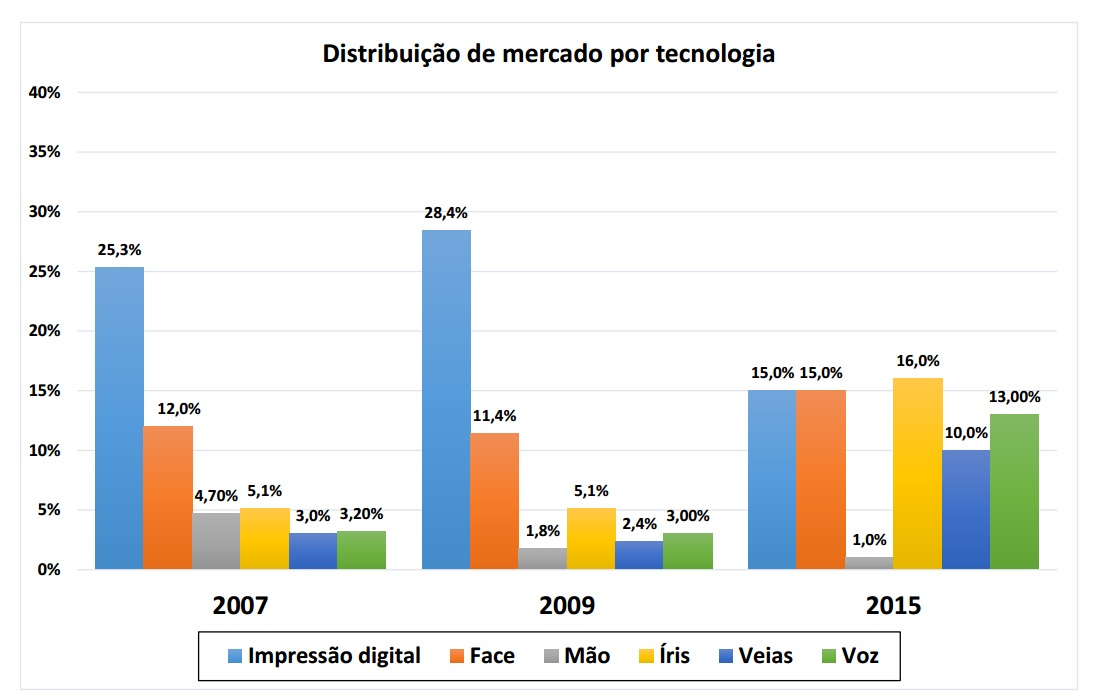
\includegraphics[scale=0.55]{figuras/cap2/mercado_bio.jpg}\\
  Fonte: Grupo de Biometria Internacional \textit{(\textit{Internacional Biometric Group$^{\copyright}$} -- IBG)} \cite{larsen2008biometric, zhang20133d, bosworth2014computer}.
  \label{mercado_bio}
  \end{center}
  \end{figure}

\nomenclature{IBG}{Grupo de Biometria Internacional (\textit{Internacional Biometric Group$^{\copyright}$})}


 Uma das desvantagens das técnicas de impressão digital é a possibilidade de fraudes. Por ser uma das tecnologias de biometria mais conhecidas \cite{bosworth2014computer}, há muitas informações sobre essa técnica disponível ao público. Apesar de não ser um processo simples, existe a possibilidade de falsificação de digital, utilizando um dedo falso produzido com látex ou outro material; ou até mesmo, em casos extremos, utilizando um dedo real amputado, pois a maioria dos leitores de impressões digitais não tem a capacidade de discriminação entre um tecido vivo e um morto. É indiscutível o fato de que a criminalidade corre contra os avanços da tecnologia, principalmente quando se trata de segurança. Portanto, é necessário conhecer as vulnerabilidades da técnica a ser utilizada para adotar medidas de correção de erros e prevenção de falhas para evitar possíveis fraudes e ataques. Outro problema enfrentado na implantação de sistemas de impressão digital para autenticação é a aceitação por parte dos usuários. Muitas pessoas não gostam de inserir o dedo no dispositivo de leitura. Outras pessoas, com receio de que o dado seja utilizado para outros fins, não aceitam a utilização do sistema por associarem a técnica à aplicações relacionadas a perícias forense, investigações criminais e a execução da lei \cite{bosworth2014computer, maltoni2009handbook}.


\subsubsection{Formação das impressões digitais}
 As impressões digitais são formadas nos sete primeiros meses de desenvolvimento do feto e não se alteram ao longo da vida do indivíduo, a não ser por motivos excepcionais, como acidentes, queimaduras ou cortes, ainda assim, tem a capacidade de se regenerar. A impressão digital ou datilograma é a reprodução do desenho digital resultante da combinação de cristas papilares e sulcos interpapilares localizados na polpa digital \cite{tavares1991papiloscopia}. As cristas papilares são os relevos epidérmicos situados na palma das mãos e na planta dos pés. Elas são separadas por depressões chamadas de sulcos interpapilares, formando assim os desenhos papilares \cite{couto2009segredos, holder2011fingerprint}, inclusive da superfície do tecido carnoso dos dedos (polpa digital)

\subsubsection{Leitura de impressão digital}
  A captura de impressão digital, bem como as técnicas e os equipamentos empregados, para fins de investigações criminais ou perícias forenses, são diferentes daqueles utilizados para fins de controle de acesso, que normalmente são mais amigáveis, mais compactos e mais baratos \cite{maltoni2009handbook}.

  Para fins de controle de acesso, as aplicações que envolvem a leitura da impressão digital podem empregar diferentes tipos de sensores que fazem a captura direta da imagem do dedo. Sem o uso de sensores específicos para a aquisição de imagens digitais dos dedos, a obtenção da imagem da digital pode ser feita por aquisição \textit{off-line}, em que ocorre a digitalização de uma imagem da impressão digital gravada em  papel.  Nesse processo, a superfície do dedo do usuário que contém o desenho digital é coberto de tinta e em seguida o dedo é pressionado contra um cartão de papel. A imagem impressa no cartão é digitalizada por um \textit{scanner}, que produz a imagem digital final que é utilizada no processo de identificação. Esse era o principal método usado por Sistemas de Identificação de Impressão Digital Automatizados (\textit{Automated Fingerprint Identification System} -- AFIS) antes do surgimento de sensores especializados. No entanto, esse processo é demorado para aplicações de controle de acesso. Assim, é necessário o uso de sensores específicos para a leitura de impressões digitais em tempo real, pois eles realizam o processo de digitalização em uma única etapa e agem mais rápido na leitura para reprodução da imagem digital. A Figura~\ref{leitor_bio} mostra o diagrama de um sistema eletrônico de leitura de impressão digital.

\nomenclature{AFIS}{Sistema de Identificação de Impressão Digital Automatizado (\textit{Automated Fingerprint Identification System})}


  Na Figura~\ref{leitor_bio}, o leitor representa o módulo interno ao aparelho, responsável por capturar a imagem da superfície do dedo. Essa imagem é convertida de analógica para um padrão digital. A imagem digital gerada na conversão A/D é enviada para um dispositivo externo, geralmente um computador, através de uma interface de comunicação responsável também pela troca de outras informações com o dispositivo. 
  
  
  Atualmente existem diversos tipos de sensores, mas quase todos são baseados em tecnologia ótica,  estado sólido ou ultrassom. Assim, a imagem adquirida por cada um desses sensores pode gerar diferentes resultados, conforme mostrado no exemplo da Figura~\ref{tipos_sensores}.


  \begin{figure}[!b]
  \begin{center}
  \caption{Diagrama de blocos de um sistema eletrônico de leitura de impressão digital.}
  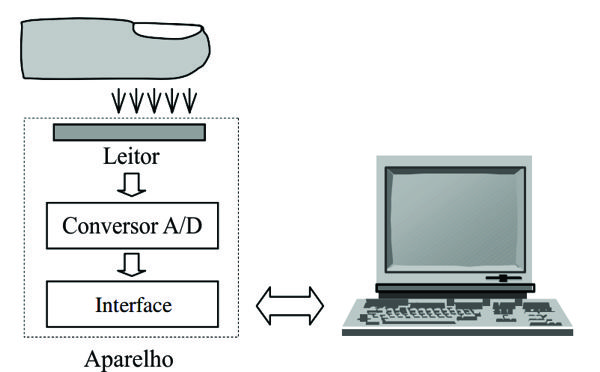
\includegraphics[scale=0.6]{figuras/cap2/leitor_bio.jpg}\\
  Fonte: Adaptado de \cite{maltoni2009handbook}.
  \label{leitor_bio}
  \end{center}
  \end{figure}


  \begin{figure}[!t]
  \begin{center}
  \caption{Imagens de impressão digital: a) sensor óptico; b) sensor capacitivo; c) sensor piezoelétrico; d) sensor térmico.}
  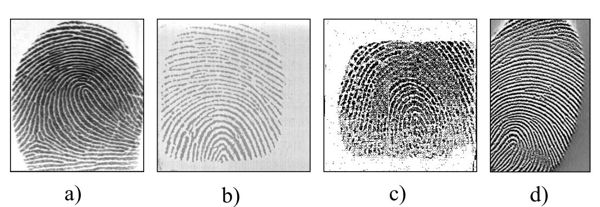
\includegraphics[scale=0.75]{figuras/cap2/tipos_sensores.jpg}\\
  Fonte: Adaptado de \cite{maltoni2009handbook}.
  \label{tipos_sensores}
  \end{center}
  \end{figure}


\subsubsection{Extração de características}
  A imagem da impressão digital é formada pela disposição de cristas (linhas escuras) e vales (linhas claras), como mostra a Figura~\ref{cristas_vales}. Através dessa disposição, é possível gerar um modelo de características para a identificação de usuários. Essas características são extraídas a partir do reconhecimento de terminações ou bifurcações de saliências, chamadas de \textit{minúcias}, e de outros elementos, como \textit{delta} e \textit{núcleo}, ilustrados na Figura~\ref{nucleo}, que são denominados \textit{regiões singulares}. O \textit{delta} é o ângulo ou triângulo formado pelas cristas papilares; e o \textit{núcleo} é um ponto central localizado na polpa da digital e pode ser também definido como um \textit{laço} [veja as Figuras~\ref{regioes_singulares}(a) e ~\ref{regioes_singulares}(b)] ou \textit{espiral} [mostrado na Figura~\ref{regioes_singulares}(c)]. Quando a digital não contém um laço ou espiral é difícil definir um núcleo. Desta forma, em alguns casos a região pode ser classificada como \textit{arco} (Figura~\ref{regioes_singulares} - d).  Além de bifurcações e terminações existem outros tipo de minúcias, na Tabela~\ref{tipos_minucias} são listados os tipos mais comuns de minúcias.



  \begin{figure}[!ht]
  \begin{center}
  \caption{Cristas e vales em uma imagem de impressão digital.}
  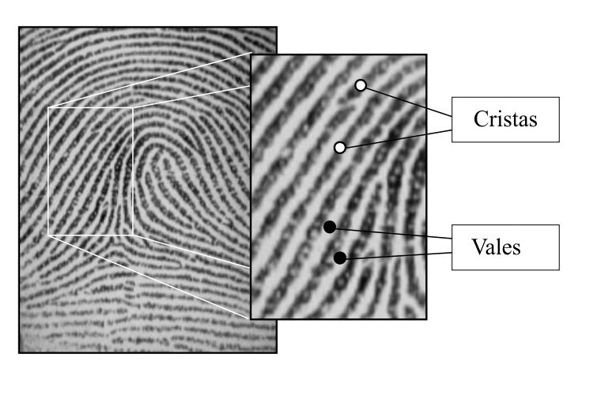
\includegraphics[scale=0.6]{figuras/cap2/cristas_vales.jpg}\\
  Fonte: Adaptado de \cite{maltoni2009handbook}.
  \label{cristas_vales}
  \end{center}
  \end{figure}
  
 
  \begin{figure}[!ht]
  \begin{center}
  \caption{Núcleo e delta em um imagem de impressão digital.}
  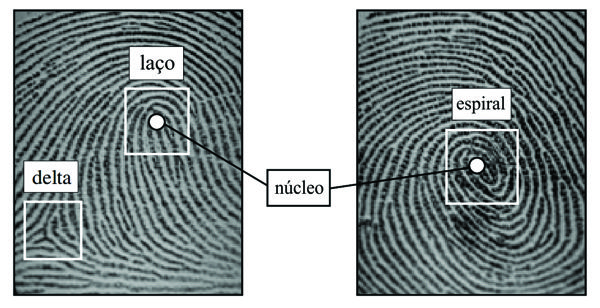
\includegraphics[scale=0.7]{figuras/cap2/nucleo.jpg}\\
  Fonte: Adaptado de \cite{maltoni2009handbook}.
  \label{nucleo}
  \end{center}
  \end{figure}
 
  \begin{figure}[!ht]
  \begin{center}
  \caption{Impressões digitais caracterizada por por \textit{laço} à esquerda e à direita, \textit{espiral} e \textit{arco}.}
  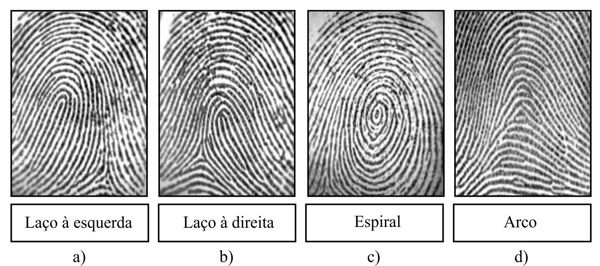
\includegraphics[scale=0.8]{figuras/cap2/regioes_singulares.jpg}\\
  Fonte: Adaptado de \cite{maltoni2009handbook}.
  \label{regioes_singulares}
  \end{center}
  \end{figure}
  
  
  \begin{table}[]
  \centering
  \caption{Os tipos mais comuns de minúcias.}
  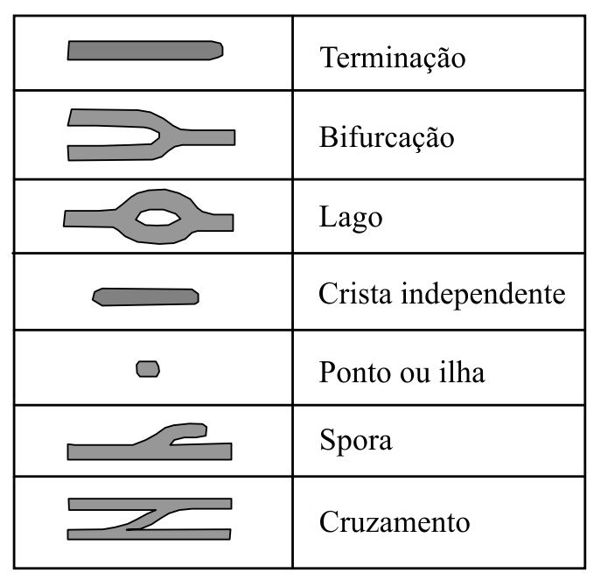
\includegraphics[scale=0.54]{figuras/cap2/tipos_minucias.jpg}\\
  Fonte: Adaptado de \cite{maltoni2009handbook}.
  \label{tipos_minucias}
  \end{table}
  
  
  A partir do uso das características citadas, existem várias técnicas e algoritmos desenvolvidos para o processamento e reconhecimento de impressões digitais na literatura biométrica \cite{bhanu2012computational, sarfraz2005computer, ratha2007automatic, alonso2007comparative, tico2001fingerprint, calabaide2006biometria}. Isso inclui, necessariamente, o uso de diferentes técnicas de processamento de imagens para extração de características e geração de modelo para comparação de usuários nos processos de verificação e autenticação. As abordagens de reconhecimento de digitais são basicamente divididas em três categorias \cite{maltoni2009handbook}: 
  
  \begin{itemize}
  \item Baseado em correlação
      
  Duas imagens de impressões digitais, no nível de tons de cinza, são sobrepostas e a correlação entre os \textit{pixels} correspondentes é computada mediante diferentes alinhamentos, deslocamentos e rotações.

  \item Baseado em minúcias
  
  \textit{Minúcias} são extraídas de duas impressões digitais e armazenadas como conjuntos de pontos no plano bidimensional (\textit{template}). O reconhecimento baseado em \textit{minúcias} consiste essencialmente de encontrar o alinhamento entre o modelo armazenado e o modelo a ser comparado. Isso resulta em um número máximo de \textit{minúcias} semelhantes.


  \item Baseado em cristas
 
  A extração de \textit{minúcias} é difícil em imagens de impressão digital de baixa qualidade, mas existem outras características do padrão de crista da digital, como orientação local, frequência, forma e informações de textura, podem ser extraídas com mais segurança que as \textit{minúcias}, mesmo que a distinção dessas características de crista sejam inferiores.

  \end{itemize}
  
  
  Portanto, qualquer técnica de reconhecimento de impressão digital gera o seu modelo de características baseada em uma dessas abordagens para a comparação de digitais.
  


\subsubsection{Sistemas biométricos}

  Dependendo do contexto da aplicação, todo sistema biométrico pode ser classificado de forma geral, como um \textit{sistema de identificação} ou \textit{sistema de  autenticação}, e ambos dispõe de três modos essenciais de operação: 

\begin{itemize}
     

\item Registro

  No registro é obtido o dado biométrico. Nesse processo é criado um modelo (\textit{template}), a partir da extração da característica biométrica do usuário. Cada usuário recebe um número de identificação pessoal(\textit {Personal Identification Number} -- PIN), que é vinculado ao seu modelo biométrico 
  armazenado no banco de dados, para posterior comparação nas operações de verificação (autenticação) e identificação. Na Figura~\ref{registro}, tem-se o diagrama da operação de registro. 

\nomenclature{PIN}{Número de identificação pessoal  (\textit{Personal Identification Number})}

 \begin{figure}[!ht]
  \begin{center}
  \caption{Sistema biométrico: registro.}
  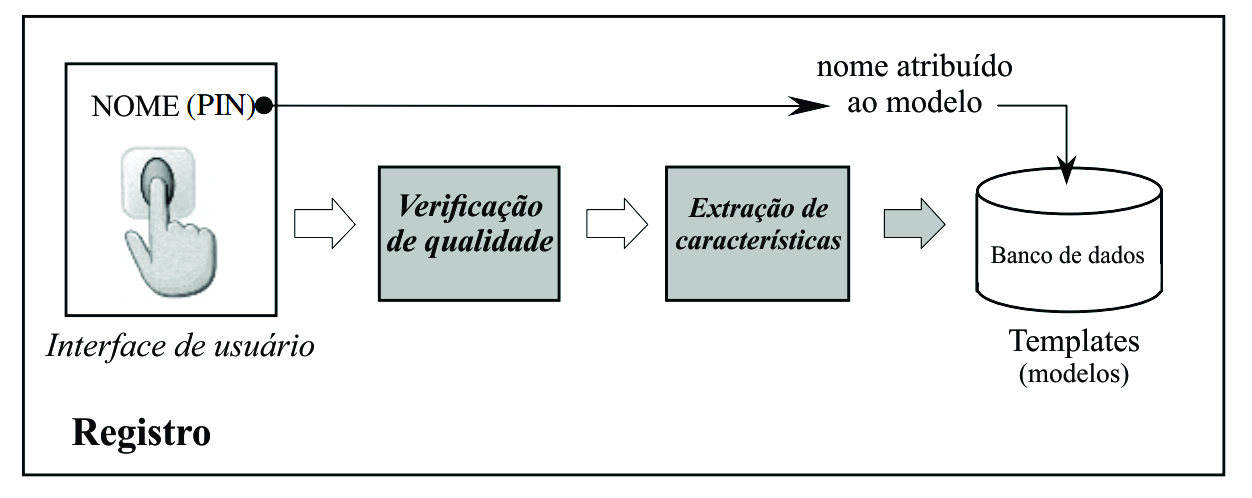
\includegraphics[scale=0.45]{figuras/cap2/registro.jpg}\\
  Fonte: Adaptado de \cite{maltoni2009handbook}.
  \label{registro}
  \end{center}
  \end{figure}
 


\item Verificação ou autenticação 

  No processo de verificação, também conhecido como autenticação, a característica biométrica do usuário que tenta autenticar-se é coletada e comparada a um único modelo. No entanto, não trata-se de qualquer modelo, pois o \textit{template} gerado na leitura é comparado especificamente com o modelo, no banco de dados, que possui o PIN informado informado pelo usuário. A Figura~\ref{verificacao} ilustra o diagrama dessa operação. 

 \begin{figure}[!ht]
  \begin{center}
  \caption{Sistema biométrico: verificação.}
  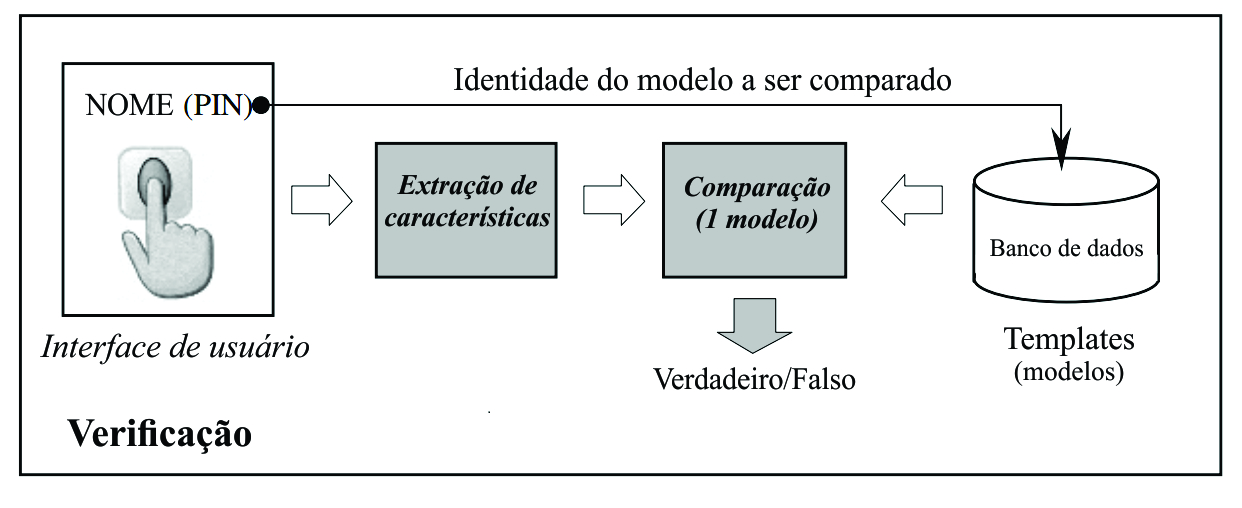
\includegraphics[scale=0.45]{figuras/cap2/verificacao.jpg}\\
  Fonte: Adaptado de \cite{maltoni2009handbook}.
  \label{verificacao}
  \end{center}
  \end{figure}

\item Identificação

  A identificação é um processo que compara a característica biométrica do usuário a ser identificado, com a característica biométricas de todos os usuários cadastrados no banco de dados. Por isso, é um processo custoso em termos de processamento. Essa operação requer que o dado biométrico de um determinado usuário seja lido e comparado a todos os modelos armazenados no banco de dados, a fim de obter como resultado um conjunto de possíveis usuários, uma lista com as identificações que apresentarem maior similaridade em relação as características do usuário em questão. O diagrama desse processo é mostrado na Figura~\ref{identificacao}

 \begin{figure}[!ht]
  \begin{center}
  \caption{Sistema biométrico: identificação.}
  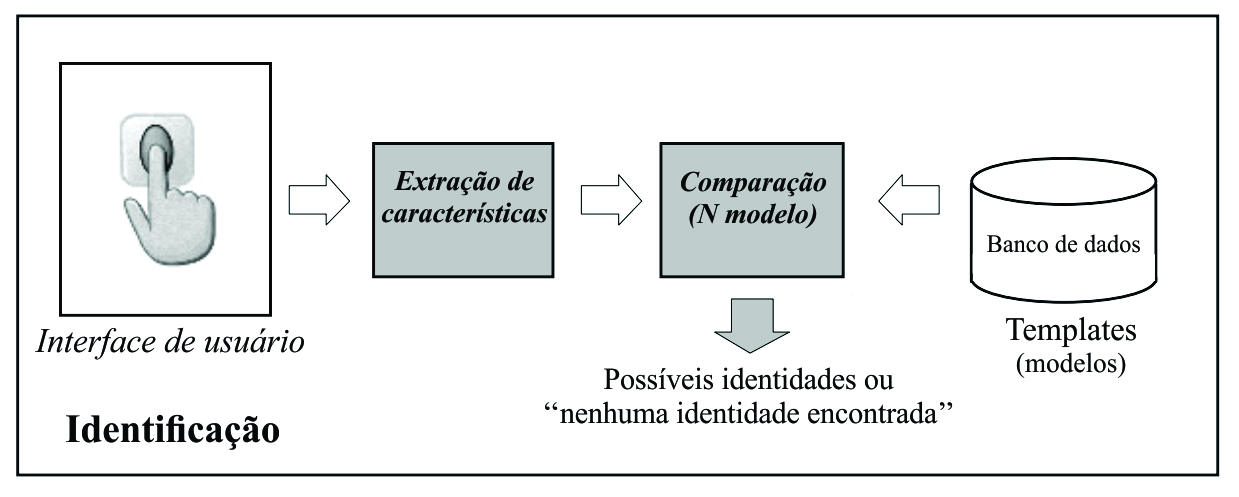
\includegraphics[scale=0.45]{figuras/cap2/identificacao.jpg}\\
  Fonte: Adaptado de \cite{maltoni2009handbook}.
  \label{identificacao}
  \end{center}
  \end{figure}

\end{itemize}



\section{Arduino}

   O Arduino é uma plataforma de \textit{hardware} \textit{open source}, ideal para a criação de dispositivos de entrada e saída que permitam interação com o ambiente \cite{arduino}, possui sua própria interface de programação e utiliza uma linguagem de alto nível, tornando fácil a sua utilização para desenvolvedores. Tal plataforma utiliza uma camada simples de \textit{software} implementada no \textit{hardware}, o \textit{bootloader}, e uma interface de fácil usabilidade para programação. O processamento do \textit{hardware} é realizado por microcontroladores e cada versão da placa apresenta um microcontrolador diferente. Normalmente é necessário utilizar um dispositivo específico para programar um microcontrolador. No entanto, essa programação é possível através da instalação de um sistema de instruções operacionais (\textit{firmware} ou \textit{bootloader}) no microcontrolador, que permite a instalação (programação) de novas instruções através de um programador externo (interface de computador) \cite{arduinocc_bootloader}. A interface de programação da placa utiliza a linguagem \textit{Processing}, a qual é baseada na linguagem C/C++ e também é \textit{open source}. Através do bootloader dispensa-se o uso de dispositivos programadores para o chip -- no caso a família AVR do fabricante ATMEL -- facilitando ainda mais o seu uso uma vez que não exige compiladores ou \textit{hardware} adicional. Neste ambiente de desenvolvimento, são disponibilizadas bibliotecas que permitem o interfaceamento com outros \textit{hardware}, permitindo o completo desenvolvimento de aplicações simples ou complexas.

   A plataforma original do Arduino, mesmo tendo restrições de memória, possuía grandes possibilidades com seis entradas analógicas, 1 UART, I2C, SPI e 6 PWMs. Hoje, na mesma linha, tem-se modelos que permitem até 16 entradas analógicas, 14 PWMs, 4 UARTs, e com memória comparável a plataformas complexas como a família ARM. A placa Arduino se conecta ao computador através de uma porta USB (Universal Serial Bus)  e disponibiliza saídas de tensão DC de $3.3$ V, $5$ V e $9$ V (quando alimentada por fonte externa) e que podem ser usadas em circuito auxiliares de baixo consumo, aumentando significativamente a sua versatilidade.
   
   \nomenclature{USB}{\textit{(Universal Serial Bus)}}
   
   
\subsection{Serial}
  
   A interface Serial é usada para comunicação entre a placa Arduino e um computador ou outros dispositivos. Todas as versões do Arduino tem pelo menos uma porta serial, também conhecida como UART, USART ou apenas Serial. Das três vias que compõem um barramento serial, apenas duas são de dados, como ilustra a Figura~\ref{serial}, sendo uma para enviar dados (TX) e outra para receber (RX). No Arduino essa comunicação funciona através dos pinos 0 (RX) e 1 (TX) da mesma forma que o computador opera via USB. Portanto, se essa função for utilizada, os pinos 0 e 1 não poderão ser utilizados como entrada/saída digital \cite{russell, arduinocc_serial}. 
  
  \begin{figure}[ht]
  \begin{center}
  \caption{Comunicação serial - vias de dados.}
  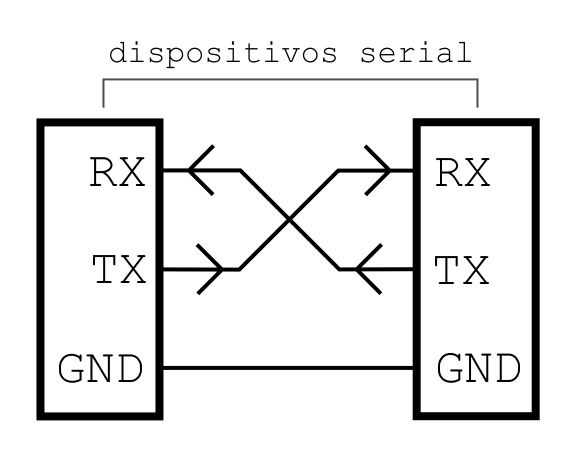
\includegraphics[scale=0.5]{figuras/cap2/serial.jpg}\\
  Fonte: Elaborada pelo autor.
  \label{serial}
  \end{center}
  \end{figure}


  A taxa de transmissão de dados é ajustável e definida em bits por segundo (baud) na função \textit{begin()}, onde podem ser empregadas as taxas recomendadas pelo fabricante (300, 600, 1200 etc) ou uma taxa específica para comunicação pelos pinos 0 e 1 com componentes que requeiram uma taxa de bits por segundo particular. Além disso, esses pinos podem ser usados para comunicação com dispositivos externos TTL serial conectando o pino RX do Arduino ao pino TX do dispositivo e o pino TX no RX do dispositivo.  

  Vale ressaltar que os pinos de comunicação serial do Arduino operam sob o padrão TTL e não podem ser conectados diretamente a uma porta serial RS-232, pois este padrão opera em nível de tensão $\pm 12$ V e pode danificar a placa. Desta forma, o \textit{hardware} serial envia e recebe dados na forma de pulsos elétricos que representam sequências de bits. Os zeros e uns que carregam a informação que compõe um byte podem ser representados de várias formas. No Arduino 0 volt representa um bit de valor \textbf{0} e 5 volts (ou 3.3 volts) representa um bit de valor \textbf{1}.

  Além dos padrões TTL e RS-232, existem outros protocolos de comunicação serial utilizados em aplicações de \textit{hardware}. O I$^{2}$C, por exemplo, é um padrão serial utilizado em componentes compatíveis com o Arduino, como módulos RTC (\textit{Real Time Clock}), módulo para \textit{display} LCD e chip expansor de portas. A seguir, o I$^{2}$C, juntamente com o TTL e o RS-232 são descritos sucintamente.

  \nomenclature{RTC}{Relógio de Tempo Real (\textit{Real Time Clock})}  

  \begin{itemize}
  \item{TTL} 
  
  O padrão que utiliza 0 volt para representar o bit 0 e 5 volts para o bit 1 é muito comum e conhecido como nível TTL, pois assim é como os sinais eram representados em uma das primeiras implementações de lógica digital, chamado de Lógica Transistor-Transistor (\textit{Transistor-Transistor Logic} -- TTL).
  Algumas placas têm um chip que converte a porta serial para o padrão USB, já aquelas que não dispõe de suporte para esse padrão, requerem um adaptador, que converte TTL para USB, para servir a conexão com um computador \cite{arduinocookbook}.
 
  
  \nomenclature{TTL}{Lógica Transistor-Transistor (\textit{Transistor-Transistor Logic})}
  
  \item{RS-232}
  
  O RS-232 é um antigo protocolo de comunicação que usa um nível de voltagem (+/- 12V) incompatível com os pinos digitais do Arduino -- por isso a necessidade do uso de um conversor RS-323/TTL  -- e normalmente tem nove pinos. A vantagem desse padrão sobre o TTL está na distância limite que ele alcança que é de 80 a 130 ft (pés) ou 24,384 a 39,624 metros, dependendo da taxa de bits e do tipo de cabo, enquanto que o USB chega a 16 ft ou 4,8768 m.


 \item{I$^{2}$C}
 
   Em projetos com Arduino, por exemplo, o Circuito Inter-integrado (\textit{Inter-Integrated Circuit} -- I$^{2}$C) é utilizado para tornar o circuito compacto, reduzindo a quantidade de fios e trilhas necessários para conectar os periféricos, como sensores, displays, teclados, leds, buzzers, etc, ou seja, todos aqueles dispositivos que utilizam pinos digitais para interagir com o microcontrolador. Caso esses dispositivos não sejam compatíveis com o I$^2$C, utilizam-se conversores ou chips que possibilitem a integração da tecnologia.
 
 \nomenclature{I$^{2}$C}{Circuito Inter-integrado (\textit{Inter-Integrated Circuit})}
 
   O I$^{2}$C é um barramento serial bidirecional desenvolvido pela Philips Semiconductors (agora NXP Semiconductors), usado para conectar periféricos de baixa velocidade a um computador, sistema embarcado ou celular. Esse barramento requer apenas duas vias para estabelecer a comunicação: uma via de dados serial (SDA - Seial Data) e uma via de clock serial (SCL - Serial Clock) \cite{i2c}. A Figura~\ref{i2c} mostra um exemplo de aplicação desse padrão.
 
 \begin{figure}[ht]
  \begin{center}
  \caption{Exemplo de aplicação I$^{2}$C.}
  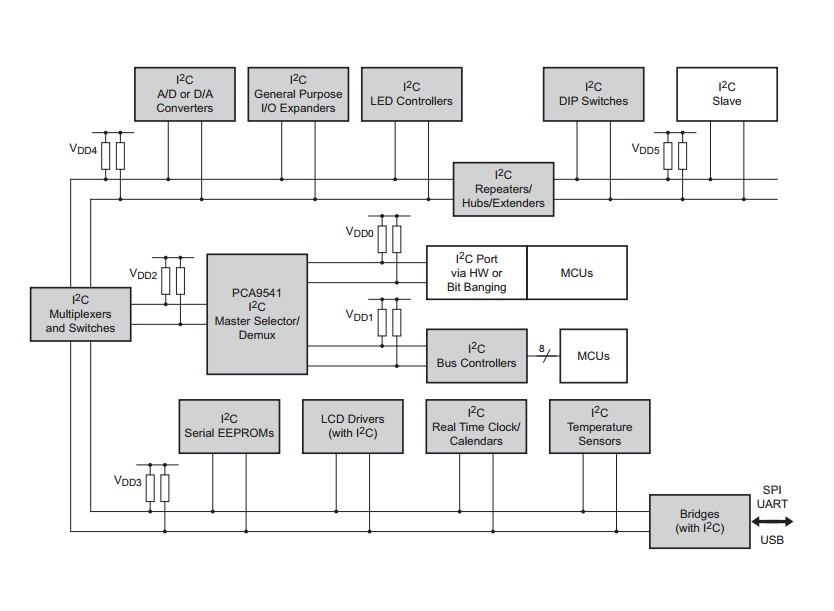
\includegraphics[scale=0.7]{figuras/cap2/i2c_app.jpg}\\
  Fonte: Adaptado de I$^{2}$C-bus specification and user manual\cite{i2c}.
  \label{i2c}
  \end{center}
  \end{figure}
  %\newpage
  
   A principal vantagem do uso desta tecnologia é que, por se tratar de um barramento multimestre, com apenas duas vias (dados e clock) é possível conectar vários dispositivos no mesmo barramento, cada um identificado por um endereço específico. O endereço atribuído a cada elemento no circuito normalmente é composto por 7 bits e isso dá um limite teórico de até 127 dispositivos em uma conexão \cite{arduinocc_i2c}. Além disso, eles podem ser configurados para receber ou transmitir dados e classificados como \textit{master} (mestre) ou \textit{slave} (escravo), onde o \textit{master} é o responsável por iniciar a comunicação e enviar informações a determinado \textit{slave} e este é encarregado somente por responder ao \textit{master}.
 \end{itemize}
 
 
 \section{Node.js}
 
   Apresentado em 2009 na JSConf Europa, por Ryan Dahl, o NodeJS é uma plataforma utilizada para a construção fácil e rápida de aplicações de rede escaláveis, em relação a outros programas de servidor como Apache ou o Tomcat.
   No lado do servidor, o Node funciona através da execução do V8 JavaScript. O V8 é um mecanismo subjacente da \textit{engine JavaScript open source}, um interpretador de alta performance escrito em C++, criado pela empresa de tecnologia Google que utiliza-o em seu navegador Chrome (no lado do cliente). No lado do cliente, a engine JavaScript interpreta e executa o código. Desta forma, é possível baixar o mecanismo e integrá-lo em qualquer aplicativo, pois ele não é restrito à execução em um navegador; o Node simplesmente usa esse mecanismo e o redireciona para uso no servidor.
 
   O principal destaque do Node é oferecer uma maneira mais fácil de criar aplicações de rede escalonáveis, pois o problema com os programas de servidor atuais, em linguagens como Java™ e PHP, é que a cada conexão feita no servidor é criada uma nova \textit{thread} que aloca 2 MB de memória. Nesse cenário, em um sistema com 8 GB de memória RAM, por exemplo, o número máximo teórico de conexões simultâneas fica limitado em torno de 4.000 usuários. Com o aumento do número de usuários seria necessário adicionar mais servidores, o que geraria mais custos operacionais e problemas técnicos. Assim, o Node busca solucionar esse problema criando um processo a cada conexão, o qual não requer a alocação de um novo espaço de memória, possibilitando o suporte a dezenas de milhares de conexões simultâneas. Ele aguarda eventos específicos, e quando um evento ocorre ele é respondido imediatamente. Enquanto um evento é processado, o Node não recusa qualquer outro pedido, ou seja, a resposta a outros eventos não depende que o atual seja concluído, os eventos são processados de forma que o primeiro que entra é o primeiro que sai em um \textit{event loop} \cite{nodejs, nodejs3}, como mostra a Figura~\ref{nodejs:eventloop}.  Assim, o modelo de programação do Node é orientado a eventos e apresenta uma sintaxe familiar, até para programadores iniciantes, que torna a implementação do \textit{software} mais fácil de codificar.
 
  \begin{figure}[!t]
  \begin{center}
  \caption{\textit{Event loop} do Node.js.}
  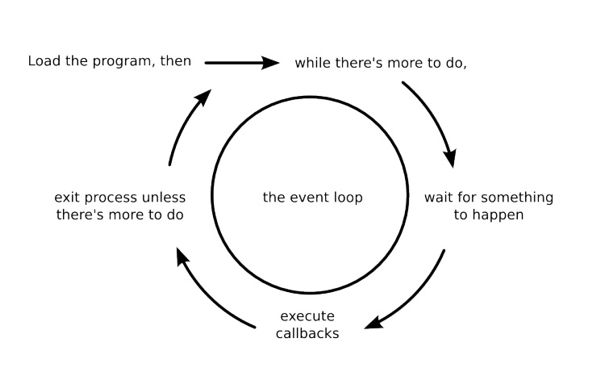
\includegraphics[scale=0.7]{figuras/cap2/nodejs_loop.jpg}\\
  Fonte: Adaptado de \cite{nodejs2}.
  \label{nodejs:eventloop}
  \end{center}
  \end{figure}
  %\newpage
 
   O Node é largamente empregado na construção de aplicações web. No entanto, a sua abrangência vai além de aplicações web, através do Node.js é possível escrever ferramentas de linha de comando, desenvolver aplicativos nativos para diferentes sistemas operacionais e construir aplicações \textit{desktop}. O Electron \cite{electron.atom}, por exemplo, é uma plataforma que permite a construção de apps desktop utilizando Node.js. Portanto, O Node é excelente para uma ampla gama de aplicações \cite{nodejs2}.

 
\section{SQL}
 
  SQL é uma linguagem de consulta estruturada de propósito especial usada para definir, acessar e manipular dados. É uma linguagem padrão universal para manipular banco de dados relacionais, além de ser não procedural, isto é, não é baseiada em sequências de prodedimentos/rotinas. 
 
 
 \section{MySQL}
 
  O MySQL é um sistema gerenciador de banco de dados relacional (SGBDR) gratuito e \textit{open source} que utiliza a linguagem SQL, sendo um dos mais populares do mundo. O MySQL é caracterizado pela sua rapidez, flexibilidade e segurança, além de ser relativamente simples~\cite{dubois2013}. 


\section{Placa de Circuito Impresso (PCB)}

  Um circuito impresso ou placa de circuito impresso (\textit{printed circuit board} -- PCB) consiste de um painel de material isolante, como Fenolite ou Fibra de Vidro, com uma fina camada de cobre condutor depositada sobre uma ou duas de suas faces através de um processo eletroquímico. As PCB's comuns, usadas em processos de confecção manual, podem ser de face única ou dupla, porém, as placas fabricadas em processos industriais, como placas de computador, celular ou outras produzidas em larga escala, são compostas de várias camadas de placas moldadas e integradas por meio de furos condutores. A camada de cobre sobre uma face constitui as trilhas condutoras que representam o circuito onde serão soldados e interligados os componentes eletrônicos. O processo de confecção de PCB's pode ser realizado empregando diversas técnicas existentes, sendo elas manuais ou industriais. O processo manual envolve algumas etapas fundamentais que são descritas a seguir \cite{pcb, pcb2}.

\nomenclature{PCB}{Placa de circuito impresso (\textit{Printed Circuit Board})}

\begin{enumerate}

\item \textbf{Projeto do circuito}

  Utilizando uma PCB virgem, um painel com face inteiramente coberta por camada de cobre, é feita a gravação de ``trilhas'' de cobre responsáveis por conectar os componentes de um circuito e substituir fios condutores. Em um processo manual, primeiramente, é necessário um \textit{software} de projeto de circuitos para desenhar as trilhas, como mostra a Figura~\ref{designcircuit}.


  \begin{figure}[ht]
  \begin{center}
  \caption{Design de circuito projetado no \textit{software} EAGLE 7.5.0 Light.}
  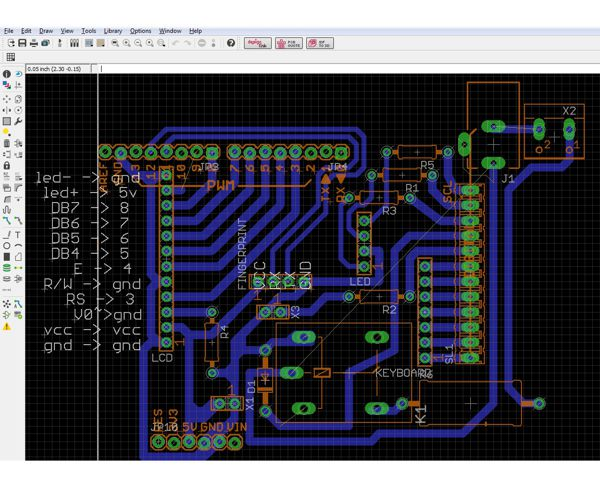
\includegraphics[scale=0.8]{figuras/cap2/designcircuit.jpg}\\
  Fonte: Elaborada pelo autor
  \label{designcircuit}
  \end{center}
  \end{figure}

  
  

\item \textbf{Impressão do design}
 
  A partir do layout do circuito mostrada na Figura~\ref{designcircuit}, é feita a impressão (Figura~\ref{impressdesigncircuit}) do design que representa o circuito, preferencialmente, em papel fotográfico para facilitar o processo térmico de transferência, e necessariamente em impressora a laser. 

  \begin{figure}[ht]
  \begin{center}
  \caption{Impressão do design do circuito para transferência.}
  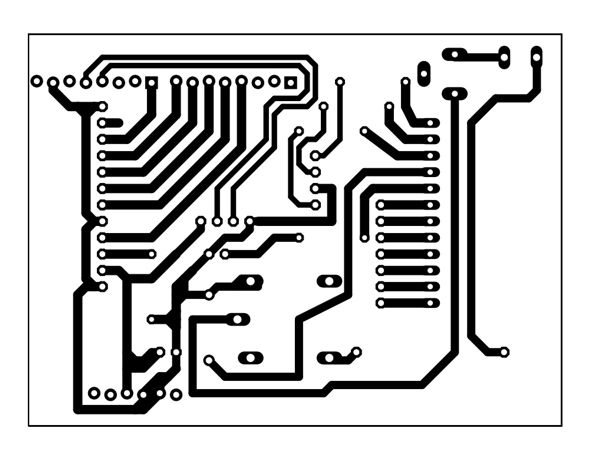
\includegraphics[scale=0.5]{figuras/cap2/impresscircuit.jpg}\\
  Fonte: Elaborada pelo autor
  \label{impressdesigncircuit}
  \end{center}
  \end{figure}
  


\item \textbf{Transferência} 

  De posse do design impresso, é feita a transferência da impressão para a placa virgem, normalmente, utilizando uma impressora de transferência térmica ou um ferro de passar roupas. Nesse processo, o toner presente no papel é termicamente transferido para a superfície de cobre da placa, assim, as regiões que representam o circuito cobrem a superfície de cobre da placa virgem, como mostra a Figura~\ref{designcircuit2}.

  \begin{figure}[!ht]
  \begin{center}
  \caption{Transferência do design impresso do circuito.}
  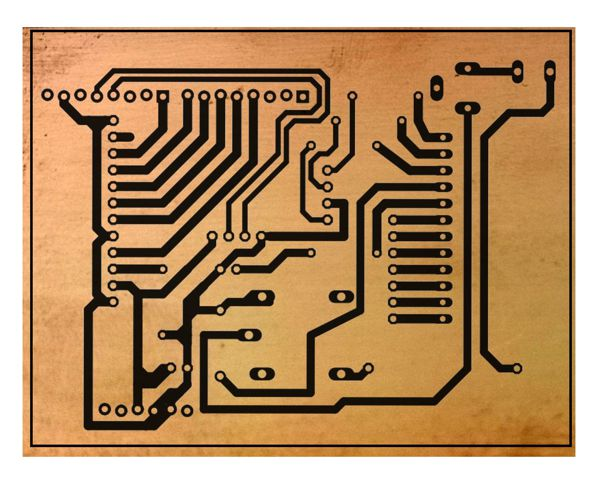
\includegraphics[scale=0.5]{figuras/cap2/impresscircuit2.jpg}\\
  Fonte: Elaborada pelo autor
  \label{designcircuit2}
  \end{center}
  \end{figure}





\item \textbf{Corrosão} 

  Nesta etapa deve ser feita a corrosão das regiões de cobre expostas, o que consiste em remover aquelas partes não cobertas por toner ou qualquer outro material que proteja e isole o cobre. O processo químico de corrosão ocorre utilizando-se soluções ácidas a partir de compostos químicos, como o Percloreto de Ferro ou outros, que em contato direto com o cobre reagem, retirando-o do painel de material isolante, deixando intactas apenas as regiões protegidas, ou seja, as trilhas do circuito, assim obtemos o resultado da Figura~\ref{designcircuit3}. O Cloreto Férrico ou Percloreto de Ferro, é um sal que em solução aquosa desenvolve ação corrosiva, e desta propriedade obtém-se marcações ou gravuras em metais \cite{gravuraemmetal}.

  \begin{figure}[!ht]
  \begin{center}
  \caption{Corrosão da superfície de cobre exposta.}
  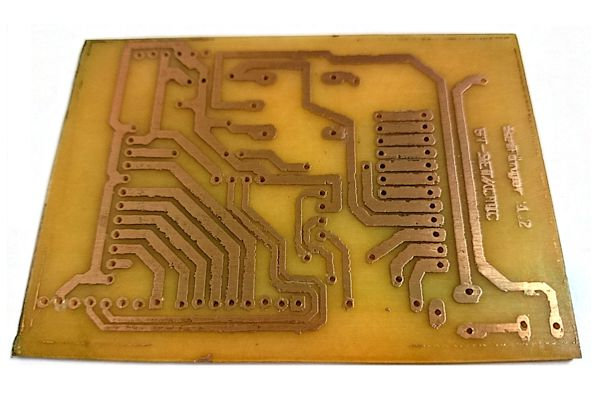
\includegraphics[scale=0.6]{figuras/cap2/impresscircuit3.jpg}\\
  Fonte: Elaborada pelo autor
  \label{designcircuit3}
  \end{center}
  \end{figure}



\item \textbf{Perfuração} 

  Após a gravação do layout do circuito na placa virgem é feita a sua furação nas respectivas ilhas de cobre, pontos onde os componentes serão conectados, utilizando um perfurador manual ou uma furadeira.

\item \textbf{Montagem e soldagem}

  Para finalizar, é feita a montagem e soldagem dos componentes em seus respectivos espaços na placa. Após está etapa, o circuito está pronto para testes e uso.


\end{enumerate}
\chapter{Soluções eletrônicas de controle de acesso físico \label{cap:estadodaarte}}


\section{Introdução}

O controle de acesso é uma área da Segurança bastante explorada que oferece uma gama de soluções eletrônicas, principalmente utilizando biometria. Além da variedade e quantidade de soluções encontradas no mercado, existem também muitas propostas de soluções de controle de acesso de cunho cientifico, voltadas para atender a comunidade acadêmica ou para suprir as necessidades da sociedade em geral, oferecendo soluções que ainda não foram produzidas pela indústria. Este capítulo abordada algumas propostas acadêmicas de controle de acesso utilizando cartões eletrônicos de identificação, impressão digital e multibiometria; e apresenta os principais produtos eletrônicos de controle de acesso físico comercializados no mercado de segurança. 


\section{Soluções acadêmicas \label{solucoes_academicas}}
A seguir são apresentadas as soluções eletrônicas de controle de acesso, de caráter cientifico, divididas por tecnologia.



\subsection{Impressão digital}

 Sanchez~\cite{sanchez2011registro} propõe a automatização do processo de registro de frequência de estudantes nas Instituições de Ensino utilizando biometria da impressão digital. O foco da aplicação proposta por ele concentra-se no desenvolvimento de um algoritmo de processamento de digitais e na sua otimização para reduzir o custo de busca de registros. 
 Conforme o trabalho, a identificação dos discentes deve ser realizada em sala de aula, de modo que, o aluno precisa apenas inserir seu dedo em um leitor biométrico. O leitor captura a imagem da impressão digital para que o sistema identifique automaticamente a identidade do usuário e registre a sua presença em sala de aula, não havendo a necessidade de qualquer outro tipo de interação. A solução proposta foi desenvolvida utilizando o Kit de Desenvolvimento de Software (\textit{Software Development Kit} -- SDK) da empresa de tecnologia biométrica \textbf{Griaule Biometrics}. A partir do SDK o autor utilizou uma Interface de Programação de Aplicações (\textit{Application Programming Interface} -- API) que disponibiliza mecanismos para a captura da imagem de impressões digitais através de um sensor pré-configurado. 
 
 \nomenclature{SDK}{Kit de Desenvolvimento de Software (\textit{Software Development Kit})}
 
 
 Canedo \cite{canedo2003terminal} tem como objetivo a criação de um terminal biométrico de baixo custo para atender as demandas do mercado de controle de acesso e ponto por soluções que forneçam maior segurança e sejam capazes de serem integradas com sistemas já existentes. Este terminal biométrico possui um leitor de impressões digitais capacitivo, um \textit{display} de cristal líquido alfanumérico, um teclado e interfaces para atuadores e sensores. Sua principal tarefa  é enviar as digitais capturadas para um programa servidor utilizando o protocolo TCP/IP sobre uma rede Ethernet 10BaseT. O servidor recebe as imagens e submete a um \textit{software} que retorna o resultado da busca, sendo necessário um banco de dados para gerenciar usuários e impressões digitais. Além disso, O programa servidor pode gerenciar centenas de terminais biométricos. 
 O \textit{software} é baseado em SDK Griaule AFIS, um conjunto completo e abrangente de componentes para segurança pública e identificação em ambiente Internet e Web, que atende aos padrões WSQ (\textit{Wavelet Scalar Quantization}) do FBI e diversos padrões do Instituto Nacional Americano de Padrões (\textit{American National Standards Institute} -- ANSI) e do  Instituto Nacional de Padrões e Tecnologia (\textit{National Institute of Standards and Technology} -- NIST). O WSQ é o padrão de compressão de imagens formulado e utilizado pelo FBI para a digitalização de imagens de impressões digitais em escala de cinza \cite{ de2007analise}. Esse padrão adota uma quantização para a decomposição da imagem em 64 sub-bandas usando a transformada discreta de \textit{wavelet} (\textit{Discrete Wavelet Transform} -- DWT), em que as imagens são produzidas com qualidade de arquivamento e com taxas de compressão em torno de 20:1 \cite{brislawn1996fbi}.
 
 
 \nomenclature{WSQ}{\textit{Wavelet Scalar Quantization}}
 \nomenclature{ANSI}{Instituto Nacional Americano de Padrões (\textit{American National Standards Institute})}
 \nomenclature{NIST}{Instituto Nacional de Padrões e Tecnologia (\textit{National Institute of Standards and Technology})}
 \nomenclature{DWT}{Transformada Discreta de Wavelet (\textit{Discrete Wavelet Transform})}
 


Braga \textit{et al} \cite{stephanie2014control} apresentam um projeto de extensão para estudo de caso de um sistema de controle de acesso por biometria que consiste em um sistema embarcado capaz de controlar o acesso a um determinado ambiente, habilitando a entrada de pessoas somente por meio da impressão digital. O controle de acesso físico é feito por meio de uma tranca elétrica, que é acionada pelo sistema embarcado para a abertura de uma porta. A interface física com o usuário dispõe de um botão e três LEDs de sinalização. O botão deve ser pressionado sempre que o usuário desejar acesso ao ambiente controlado. Após o acionamento do botão o sensor biométrico é ativado e o LED amarelo é ligado, permanecendo assim até que o usuário insira o dedo no sensor. Se a digital do usuário for reconhecida o LED verde será ligado, caso contrário o LED vermelho será ativado. Na elaboração do sistema embarcado, foi confeccionada uma placa de circuito impresso que contém o circuito básico para receber o microcontrolador Atmega 328, os três LED's de sinalização, um botão, um circuito com relé, um circuito RS232 e o circuito de alimentação da placa.
 


 Duarte Neto \textit{et al} \cite{neto2014sistemas} apresentam um estudo de caso, no qual propõe um sistema automático de impressões digitais, utilizando um leitor biométrico ZFM-20 Adafruit, plataforma Arduino e uma aplicação Java. O programa foi implementado em Java e tem como objetivo controlar a execução das tarefas programadas no Arduino. O \textit{software} possui dois modos de operação: cadastro e identificação. O modo cadastro realiza um pré-cadastro na aplicação Java com os dados do indivíduo; no modo identificação o Arduino aguarda a leitura da impressão digital no leitor, para posterior comparação com as digitais armazenadas em sua \textit{flash}. Em ambos os modos, há notificações em um LCD ligado ao Arduino e na aplicação Java com mensagens via interface. A comunicação entre a interface Java (computador) e o sistema embarcado (\textit{hardware}), responsável pela leitura da digital, é feita via porta serial. Esse trabalho concentra-se basicamente no desenvolvimento de um \textit{software} para controlar a execução de operações do Arduino, via computador, tendo como estudo de caso a aplicação de leitura biométrica para autenticação de usuários \cite{neto2014sistemas}.


 
  Cruz \cite{cruz2013biometria} propõe o desenvolvimento de uma solução de controle de acesso para segurança residencial, através da implementação de um \textit{software} para autenticação de digitais utilizando um sensor Finger Key HamsterDx em conjunto com um SDK, de código aberto, disponibilizado gratuitamente pelo fabricante (Nitgen). Nesse trabalho foi desenvolvido uma interface de comunicação entre \textit{hardware} e \textit{software} através da manipulação do acesso a porta paralela via programação, para fazer o controle da leitura de impressões digitais no sensor. Através dessa comunicação é feita a leitura da digital e posteriormente a sua autenticação. O sistema conta ainda com um banco de dados para cadastro de usuários e suas respectivas digitais. Todo esse sistema foi desenvolvido para controlar o acesso físico de pessoas em ambientes residenciais e é conectado a uma fechadura eletrônica. A fechadura possui um controle remoto que foi conectado ao sistema pela porta paralela. Portanto, o sistema, faz a leitura e o reconhecimento da impressão digital e manipula o dispositivo (controle remoto) para controlar a fechadura eletrônica instalada na porta.


 
 Utilizando biometria e tecnologia móvel, Mocellin \textit{et al} \cite{mocellin2012trava} desenvolveram um sistema para controle de acesso utilizando um leitor de impressões digitais, um \textit{smartphone} e um aplicativo Android. O sistema é composto por três elementos: \textit{software} (estação-base), sistema embarcado e aplicação Android (celular). O \textit{software}, chamado de estação-base, foi desenvolvido em linguagem Java e tem a função de interface com o administrador do sistema, comunicando-se com o sistema embarcado para executar a leitura de digitais no sensor. O sistema embarcado, responsável pelo acionamento de uma fechadura eletrônica, utiliza um microcontrolador LPC1768, o qual comunica-se com a estação-base (computador) via transmissão de dados cabeada Ethernet, usando protocolo TCP/IP. Ao microcontrolador foi integrado um sensor biométrico ZFM-20 Adafruit para a leitura da impressão digital. Além desse componentes foi utilizado um aparelho celular com um aplicativo baseado em sistema operacional Android com a finalidade de controlar a fechadura eletrônica remotamente, via internet, e agregar maior funcionalidade ao sistema.



Arciniegas-Aguirre \textit{et al} \cite{aguirre2015biometric} apresentam o projeto e a implementação de um sistema biométrico de controle de acesso baseado na internet das coisas (\textit{Internet of Things} -- IoT) para a otimização do uso de recursos de \textit{hardware} \textit{open source}. Neste trabalho foram desenvolvidos um Cliente e um Servidor Web, em que o Cliente é o \textit{hardware} baseado em Arduino e o Servidor Web é o responsável pelo suporte ao Cliente. O módulo de \textit{hardware} é composto por um sensor biométrico GT511C3 Sparkfun; um Ethernet Shield, para conectar o \textit{hardware} ao Servidor Web; um módulo Relógio de Tempo Real (\textit{Real Time Clock} -- RTC), para obtenção de data e hora; e um relé para acionar uma fechadura eletrônica. Através de uma página eletrônica é possível cadastrar um usuário e consultar as informações de acesso enviadas pelo \textit{hardware}, as quais são armazenadas no Servidor. O funcionamento do sistema basicamente faz o cadastro, leitura e autenticação de impressões digitais no sistema embarcado e envia informações, como data e hora de acesso, para o Servidor.

\nomenclature{IoT}{Internet das Coisas (\textit{Internet of Things})}



 Cortez \textit{et al}\cite{cortez2016development} apresentam um sistema de chave biométrico microcontrolado para armários e gabinetes. O sistema foi desenvolvido juntamente com a tecnologia de Serviço de Mensagens Curtas (\textit{Short Message Service} -- SMS) para o envio de textos de controle. Neste sistema, é instalado um dispositivo de controle de acesso biométrico em um armário com fechadura eletrônica, o dispositivo é responsável pela leitura da digital dos usuários, abertura do armário e envio de mensagens de notificação para o administrador, incluindo alertas de tentativa de abertura da trava sem autorização, isto é, sempre que for detectada a leitura de uma digital não cadastrada, a fechadura eletrônica será travada e o sistema envia um SMS de alerta. O SMS contém um código automático que será usado para desbloquear a trava eletrônica. O \textit{hardware} é composto por um microcontrolador ATMEGA 644, um sensor Fingerprint ZFM-20 Adafruit, um teclado matricial para digitação do código de acesso, um módulo RTC para registro de data e hora de ocorrência dos eventos, um módulo GSM para envio de mensagens, uma fechadura eletrônica e um \textit{display} LCD 2x16 para a exibição das operações.
 
 
 \nomenclature{SMS}{Serviço de Mensagens Curtas (\textit{Short Message Service})}
 \nomenclature{GSM}{Sistema Global para Comunicações Móveis (\textit{Global System for Mobile Communications})}
 
 
 
 \subsection{Cartões e outros tipos de identificadores}

 Tecnologias como o RFID (Radiofrequency Identification) e o NFC (Near Field Communication) possibilitam o uso de cartões e outros objetos como elemento identificador, pois essas tecnologias são capazes de atribuir uma identidade única a um objeto. Portanto, são uma das alternativas eletrônicas de controle mais utilizadas devido apresentarem custo e complexidade de desenvolvimento inferiores aos da biometria.
 
 
 \nomenclature{NFC}{Comunicação por Campo de Proximidade (\textit{Near Field Communication})}
 
 Scagnolato \cite{scagnolato2005vital} apresenta um sistema para o controle de acesso de pessoas, utilizando a tecnologia iButton como chave eletrônica. O iButton é um chip armazenado em uma cápsula de metal confeccionada em aço inoxidável com funções lógicas que vão desde um simples número de série de 64 bits de RAM não volátil ou EEPROM, até um relógio em tempo real e sensor de temperatura. O sistema é composto por um \textit{software} que realiza o controle de entrada e saída de pessoas, um servidor de banco de dados e um microcontrolador. O \textit{software} foi implementado em ambiente visual Delphi e base de dados SQL, e um microcontrolador Motorola MC68HC908 é utilizado para leitura do número de série do iButton, que apresenta interface de comunicação baseado no protocolo 1-wire.
 

 Até um aparelho celular com tecnologia NFC pode ser utilizado como objeto identificador. Lima \cite{lima2013proposta} propõe um sistema de controle de acesso físico utilizando como chave digital um aparelho celular com tecnologia NFC. O trabalho envolve a elaboração de um terminal de acesso baseado em plataforma de prototipagem Arduino com leitor NFC, a criação de um aplicativo móvel Android e um Website para o gerenciamento do controle de acesso. O aparelho celular é utilizado como chave eletrônica e o aplicativo Android foi desenvolvido para enviar a identidade NFC criptografada para o leitor (Shield NFC) integrado ao Arduino.  O \textit{hardware} faz a leitura da identificação do celular do usuário, envia os dados diretamente para o servidor (aplicação web); em seguida o servidor faz a autenticação dos dados e retorna para o Arduino uma mensagem para o acionamento de uma fechadura eletrônica, caso o usuário seja autorizado.
 
 
 O controle de acesso pode ser uma medida de segurança adotada também em veículo. Garcia \cite{garcia2013sistema} apresenta uma solução de controle de acesso veicular utilizando tecnologia RFID. O autor tem como objetivo o desenvolvimento de um sistema microcontrolado baseado em plataforma mbed Compiler, a qual trata-se de Ambiente de Desenvolvimento Integrado (\textit{Integrated Development Environment} -- IDE) online. O sistema faz a leitura de etiquetas RFID com módulo leitor ID-12; registra informações para o controle de entrada e saída de veículos em estacionamentos; conecta-se a internet e comunica-se com uma aplicação web para gerenciamento de cadastros, edições e consultas de funcionários e veículos.
 
 \nomenclature{IDE}{Ambiente de Desenvolvimento Integrado (\textit{Integrated Development Environment})}
 

 \subsection{Multibiometria}

 Muitas soluções de controle de acesso fazem uso de um único tipo de biometria em seu sistema de autenticação. No entanto, existem projetos que vão além e propõem o uso de mais de uma característica biométrica no processo de autenticação.
 
 Em aplicações de controle de acesso um usuário pode ser coagido a se autenticar para permitir um acesso indevido. Desta forma, Oliveira \cite{oliveira2011api} propõem como alternativa para esse tipo de problema uma API que utiliza um processo de autenticação contínua com habilidade de empregar uma ou mais modalidades biométricas. O sistema verifica se o usuário que se identificou no início de uma aplicação de \textit{software} ainda está apto a continuar no sistema, sem interferências humanas ou paralisações do processo. Assim, foi projetada uma arquitetura multibiométrica visando a construção de sistemas biométricos de controle de acesso extensíveis, isto é, prontos para a inserção de novos sensores e características biométricas sem a necessidade de serem remodelados ou adaptados.







\section{Soluções de mercado\label{solucoes_mercado}}

A seguir são apresentas as principais soluções de controle de acesso encontradas no mercado. Todas as informações referentes a preço dos produtos citados nesta seção, bem como as médias de preço, foram calculadas com base em dados retirados do site \textit{Google Shopping} \cite{googleshopping}. Esse site oferece um serviço de busca gratuito, que permite a pesquisa de produtos para a comparação de preços entre diferentes vendedores \cite{sfetcu2014google, coombs2008google}. Além disso, os valores em questão são válidos somente para pagamentos à vista e não incluem o valor de frete.


 \subsection{Fechadura digital com senha}

 A \textbf{Yale YDR220L} é uma fechadura digital com teclado \textit{touch screen} (veja a Figura~\ref{yalerealliving}) que dispensa a necessidade de chaves e permite o acesso de usuários ao imóvel por meio de senha numérica, suportando o cadastro de até 25 senhas. Esse equipamento conta com guia de voz, travamento automático e é alimentado por baterias. Além disso, ele aceita um módulo de automação, vendido separadamente, que possibilita a expansão do número de usuários cadastrados, o gerenciamento e monitoramento da porta e dos usuários através de dispositivos móveis \cite{yalerealliving}. O custo médio da \textbf{Yale YDR220L} é de R\$ $1.215,00$ (mil duzentos e quinze reais).

  \begin{figure}[!ht]
  \begin{center}
  \caption{Fechadura digital com senha Yale YDR 220 L.}
  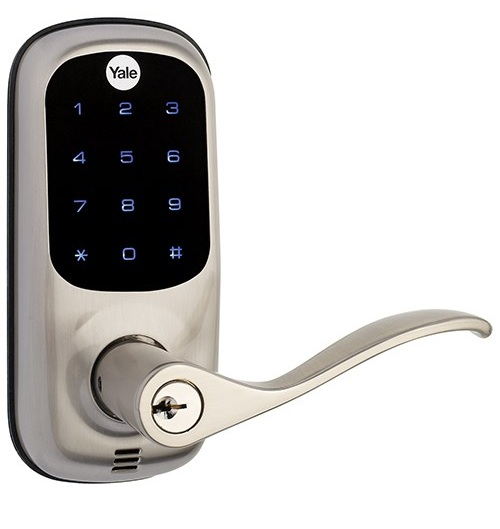
\includegraphics[scale=0.5]{figuras/cap3/yalerealliving.jpg}\\
  Fonte: Adaptado de \cite{yalerealliving}.
  \label{yalerealliving}
  \end{center}
  \end{figure}


 \subsection{Fechadura digital com senha e controle remoto}

 Além de senha, a fechadura digital \textbf{Milre Advance Control Tech 6300} (apresentada na Figura~\ref{milre6300}) pode ser controlada por controle remoto. Essa fechadura possui teclado \textit{touch screen} iluminado, dispositivo anti-hacker, travamento automático da porta, alarme contra invasão e sensor térmico interno que libera a porta em caso de incêndio. Com custo médio de R{\$} $1.183,00$ (mil cento e oitenta e três reais), a Control Tech 6300 é um modelo de embutir com maçaneta e liberação através de senha numérica ou chave digital. Esse dispositivo permite o cadastro de 8 senhas e até 45 chaves digitais, mas acompanha somente 4 chaves digitais; é alimentado com 4 pilhas tipo AA, com carga suficiente para durar até um ano, considerando uma média de utilização de vinte aberturas por dia, e emite aviso de esgotamento ao termino de carga das  pilhas \cite{milre6300}.

  \begin{figure}[!ht]
  \begin{center}
  \caption{Fechadura eletrônica Milre Advance Control Tech 6300R.}
  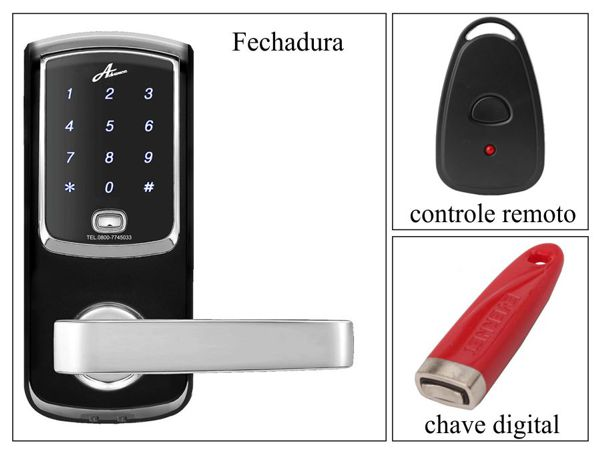
\includegraphics[scale=0.6]{figuras/cap3/milre6300.jpg}\\
  Fonte: Adaptado de \cite{milre6300}.
  \label{milre6300}
  \end{center}
  \end{figure}


 \subsection{Fechadura digital inteligente com sensor infravermelho}

 A \textbf{Samsung SHS-3321} (mostrada na Figura~\ref{samsungshs3321}) é uma fechadura digital sem maçaneta que possui leitor de cartões de $13,56$ MHz, com capacidade de registro de até setenta usuários, os quais podem obter acesso ao local protegido utilizando cartões de uso exclusivo ou códigos de segurança. Essa fechadura também dispõe de teclado numérico \textit{touch screen}; é alimentada com 4 pilhas tipo AA que duram cerca de um ano, com uma média de utilização de dez aberturas por dia; detecta a presença de possíveis intrusos por meio de sensor infravermelho; e pode ser adquirida por um valor médio de R{\$} $1.442,00$ (mil quatrocentos e quarenta e dois reais) \cite{samsungshs3321}.


  \begin{figure}[!ht]
  \begin{center}
  \caption{Fechadura inteligente Samsung SHS-3321.}
  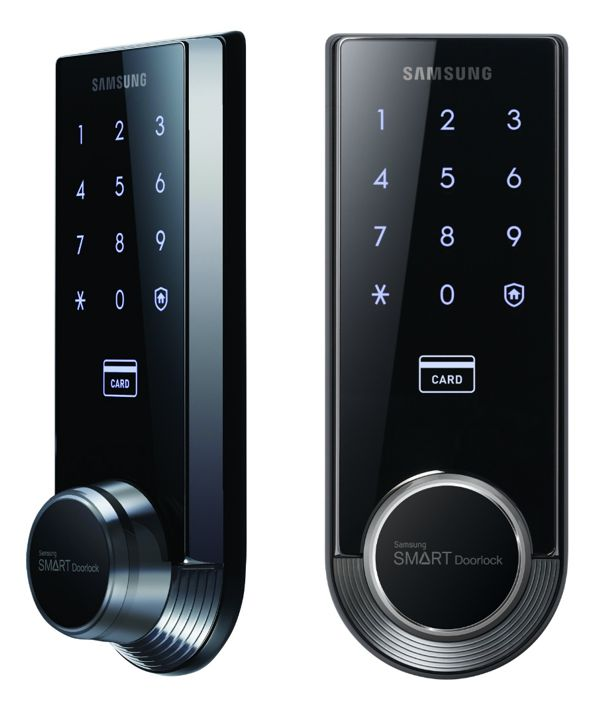
\includegraphics[scale=0.35]{figuras/cap3/samsungshs3321.jpg}\\
  Fonte: Adaptado de \cite{samsungshs3321}.
  \label{samsungshs3321}
  \end{center}
  \end{figure}


 \subsection{Fechadura biométrica com relatório de acessos}

 Utilizando biometria e senha, a \textbf{L7000} (mostrada Figura~\ref{zktecol7000}), é uma fechadura compacta que engloba múltiplas funcionalidades. Além da impressão digital e de senhas, ela permite o uso de chaves para controlar o acesso ao ambiente em que é instalada. A \textbf{L7000} possui as seguintes características: é um dispositivo com conexão USB que possibilita a troca de dados com o computador para gerar relatório utilizando o \textit{software} fornecido pelo fabricante; é capaz de armazenar 500 digitais, 100 senhas e o registro de 30.000 acessos; permite programar horários específicos de acesso para cada usuário; dispara alarme tentativa de acesso não autorizada; opera com 4 pilhas comuns (AA) que duram aproximadamente 4.000 aberturas; possui \textit{display} de diodo orgânico emissor de luz (\textit{organic light-emitting diode} -- OLED), que exibe a carga das baterias e alerta quanto a necessidade de troca \cite{zktecol7000}; e custa em média R{\$} $1.490,00$ (mil quatrocentos e noventa reais).

  \begin{figure}[!ht]
  \begin{center}
  \caption{Fechadura biométrica  ZKTeco L7000}
  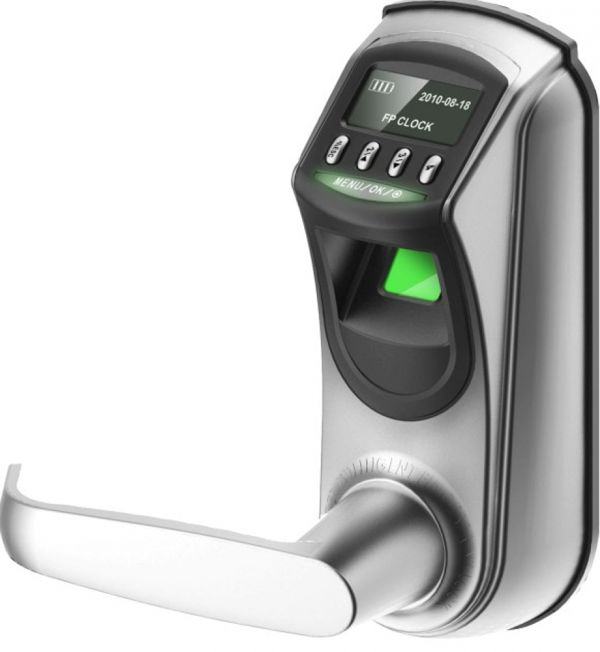
\includegraphics[scale=1]{figuras/cap3/zktecol7000.jpg}\\
  Fonte: Adaptado de \cite{zktecol7000}.
  \label{zktecol7000}
  \end{center}
  \end{figure}
  

 \subsection{Fechadura inteligente com autenticação dupla}

 Uma das mais caras opções de fechadura biométrica, a \textbf{Samsung SHS-P718} (mostrada na Figura~\ref{samsungshsp718}) pode custar até R{\$} $3.217,00$ (três mil duzentos e dezessete reais). Trata-se de um produto com design sofisticado e autenticação dupla que solicita a impressão digital e senha para abertura da porta. Tem capacidade para registrar até 100 impressões digitais, 30 usuários com senha ou cartão RFID; sua alimentação depende de 8 pilhas AA, suficientes para durarem aproximadamente um ano; inclui também sensor de movimentos infravermelho, alarme de incêndio, sons operacionais e mensagem de voz \cite{samsungshsp718}.

  \begin{figure}[!ht]
  \begin{center}
  \caption{Fechadura inteligente Samsung SHS-P718}
  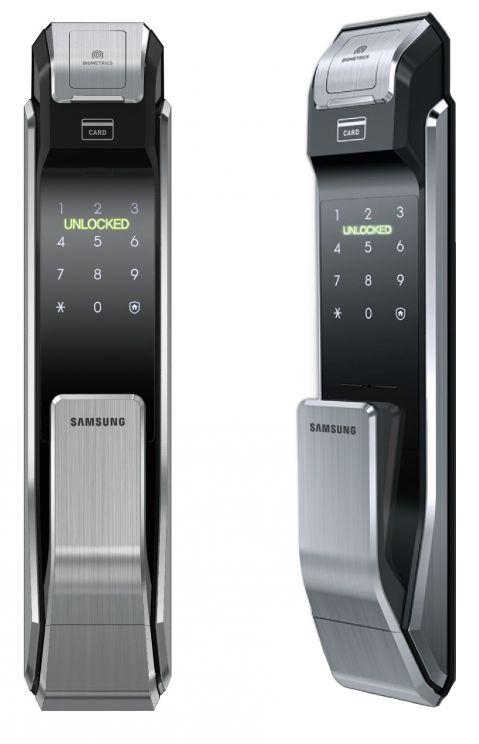
\includegraphics[scale=1.3]{figuras/cap3/samsungshsp718.jpg}\\
  Fonte: Adaptado de \cite{samsungshsp718}.
  \label{samsungshsp718}
  \end{center}
  \end{figure}


 \subsection{Controlador de acesso biométrico\label{F7}}

 O propósito de utilização do dispositivo de controle de acesso \textbf{F7} (Figura~\ref{zktecof7}), vai além de ambiente residenciais, podendo ser instalado em qualquer tipo de portaria e empresa. É um dos produtos \textit{off-line} (não depende de conexão à rede de computador), com maior capacidade de usuários. O \textbf{F7} é capaz de armazenar dados de acesso (50.000 registros) e cadastrar a impressão digital de 2.200 usuários, os quais podem utilizar a biometria, senha ou ambos. Além disso, o equipamento tem saída para sirene, sensor de porta, controle de porta, fechaduras elétricas e eletrônicas, também oferece saídas RS232, RS485 e conexão Ethernet (comunicação TCP/IP) que permite a conexão com um computador ou rede de computador para o gerenciamento dos dados armazenados, como mostra o diagrama da Figura~\ref{diagrama_zktecof7}. O aparelho é alimentado via fonte $12$ V DC e acompanha uma bateria extra que pode durar até 15 horas, dependendo do uso \cite{zktecof7}. Esse produto custa em média R{\$} $1.357,00$ (mil trezentos e cinquenta e sete reais), é distribuído por diversos fornecedores no Brasil e pode ser facilmente encontrado em lojas físicas e \textit{e-commerce}. 
 
 



  \begin{figure}[!ht]
  \begin{center}
  \caption{Controlador de acesso biométrico ZKTeco F7}
  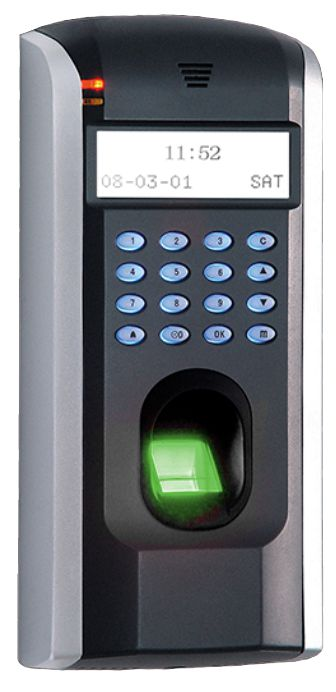
\includegraphics[scale=0.3]{figuras/cap3/zktecof7.jpg}\\
  Fonte: Adaptado de \cite{zktecof7}.
  \label{zktecof7}
  \end{center}
  \end{figure}


  \begin{figure}[!ht]
  \begin{center}
  \caption{Diagrama de conexão do controlador de acesso ZKTeco F7.}
  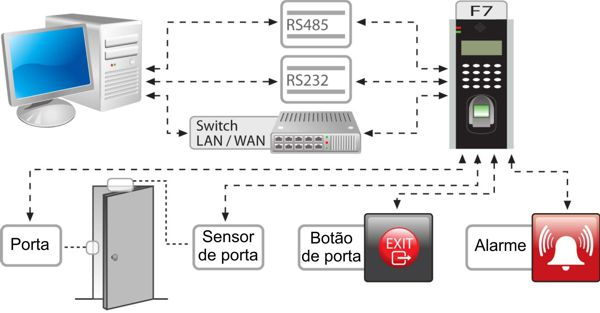
\includegraphics[scale=0.8]{figuras/cap3/diagrama_zktecof7.jpg}\\
  Fonte: Adaptado de \cite{zktecof7}.
  \label{diagrama_zktecof7}
  \end{center}
  \end{figure}


 \subsection{Controlador de acesso multifuncional}

 O controlador de acesso \textbf{iDAccess} (mostrado Figura~\ref{idaccess}), é voltado para o controle de ponto de funcionários em ambientes que possuem um grande volume de usuários. O aparelho gera relatório de acesso, faz a identificação de pessoas utilizando a impressão digital, cartão de proximidade e senha, e pode operar no modo \textit{stand alone} ou \textit{on-line}. No modo \textit{stand alone}, o equipamento é capaz de armazenar mais de 2.000 digitais e os dados de acesso podem ser consultados através de \textit{software} web embarcado. Em modo \textit{on-line}, o \textbf{iDAccess} conecta-se à rede de computador via porta Ethernet 10/100 Mbps. O dispositivo pode ser integrado a um sistema (servidor), oferecido pelo fabricante, que aumenta a sua capacidade de armazenamento para mais de 100.000 digitais e 1.000.000 de registros. Esse aparelho é alimentado por uma fonte externa de $12$ V, possui central de alarme, aceita módulo de conexão Wi-fi e GPS (opcionais). Além disso, esse sistema dispõe de serviço opcionais para monitoramento, sincronização e backup de dados em nuvem \cite{idaccess}. 

 O iDAccess se destaca pela capacidade de armazenamento de dados e registro de usuários em modo \textit{off-line}, e também pela possibilidade de expansão dessa capacidade com a integração de um sistema \textit{on-line}, além de estar na mesma faixa de preço de produtos com capacidade inferior, em média R{\$} $1.645,00$ (mil seiscentos e quarenta e cinco reais).

  \begin{figure}[!ht]
  \begin{center}
  \caption{Controlador de acesso multifuncional iDAccess.}
  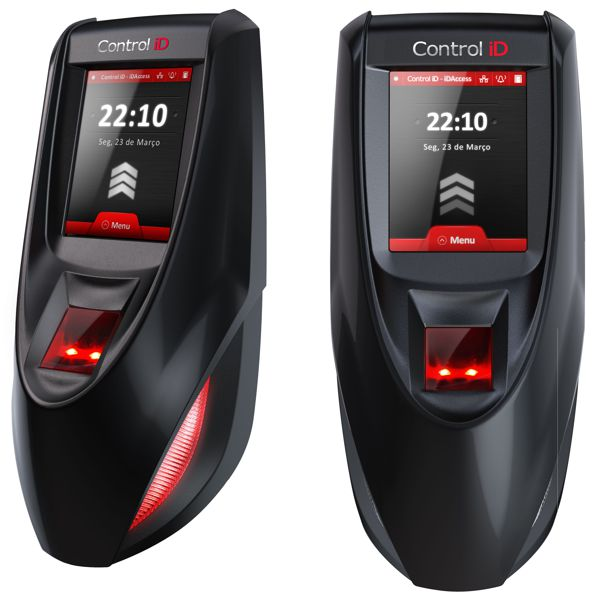
\includegraphics[scale=0.4]{figuras/cap3/idaccess.jpg}\\
  Fonte: Adaptado de \cite{idaccess}.
  \label{idaccess}
  \end{center}
  \end{figure}


 \subsection{Relógio de ponto biométrico}

 O aparelho mostrado na Figura~\ref{fingerprinttimeattendance}, conhecido apenas como \textit{Fingerprint time Attendance} em e-commerce estrangeiro ou como Relógio de Ponto Biométrico, no Brasil, é um produto chinês com poucas informações oficiais, fornecido por diferentes representantes, isto é, diferentes fabricantes produzem ou revendem um dispositivo utilizando o mesmo design, porém cada um com sua marca. No geral, esse produto é um relógio de ponto que funciona com impressão digital ou senha; tem capacidade para 600 impressões digitais e 150.000 registros, que podem ser exportados para um \textit{pen drive} em um arquivo no formato de planilha; é alimentado por fonte externa, não possui bateria \cite{fingerprinttimeattendance}; e tem um custo relativamente baixo, R{\$} 195,00 (cento e noventa e cinco reais).

  \begin{figure}[!ht]
  \begin{center}
  \caption{Relógio de ponto biométrico}
  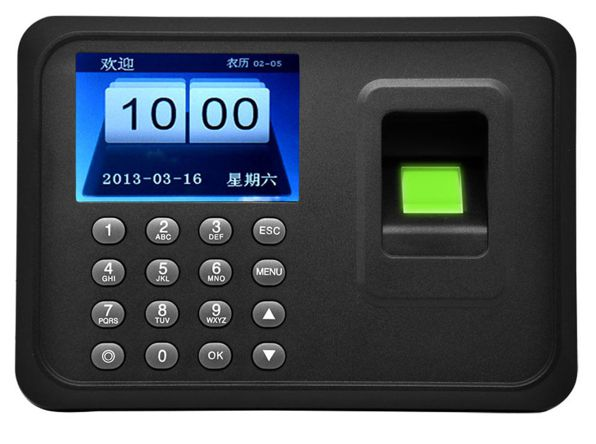
\includegraphics[scale=0.3]{figuras/cap3/fingerprinttimeattendance.jpg}\\
  Fonte: Adaptado de \cite{fingerprinttimeattendance}.
  \label{fingerprinttimeattendance}
  \end{center}
  \end{figure}
  
  
 \subsection{Leitores biométricos para sistemas de larga escala}
  
  
  \begin{figure}[!ht]
  \begin{center}
  \caption{Leitor de impressão digital U.are.U 4500}
  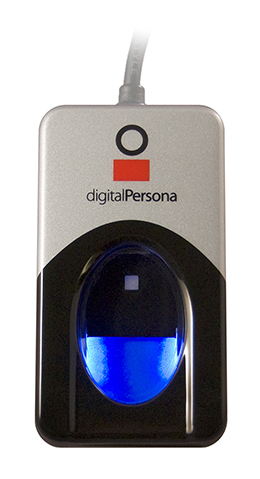
\includegraphics[scale=0.4]{figuras/cap3/uareu4500digitalpersona.jpg}\\
  Fonte: Adaptado de \cite{uareu4500digitalpersona}.
  \label{uareu4500digitalpersona}
  \end{center}
  \end{figure}
  
  
  No mercado de segurança são oferecidos uma gama de produtos eletrônicos para controle de acesso. A maioria desses produtos são fechaduras eletrônicas e relógios de ponto que utilizam tecnologia baseada em biometria. Além desse tipo de produto, existem empresas que oferecem sensores biométricos para aplicações em sistemas de larga escala, como por exemplo, o leitor de impressão digital Digital Persona U.are.U 4500\cite{uareu4500digitalpersona} (apresentado na Figura~\ref{uareu4500digitalpersona}), fabricado pela empresa Crossmatch. A Crossmatch fornece dispositivos para a empresa americana Microsoft e a brasileira Computer Digital. Esses sensores podem ser manipulados através de SDKs disponibilizados pelo fabricante ou por projetos \textit{opensource}. Também podem ser empregados em aplicações desenvolvidas pelo próprio usuário. 
  Um U.are.U 4500 pode ser adquirido por cerca de R{\$} $415,00$ (quatro centos e quinze reais) e a limitação de usuários e armazenamento de dados de acesso fica por conta das especificações do sistemas em que ele for instalado, pois essas limitações dependem de aspectos, como projeto de banco de dados, algoritmo de reconhecimento da característica biométrica e capacidade de processamento da máquina que executa o sistema.

 
 As soluções de mercado podem ser divididas em duas grandes categorias, \textit{on-line} e \textit{off-line}. As soluções de natureza \textit{on-line} normalmente custam mais caro e constituem sistemas integrados que podem reconhecer milhares de usuários, os quais podem estar situados em diferentes localizações ou pertencer a instituições distintas. Enquanto que maioria dos produtos \textit{off-line} não garantem a segurança dos dados bioméricos e registro de acesso, pois o propósito de grande parte desses produtos é o controle simples de acesso físico, sem um interesse maior no gerenciamento de dados. Essas soluções são proprietárias e o usuário não tem acesso ao dispositivo a nível de desenvolvimento, isto é, o usuário não pode fazer modificações no \textit{hardware} ou \textit{software}.


 \section{Considerações}

 O objetivo das propostas acadêmicas é oferecer soluções de controle de acesso visando o baixo custo para aplicações específicas, como o controle de frequência de alunos, controle de acesso residencial e estudos de caso, por exemplo. A maioria desses trabalhos visa beneficiar a comunidade acadêmica na qual são desenvolvidos ou a sociedade em geral, através da elaboração de projetos que atendem necessidades ainda não atendidas pela indústria. Enquanto que as soluções de mercado têm um custo de aquisição relativamente elevado e são soluções genéricas de controle de acesso que têm como objetivo oferecer mais funcionalidade, sofisticação e automatização para o usuário.
 
 
 
 
\chapter{Solução proposta\label{cap:desenvolvimento}}

\section{Introdução}

Neste capítulo é apresentada a solução proposta para controle de acesso físico utilizando tecnologia de biometria e uma aplicação web. Essa solução trata-se de um sistema eletrônico baseado em \textit{hardware} e \textit{software} livre. Tal sistema utiliza a impressão digital como característica biométrica para a autenticação de usuários. A autenticação de impressões digitais é um processo de segurança utilizado em ambientes que necessitam do controle de entrada de pessoas, a fim de restringir o acesso às pessoas autorizadas. O sistema em questão é batizado de Setfinger. Esse sistema é composto por dois elementos: um cliente e um servidor. O cliente é o aparelho responsável pela interface com o usuário, leitura de impressões digitais e controle de fechadura eletrônica (fecho elétrico). O servidor propriamente dito, aqui chamado de Setserver, é a máquina na qual devem ser instalados os serviços de conexão TCP, banco de dados e plataforma web. Portanto, o Setserver é composto por um servidor TCP baseado em node.js, um banco de dados Mysql e uma plataforma de gerenciamento web. O servidor TCP é responsável por criar uma conexão do tipo TCP, manter a comunicação com o cliente e gravar informações no banco de dados, de acordo com os comandos enviados pelo cliente. O banco de dados armazena os cadastros e os registro de acesso dos usuários. Por fim, a página web provê o gerenciamento dos dados mantidos no banco de dados, tais como, atualização e exclusão de cadastros, consulta da frequência de usuários, em tabelas ou gráficos, e a obtenção de relatórios. O cliente e o servidor se comunicam via conexão TCP/IP, em uma rede de computador, como ilustrado na Figura~\ref{rede_setfinger}. A seguir, são apresentados os objetivos do sistema Setfinger.

\begin{figure}[!ht]
  \begin{center}
  \caption{Sistema Setfinger instalado em uma rede local - Exemplificação de comunicação entre o aparelho Setfinger (cliente) e o servidor, através de uma Rede local.}
  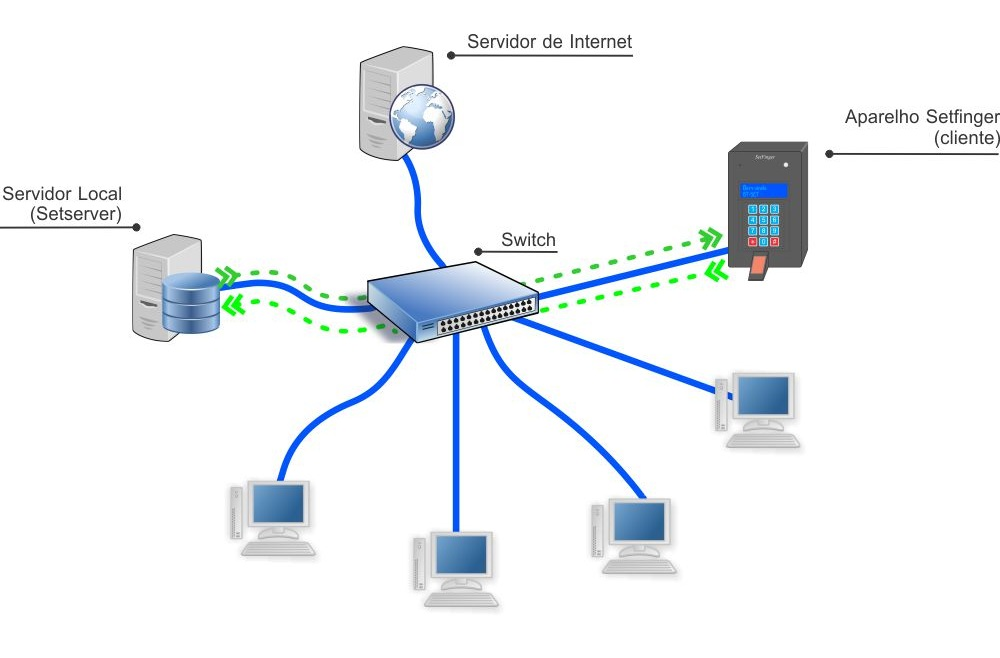
\includegraphics[scale=0.6]{figuras/cap4/rede_setfinger.jpg}\\
  Fonte: Elaborada pelo autor.
  \label{rede_setfinger}
  \end{center}
  \end{figure}

\section{Objetivos do sistema Setfinger\label{objetivos_sf}}

O sistema Setfinger foi desenvolvido no Grupo Servidor de Estação de Trabalho (GT-SET) do Centro de Tecnologia da Informação e Comunicação (CTIC) da Universidade Federal do Pará (UFPA). Essa solução foi elaborada com o propósito de atender as demandas de controle de acesso físico interno da UFPA. Os principais objetivos definidos na elaboração do projeto Setfinger são:

\nomenclature{GT-SET}{Grupo Servidor de Estação de Trabalho}
\nomenclature{CTIC}{Centro de Tecnologia da Informação e Comunicação}



\begin{itemize}

\item Substituir o uso de chaves por biometria

O espaço interno do CTIC é dividido em salas, porém o acesso ao prédio é livre para atendimento ao público. Desta forma, a porta de cada sala deveria permanecer trancada para evitar que visitantes tenham acesso direto a elas. No entanto, a utilização de chaves para trancar e destrancar a porta repetidas vezes, pode se tornar um processo incômodo para os usuários. Sendo assim, a utilização de tecnologia biométrica torna-se um processo mais rápido e prático, uma vez que não há a possibilidade do usuário esquecer ou perder a chave de acesso (biometria). 


\item Aumentar a segurança de usuários e bens

Garantindo a restrição de acesso para usuários não autorizados, pode-se proporcionar maior segurança para os usuários e evitar possíveis incidentes envolvendo pessoas não integrantes às salas.


\item Registrar o acesso de bolsistas e servidores para controle de ponto

O uso de um sistema digital torna mais eficiente o registro de acesso de pessoas em um determinado local. Isso automatiza o processo de controle de ponto, garante maior segurança às informações registradas e torna os dados mais acessíveis para supervisores e supervisionados.  


\item Gerar relatório de acesso

Através dos registros de acesso dos usuários, pode-se gerar relatório para avaliação ou comprovação de frequência.


\item Redução de custos

Na porta de entrada principal do CTIC é utilizado um dispositivo de controle de acesso semelhante ao modelo F7, apresentado na Seção~\ref{F7}. O objetivo do CTIC é que cada sala disponha de um aparelho de controle de acesso biométrico. O ideal seria que, além do CTIC, outros espaços da UFPA contassem com esse tipo de controle, porém esse dispositivo foi adquirido pelo valor de R\$ $2.400,00$ (dois mil e quatrocentos reais). Esse valor representa um custo alto para a UFPA. Desta forma, há a necessidade de uma solução de custo reduzido, em relação as soluções de mercado, e com licença livre para que o próprio usuário (administrador) possa fazer a manutenção do sistema.

\end{itemize}

\section{Hardware}

O principal dispositivo utilizado no conjunto de \textit{hardware} do sistema Setfinger é o Arduino Mega, uma ferramenta de prototipagem eletrônica \textit{open-source} que tem sido amplamente utilizada no ambiente acadêmico para o desenvolvimento do conhecimento de eletrônica, \textit{hardware} e sistemas embarcados. Essa plataforma permite o desenvolvimento de soluções para inúmeros tipos de aplicações e problemas, podendo ser integrado a sensores e outros componentes que ampliam sua capacidade de interação. Em comparação a outras opções de \textit{hardware} microcontrolado, o Arduino é um dos mais populares, possui grande oferta no mercado, tem custo relativamente baixo e programação de alto nível. Além disso, a comunidade do Arduino é composta por um número grande de desenvolvedores, fóruns de discussões e materiais que facilitam o uso da placa para a elaboração de projetos simples ou complexos. Esses foram os principais aspectos que motivaram a escolha do Arduino para a elaboração do módulo de \textit{hardware} aqui proposto. Além disso, o ambiente de desenvolvimento em que a solução proposta é projetada pratica uma política de criação de soluções baseadas na filosofia \textit{open source}. Por isso, o principal critério avaliado na escolha dos recursos utilizados na execução deste projeto é a licença \textit{open-source}. Além do Arduino, são utilizados componentes selecionados de acordo com a sua popularidade, compatibilidade com o microcontrolador, suporte, custo e oferta no mercado, pois alguns componentes são escassos no mercado brasileiro, possuem preços elevados e não apresentam documentação. Portanto, nesta seção é apresentado o \textit{hardware} do aparelho Setfinger proposto, bem como o material e as técnicas utilizadas no seu desenvolvimento, e o papel de cada um dos elementos que o compõem.


\subsection{\textit{Hardware} Setfinger proposto \label{hardware_setfingerproposto}}

De acordo com os objetivos definidos na Seção~\ref{objetivos_sf}, é proposto um aparelho biométrico com \textit{hardware} baseado em plataforma Arduino. Tal aparelho é dividido em dois módulos: um módulo de interface com o usuário e um módulo de \textit{hardware} interno (veja a Figura~\ref{setfinger_modulos}). O módulo de interface com o usuário permite a interação do usuário com o sistema Setfinger. Esse módulo é composto por um display LCD, um teclado matricial e um leitor de impressões digitais. O módulo interno é composto por um Arduino Mega 2560, um ethernet shield W5100 e uma placa de integração de componentes, denominada Setshield, a qual é responsável por conectar ao Arduino os componentes apresentados na Tabela~\ref{tabela_componentes}. A placa Setshield presente no módulo de \textit{hardware} interno, contém um relé que deve ser associado em série ao fecho elétrico que controlará a abertura da porta que dá acesso ao ambiente a ser controlado. Portanto, é necessária a divisão do aparelho em dois módulos para evitar, em casos de arrombamento do aparelho, que usuários mal intencionados tenham acesso a esse relé.

Além do \textit{hardware} proposto aqui, são apresentadas outras duas versões de \textit{hardware} no Apêndice~\ref{hardware_1.0} e Apêndice~\ref{hardware_2.0}. No entanto, a versão proposta apresenta um projeto de \textit{hardware} otimizado, em relação as demais versões, pois nessa versão de \textit{hardware} o circuito da placa Setshield apresenta um layout menor e há uma redução na quantidade de fios necessários para conectar os componentes ao Arduino.

Na Figura~\ref{diagrama_hardware}, é apresentado o diagrama de blocos que representa o layout do \textit{hardware} do Setfinger proposto. A partir desse diagrama é possível identificar todos os componentes de \textit{hardware} que integram o sistema Setfinger, e compreender a relação entre eles.

\begin{figure}[!t]
  \begin{center}
  \caption{Aparelho Setfinger - à esquerda da imagem é mostrado o módulo de interface com o usuário e à direita da imagem é mostrado o módulo de \textit{hardware} que deve ser instalado fora do alcance do usuário, de preferência no interior da sala a ser controlada. O módulo de \textit{hardware} interno é mostrado sem nenhuma proteção (carcaça), mas deve ser embutido em um gabinete plástico.}
  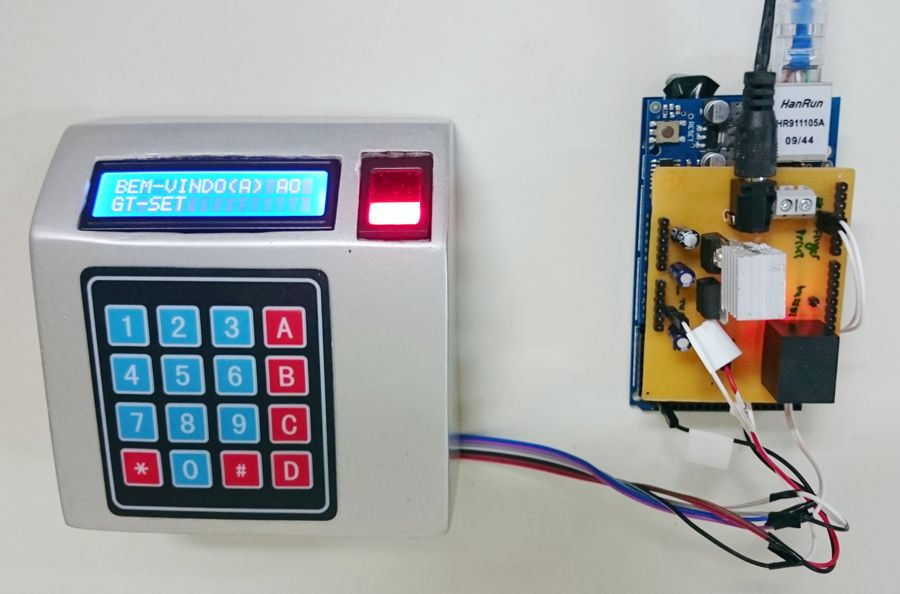
\includegraphics[scale=0.4]{figuras/cap4/setfinger_modulos.jpg}\\
  Fonte: Elaborada pelo autor.
  \label{setfinger_modulos}
  \end{center}
  \end{figure}
  
  
  
  
  \begin{table}[]
\centering
\caption{Tabela de componentes conectados ao Arduino através da placa Setshield.}
\label{tabela_componentes}
\begin{tabular}{ll}
\hline
%\multicolumn define as configurações de alinhamento e exibição de colunas
\multicolumn{1}{c}{\textbf{Quantidade}} & \multicolumn{1}{c}{\textbf{Componentes}} \\ \hline\hline
\multicolumn{1}{c}{1} & Relé CONT: $10$ A $125$ V AC/ COIL: $5$ V DC\\ \hline
\multicolumn{1}{c}{3} & Resistor $4.6$ k$\Omega$ \\ \hline
\multicolumn{1}{c}{3} & Resistor $1$ k$\Omega$\\ \hline
\multicolumn{1}{c}{2} & Capacitor $47 \mu$ F $16$ V\\ \hline
\multicolumn{1}{c}{1} & Capacitor $100 \mu$ F $16$ V\\ \hline
\multicolumn{1}{c}{1} & Regulador de tensão L7809\\ \hline
\multicolumn{1}{c}{1} & Regulador de tensão L7805\\ \hline
\multicolumn{1}{c}{1} & Conector Jack P4 para placa $2,1$ mm\\ \hline
\multicolumn{1}{c}{1} & Borne para placa (com parafuso)\\ \hline
\multicolumn{1}{c}{1} & Sensor Fingerprint ZFM-20\\ \hline
\multicolumn{1}{c}{1} & Display LCD 16x2 5V\\ \hline
\multicolumn{1}{c}{1} & Teclado matricial\\ \hline


\end{tabular}
\end{table}

  
  
  
\begin{figure}[!t]
  \begin{center}
  \caption{Diagrama de \textit{hardware} do aparelho Setfinger.}
  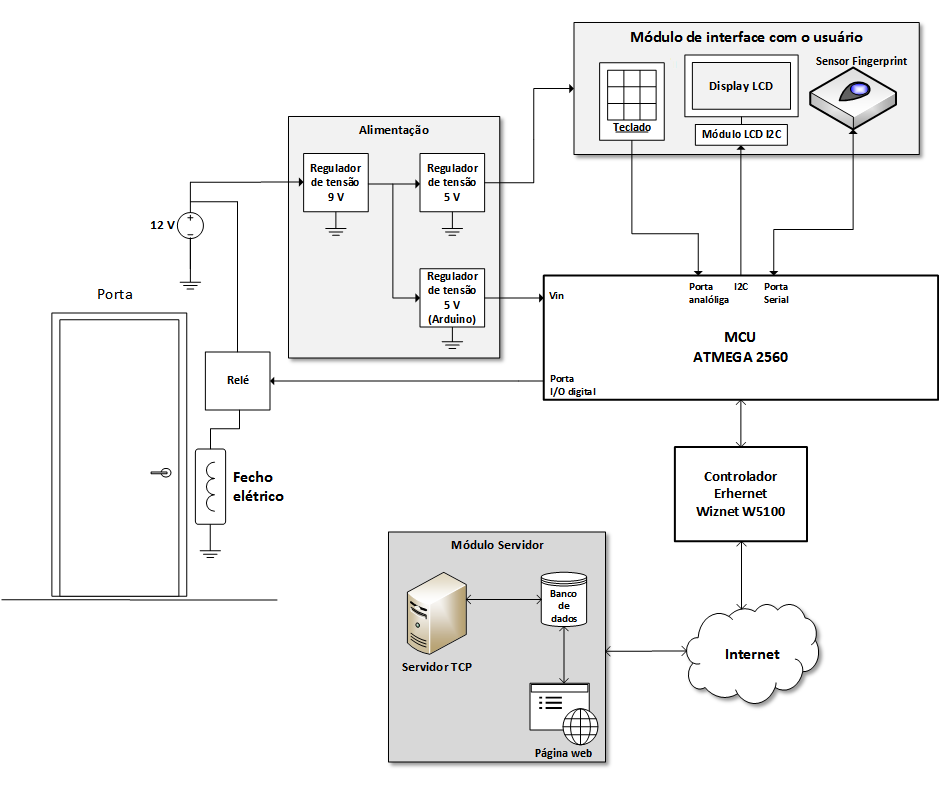
\includegraphics[scale=0.6]{figuras/cap4/diagrama_hardware.png}\\
  Fonte: Elaborada pelo autor.
  \label{diagrama_hardware}
  \end{center}
  \end{figure}
  
  
  
 A seguir, são descritas a atuação de cada elemento presente no diagrama de \textit{hardware} mostrado na Figura~\ref{diagrama_hardware}, assim como, suas características e funcionamento. Além disso, são apresentadas considerações importantes sobre a pinagem dos componentes, pois os barramentos de comunicação serial, como I2C, SPI, TTL, ou saídas digitais com sinal PWM, estão presentes em pinos específicos da Unidade de Microcontrolador (\textit{microcontroller unit} -- MCU). Portanto, a conexão de cada dispositivo deve ser realizada de acordo com o seu tipo de comunicação. Normalmente, a pinagem adequada para cada componente é informada pelo fabricante.
 
 \nomenclature{MCU}{Microcontroller Unit}
 
\begin{itemize}
    
    \item Fecho elétrico
    
    O fecho elétrico é um dispositivo instalado junto a fechadura da porta e pode ser controlado eletronicamente. Os fechos elétricos utilizados neste trabalho operam sob uma tensão de $12$ V. Esses dispositivos possuem um solenoide em seu interior. Ao ser energizado, o solenoide move uma pequena peça que destrava a fechadura e permite a abertura da porta. Alguns modelos de fecho elétrico possuem um mecanismo chamado de memória, com esse mecanismo basta que o solenoide seja energizado por um instante e a fechadura permanecerá destravada até que a porta seja aberta. Nos mecanismos sem memória, a fechadura só permanece destravada enquanto o solenoide estiver sendo alimentado \cite{tobias2015illustrated, norman2011electronic}.   
    
    \item Relé
    
    O relé é o componente responsável por permitir ou interromper a passagem de corrente no circuito em que o fecho elétrico é alimentado. O relé está conectado em série com o fecho elétrico e funciona como uma chave.
    
    \item Alimentação
    
    Nesta versão de \textit{hardware} é utilizada somente uma fonte de alimentação. A mesma fonte utilizada para alimentar o fecho elétrico, foi utilizada para alimentar o aparelho Setfinger. O microcontrolador (MCU - Atmega 2560), opera sob uma tensão de $5$ V e a placa Arduino, na qual a MCU é instalada, possui um regulador de $5$ V (AMS 1117). No entanto, foi adicionado um regulador extra de $5$ V para alimentar somente o teclado, display LCD e sensor Fingerprint. Para alimentar os dois reguladores de $5$ V foi adicionado um regulador de $9$ V. Os dois reguladores foram adicionados, a fim de distribuir o aquecimento entre os reguladores e reduzir o aquecimento excessivo sobre o regulador de $5$ V da placa Arduino, que ocorre devido ao elevado consumo de corrente do controlador ethernet.  
    
    \item Display LCD
    
    O Display LCD é um dispositivo de saída que possui 2 linhas de 16 caracteres, responsável por exibir as mensagens de instrução aos usuários. O Display LCD possui 6 pinos de dados, 4 pinos GND e 2 
    pinos 5V. Portanto, são necessários 12 fios para conectar o display ao Arduino. Essa quantidade de fios pode ser reduzida através do uso de um módulo I2C, que emprega somente dois fios de dados e dois fios de alimentação. O módulo é soldado diretamente aos pinos do Display LCD e desse módulo saem apenas duas vias de dados e duas vias de alimentação. 

    \item Teclado matricial
    
    O teclado matricial é um componente utilizado como entrada. Neste trabalho, as teclas $1$ e $2$ foram associadas às duas opções do menu de administrador (1 - entrar e 2 - cadastrar). Assim, as teclas podem ser utilizadas para selecionar opções de menu ou senhas, o que não é o caso dessa aplicação, pois não há opção de senha para o usuário. Apesar de serem utilizadas somente duas teclas nesse projeto, que poderiam ser substituídas por dois botões, o teclado completo permanece no projeto, pois havendo a necessidade de senha, a mudança pode simplesmente ser feita apenas a nível de \textit{software}. 
    
    O teclado matricial 4x3 possui somente 7 vias de conexão, sendo 4 vias referentes as linhas e 3 referentes as colunas. Essa quantidade de conexões pode ser reduzida para 3 vias, através de um circuito divisor de tensão, conhecido como \textit{one wire keypad} \cite{arduinocc_onewirekeypad}, que utiliza 2 vias para alimentação e uma via de dados (veja a Figura~\ref{onewirekeypad}).

    \begin{figure}[!t]
    \begin{center}
    \caption{Esquema de resistores para a redução do numero de pinos digitais utilizados por um teclado matricial 4x3 no Arduino.}
    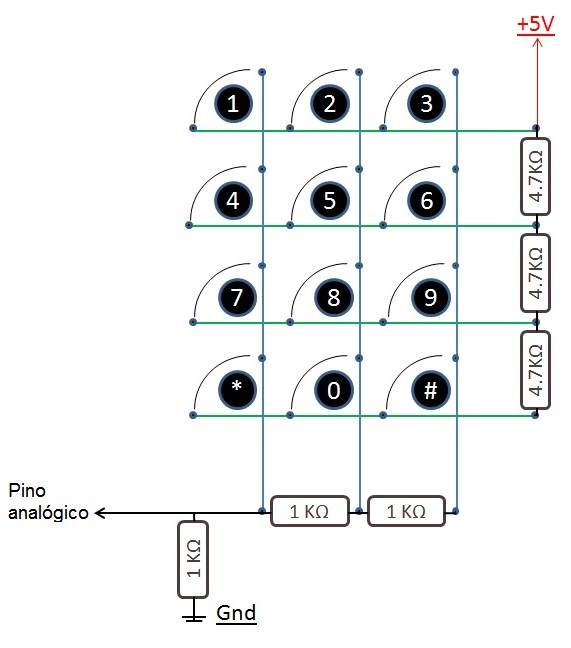
\includegraphics[scale=0.55]{figuras/cap4/onewirekeypad.jpg}\\
    Fonte: Adaptado de \cite{arduinocc_onewirekeypad}.
    \label{onewirekeypad}
    \end{center}
    \end{figure}
    
    
    \item Sensor Fingerprint
    
    O sensor Fingerprint faz a leitura de impressões digitais dos usuários. O processamento digital que envolve as operações de leitura e reconhecimento de impressões digitais, e o armazenamento das digitais são realizados no próprio sensor biométrico. Desta forma, são enviados comandos para que o sensor execute as ações desejadas. No total, o sensor possui apenas 4 pinos para conexão, 2 de alimentação e 2 de dados TTL serial (TX e RX). Portanto, o RX e TX do sensor devem ser conectados no TX e RX da MCU, respectivamente. Apesar de o Arduino Mega possuir somente 4 portas seriais, é possível conectar o sensor em outros pinos digitais que não dispõem de porta serial, através da criação de portas seriais virtuais. 
    
    \item MCU
    
    A MCU utilizada neste projeto é um microcontrolador Atmega 2560, responsável pelo processamento e manipulação dos dispositivos de entrada e saída no aparelho Setfinger.
    
    \item Controlador Ethernet
    
    O controlador ethernet provê a conexão do aparelho Setfinger à internet, assim estabelecendo a comunicação entre o aparelho Setfinger e o módulo servidor. O controlador ethernet é conectado a MCU através de comunicação SPI (\textit{Serial Peripheral Interface}), uma interface serial síncrona desenvolvido pela Motorola que permite a comunicação entre microcontroladores e periféricos, em comunicação de curta distância. Esse padrão pode ser utilizado em aplicações com cartões SD, \textit{displays} LCD, sensores, módulos RTC e até mesmo outros microcontroladores \cite{catsoulis2005designing, ganssle2007embedded, chattopadhyay2013embedded}. É importante ressaltar que no Arduino o controlador ethernet é conectado através do conjunto de pinos denominado \textit{ICSP}. Quando conectado ao Arduino Uno, os pinos 10, 11, 12 e 13 não podem ser utilizados. Se conectado ao Arduino Mega, os pinos 50, 51 e 52 não podem ser utilizados. Em ambos os casos os pinos citados não funcionarão para outras finalidades de I/O, pois são ocupados pela comunicação SPI (para mais detalhes, veja a documentação do Ethernet Shield \cite{ArduinoEthernetShield}).
    \nomenclature{I/O}{Entrada/saída (\textit{input/output})}
    
    \item Módulo Servidor
    
    O módulo servidor mantém as informações de controle de acesso dos usuários, estabelece a conexão com os clientes e disponibiliza o gerenciamentos de dados. Por se tratar de um módulo de \textit{software}, o servidor será abordado com mais detalhes na Seção~\ref{software}.
    
\end{itemize}
  
  Em relação as versões de \textit{hardware} apresentadas no Apêndice~\ref{hardware_1.0} e Apêndice~\ref{hardware_2.0}, a versão de \textit{hardware} proposta apresenta uma redução na quantidade de fios necessários para conectar o módulo de interface com o usuário ao módulo de \textit{hardware} interno (veja a Figura~\ref{circuit_setfinger_v3}). Essa redução de fios ocorre devido ao uso do circuito divisor de tensão \textit{one wire kaypad} e do módulo I2C em conjunto com o display LCD. A placa Setshield, mostrada na Figura~\ref{setshield_v3}, apresenta um resultado de PCB mais compacta em relação as versões 1.0 e 1.2. Além de tornar a placa Setshield mais compacta e reduzir a quantidade de fios, foi confeccionada uma carcaça menor e mais elegante para embutir os componentes de interface com o usuário (mostrada na Figura~\ref{setfinger_final}). Essa carcaça foi produzida em fibra de vidro com acabamento automotivo.
  
  O esquemático e o design da placa Setshield são produzidos no \textit{softwate} CadSoft Eagle 7.5.0 (veja o Apêndice~\ref{schematic_setshield} e Apêndice~\ref{board_setshield}).
  

\begin{figure}[!t]
  \begin{center}
  \caption{Circuito completo do \textit{hardware} Setfinger com todos os componentes conectados.}
  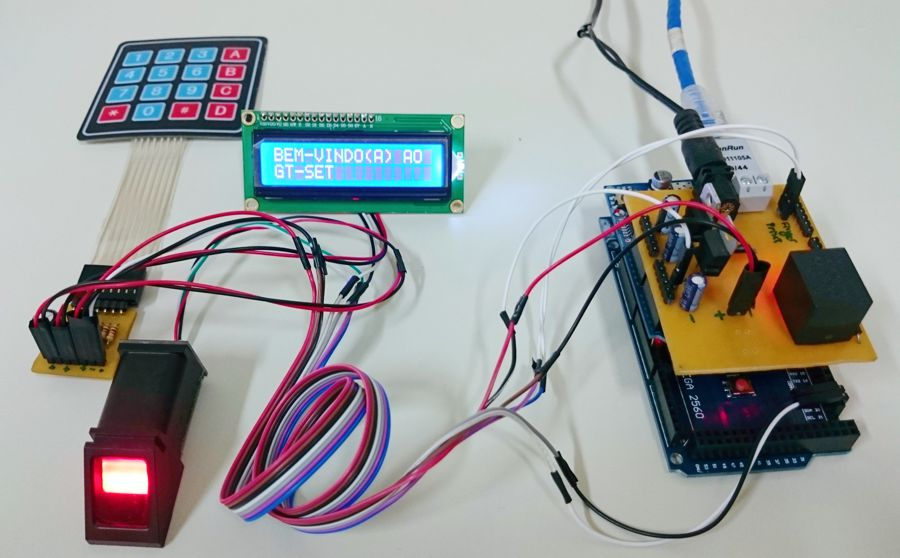
\includegraphics[scale=0.5]{figuras/cap4/circuit_setfinger_v3.jpg}\\
  Fonte: Elaborada pelo autor.
  \label{circuit_setfinger_v3}
  \end{center}
  \end{figure}
  
  
\begin{figure}[!t]
  \begin{center}
  \caption{Placa Setshield.}
  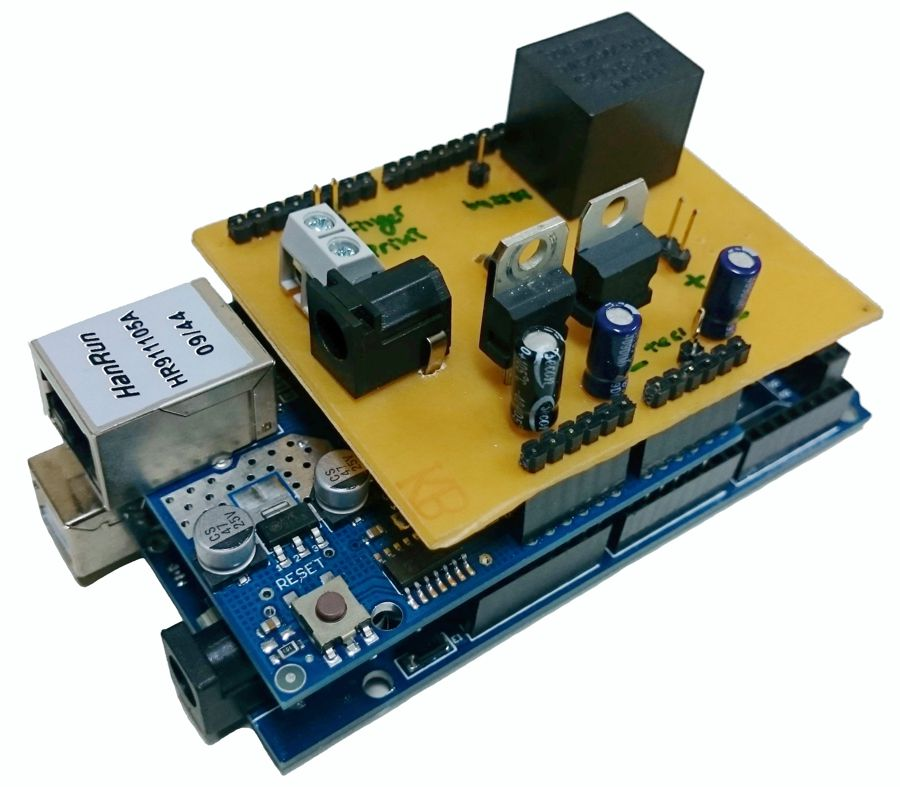
\includegraphics[scale=0.3]{figuras/cap4/setshield_v3.jpg}\\
  Fonte: Elaborada pelo autor.
  \label{setshield_v3}
  \end{center}
  \end{figure}
  

\begin{figure}[!t]
  \begin{center}
  \caption{\textit{Hardware} Setfinger -- módulo de interface com o usuário, composto por um display LCD, um leitor de impressões digitais e um teclado matricial do tipo membrana, embutidos em um gabinete de fibra de vidro. Este módulo deve ser instalado do lado externo do ambiente a ser controlado e próximo a porta}
  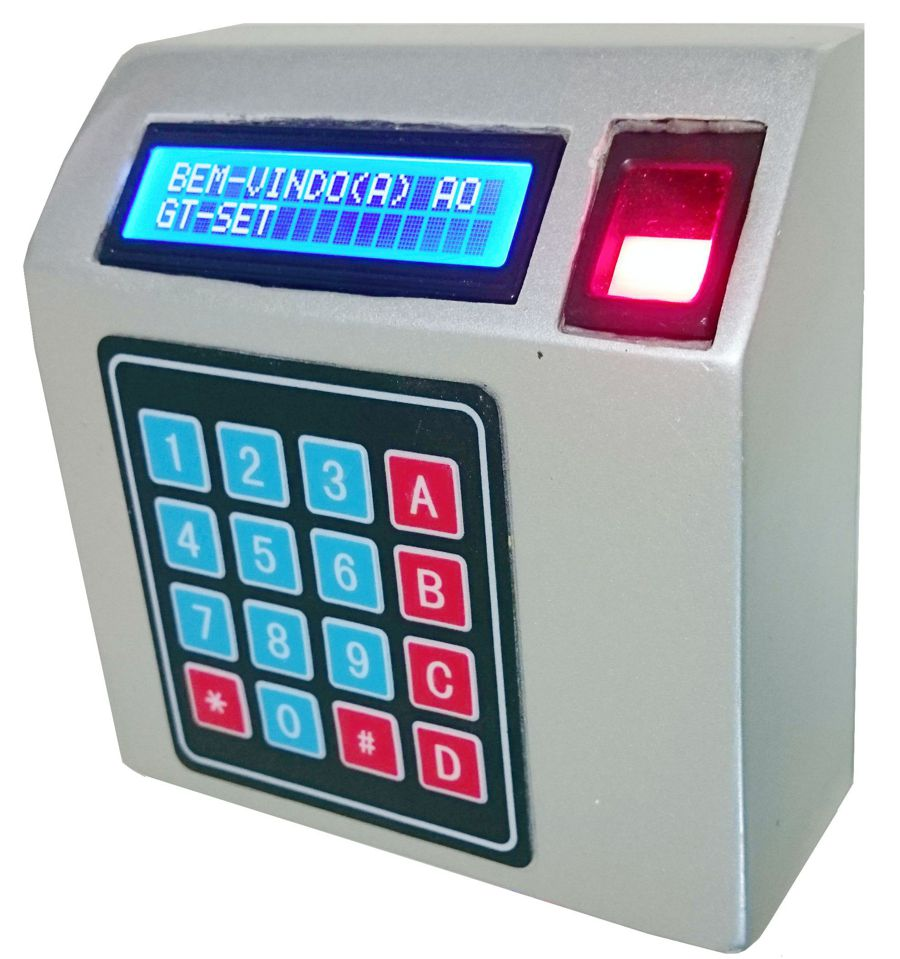
\includegraphics[scale=0.2]{figuras/cap4/setfinger_final.jpg}\\
  Fonte: Elaborada pelo autor.
  \label{setfinger_final}
  \end{center}
  \end{figure}





\section{\textit{Software} \label{software}}

Nesta seção serão abordados o banco de dados e os três módulos de \textit{software} que compõem o sistema Setfinger: cliente, servidor TCP e aplicação web. Entre o cliente e o servidor TCP há uma relação de dependência. Portanto, esses dois módulos serão apresentados em uma única seção para manter a organização do trabalho e simplificar a interpretação dos módulos  de \textit{software}. Por fim, será apresentada a aplicação de gerenciamento web.



\subsection{Cliente e servidor TCP}

O módulo de \textit{software} cliente é o \textit{software} embarcado na plataforma Arduino (MCU - Atmega 2560), escrito em linguagem C. Esse \textit{software} é responsável pela leitura da impressão digital do usuário, comunicação com o servidor TCP para verificar se tal usuário está cadastrado no banco de dados e qual seu nível de acesso, além de registrar o acesso desse usuário. O servidor TCP é uma aplicação do tipo server-side, desenvolvida com a plataforma node.js e escrita em linguagem javascript. Neste trabalho, essa aplicação possibilita a comunicação do cliente com o banco de dados que contém o cadastro e os registros de acesso dos usuários. Através dessa aplicação podem ser realizadas consultas e registros no banco de dados, de acordo com os comandos enviados pelo cliente. A lógica de funcionamento do aparelho Setfinger em conjunto com o servidor TCP pode ser melhor abstraída a partir do fluxograma mostrado na Figura~\ref{fluxograma_cliente-servidor}. Os principais blocos desse fluxograma são detalhados a seguir.

  
 \begin{figure}[!t]
 \begin{center}
  \caption{Fluxograma de funcionamento do aparelho Setfinger em conjunto com o servidor TCP - o fluxograma descreve as ações que envolvem o funcionamento do aparelho Setfinger em conjunto com o servidor TCP.}
  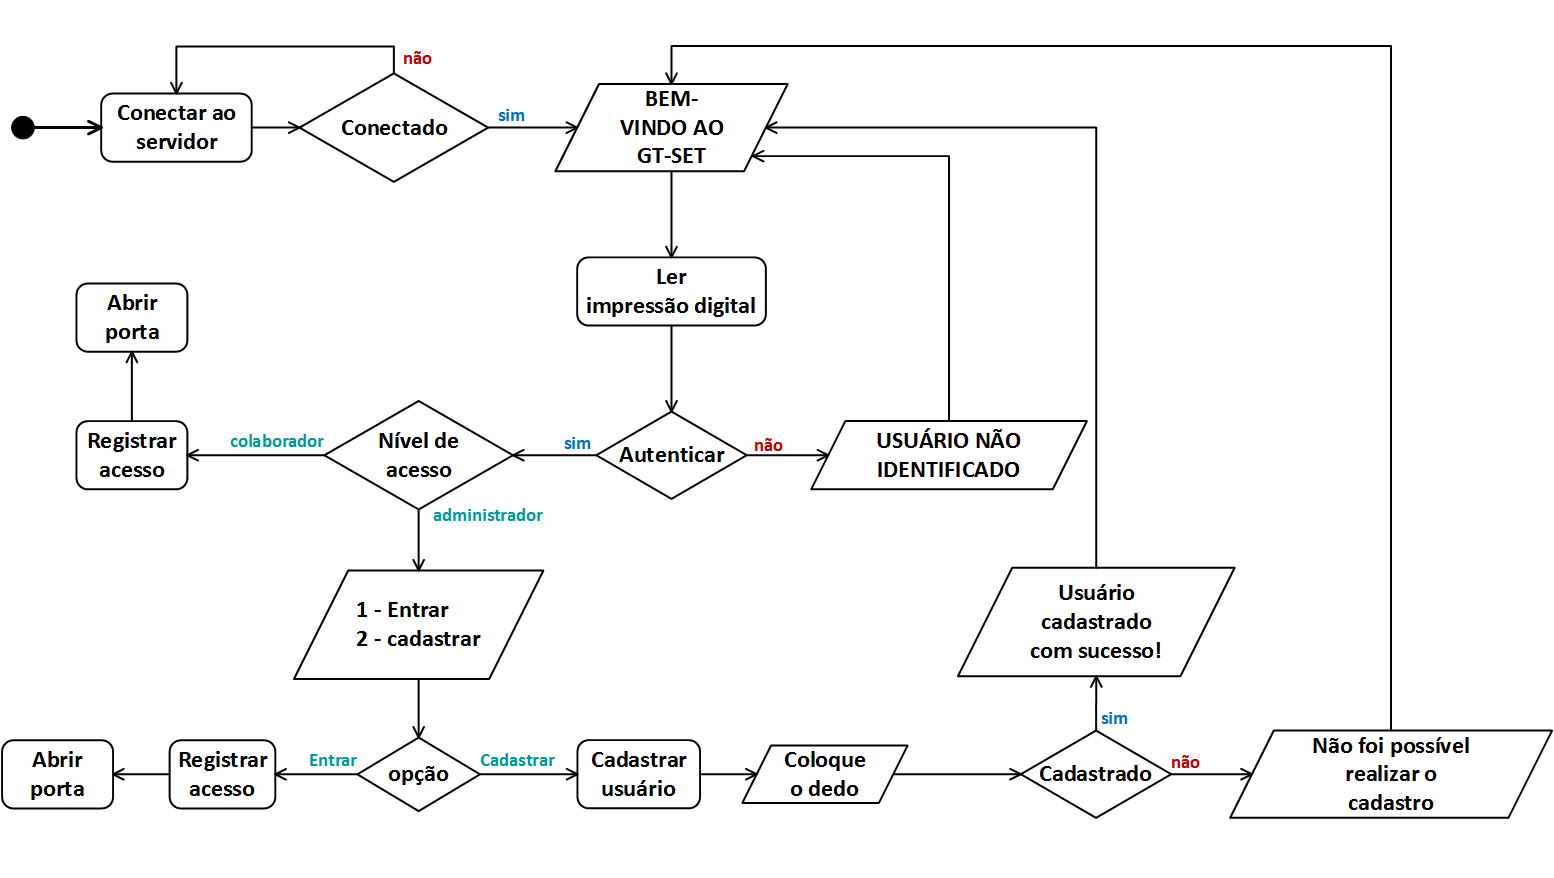
\includegraphics[scale=0.39]{figuras/cap4/fluxograma_cliente-servidor.png}\\
  Fonte: Elaborada pelo autor.
  \label{fluxograma_cliente-servidor}
  \end{center}
 \end{figure}
  
  \begin{itemize}
      \item Conectar ao servidor
      
      \begin{sloppypar}
      O cliente conecta-se ao servidor TCP através da execução da função \texttt{serverConnect()}, que faz parte do \textit{software} embarcado no Arduino (veja o Apêndice~\ref{apendice_conectar}). Essa função é responsável por estabelecer a conexão do cliente com o servidor TCP, através do método \texttt{client.connect(serverIP, serverPort)} nativo da biblioteca \textit{Ethernet.h}. Para estabelecer a conexão com o servidor TCP, o método \texttt{client.connect()} necessita receber o IP e a porta referentes ao servidor TCP. Essas configurações de IP e porta são definidas na declaração da biblioteca \texttt{Ethernet.h} (veja o Apêndice~\ref{apendice_ethernet}). Do lado do servidor é necessário utilizar o método \texttt{net.createServer()} para criar uma conexão do tipo TCP e atender as solicitações de conexão dos clientes (veja o Apêndice~\ref{apendice_createserver}).
      \end{sloppypar}
      
      Em qualquer ponto da execução do \textit{software} cliente, se a conexão for perdida por qualquer motivo, a execução volta para a conexão ao servidor.
      
      \item Ler impressão digital
      \begin{sloppypar}
      A função de leitura da impressão digital (\texttt{readFinger()}), implementada no \mbox{\textit{software}} cliente, realiza a captura da imagem da impressão digital e a comparação da impressão digital lida com as digitais cadastradas. As impressões digitais são armazenadas na memória \textit{flash} do sensor Fingerprint. A função que executa a leitura de impressões digitais no sensor Fingerprint é dividida em quatro eventos. \mbox{Esses} eventos são responsáveis por verificar se há um sensor conectado no sistema embarcado (\texttt{finger.verifyPassword()}), capturar a imagem da impressão digital (\texttt{finger.getImage()}), converter a imagem digital para um arquivo caracter (\texttt{finger.image2Tz()}) e buscar (\texttt{finger.fingerFastSearch()}) na memória do sensor, um arquivo carácter semelhante ao obtido na leitura da digital \cite{zfm-20}. Todos esses eventos (métodos) são nativos da biblioteca \texttt{Adafruit\_Fingerprint.h}. Desta forma, se a impressão digital lida for identificada, a função de leitura retornará um número do tipo inteiro que representa o ID associado a impressão digital identificada, caso contrário, a função deve retornar o valor $-1$.  
      \end{sloppypar}
      
      \item Autenticar
      
      Após a leitura da impressão digital, o ID retornado pela função \verb!readFinger()! é enviado para o servidor TCP no formato Notação de Objetos Javascript (\textit{Javascript Object Notation -- JSON})  \cite{bassett2015introduction, smith2015beginning}. O servidor TCP recebe o ID, consulta no banco de dados se há algum usuário com esse ID e responde ao cliente uma mensagem de erro, caso não haja nenhum usuário com tal ID, ou uma mensagem de confirmação com o nível de acesso do usuário autenticado. A digital do usuário deve estar cadastrada no sensor Fingerprint, porém a principal autenticação ocorre no servidor, pois o usuário pode estar cadastrado no sensor, mas se não estiver cadastrado no banco de dados, a sua autenticação não será confirmada. Isso facilita o gerenciamento online, tendo em vista que o gerenciamento remoto de usuários diretamente no sensor seria inviável.
      
      \nomenclature{JSON}{Notação de Objetos Javascript (\textit{Javascript Object Notation})}
      
      
      \item Nível de acesso
      
      Quando o ID informado no processo de autenticação pertencer a um usuário cadastrado no banco de dados, deve ser realizada uma consulta para verificar o nível de acesso desse usuário. Cada usuário possui um nível de acesso, o qual pode ser um colaborador (valor 0) ou um administrador (valor 1), de acordo com o diagrama de caso de uso mostrado na Figura~\ref{diagrama_autenticacao}. O nível de acesso de cada usuário será avaliado também na plataforma web.
      
      \begin{figure}[!t]
        \begin{center}
        \caption{Diagrama de caso de uso - autenticação do usuário no aparelho Setfinger.}
        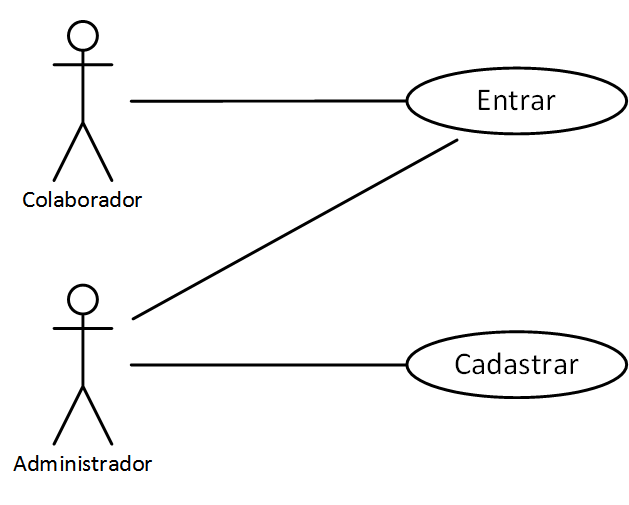
\includegraphics[scale=0.55]{figuras/cap4/diagrama_autenticacao.png}\\
        Fonte: Elaborada pelo autor.
        \label{diagrama_autenticacao}
        \end{center}
        \end{figure}
      
      \item Cadastrar usuário
      
      A operação de cadastro de usuário é dividida em duas etapas. A primeira etapa pode ser realizada somente através do aparelho Setfinger. Nessa etapa, é realizado o registro da impressão digital do usuário no sensor Setfinger. No ato do registro a impressão digital é gravada no sensor com um ID fornecido pelo servidor TCP, se a operação for realizada com sucesso o servidor TCP insere no banco de dados um novo usuário com o esse ID  e o nome ``NOVO USUÁRIO''. A memória flash do sensor Fingerprint tem um limite de $162$ impressões digitais \cite{zfm-20, zfm20ada}. Desta forma, quando a memória desse sensor estiver completamente ocupada, a reutilização de espaços de memória para registrar a impressão digital de novos usuário deve ser realizada somente quando o ID de uma impressão digital não pertencer a nenhum usuário cadastrado no banco de dados. Isto pode ocorrer quando um usuário for excluído do sistema. Portanto, o usuário pode estar cadastrado no sensor, mas se não estiver cadastrado no banco de dados, o espaço de memória ocupado pela sua digital poderá ser reutilizado. Logo, o controle de IDs é executado pelo servidor TCP e as informações referente as digitais disponíveis para o registro de novos usuários no sensor Fingerprint são mantidas no banco de dados, em uma tabela chamada \texttt{finger\_ids}.
      
      A segunda etapa de cadastro é possível somente após a ocorrência da primeira etapa. Nessa etapa, todos os usuários cadastrados como ``NOVO USUÁRIO'' devem permanecer na lista de Novos Usuário, até que o administrador do sistema atualize os dados de cada ``NOVO USUÁRIO'', através da plataforma web. 
      
      
      
      \item Registrar acesso
      
      Após a autenticação do usuário com nível de acesso ``colaborador'' ou após a escolha da opção ``Entrar'' por um usuário ``Administrador'', o aparelho Setfinger envia o ID do usuário para o servidor TCP, que insere no banco de dados o horário e a data de acesso desse usuário, em uma tabela chamada \verb!history!.
      
      \item Abrir porta
      
      A abertura da porta é a última operação a ser executada no processo de autenticação para acessar o ambiente controlado. No momento em que é autorizada a abertura da porta, um pino digital de saída ($5$ V) da MCU é setado em estado alto para acionar o relé associado ao fecho elétrico.
      
      \item Mensagens de display
      
      Durante a execução das operações previstas para o aparelho Setfinger, são exibidas mensagens em um display LCD para orientar o usuário na utilização do aparelho. A mensagem ``BEM-VINDO AO GT-SET'' é uma mensagem de boas vindas exibida sempre que o aparelho estiver no estado de leitura de impressão digital para autenticação, enquanto que as demais mensagens são exibidas de acordo com cada estado de operação do aparelho. Além disso, a mensagem de boas vindas ``BEM-VINDO AO GT-SET'' pode ser alterada diretamente no código do servidor TCP. Assim, no lugar de ``GT-SET'' pode ser colocado o nome do local em que o sistema Setfinger for instalado.
      
      
  \end{itemize}
  
  

\subsection{Plataforma web}

A plataforma web Setfinger possibilita o gerenciamento das informações mantidas no banco de dados. De acordo com o nível de acesso, essa plataforma classifica os usuários em duas categorias: os colaboradores e os administradores. Os colaboradores podem consultar somente seu próprio registro de acessos. Enquanto que os administradores do sistema podem atualizar o cadastro de usuários, consultar os acessos de usuários por data ou ID e gerar gráficos com base na frequência semanal ou mensal dos usuários. Na Figura~\ref{diagrama_autenticacao_web} são apresentados os casos de uso dos respectivos usuários. Esses casos de uso são discutidos nas Seções~\ref{sec:caso_uso:usuario} (colaboradores) e~\ref{sec:caso_uso:admin} (administrador).


\begin{figure}[!ht]
  \begin{center}
  \caption{Diagrama de caso de uso -- autenticação na plataforma web.}
  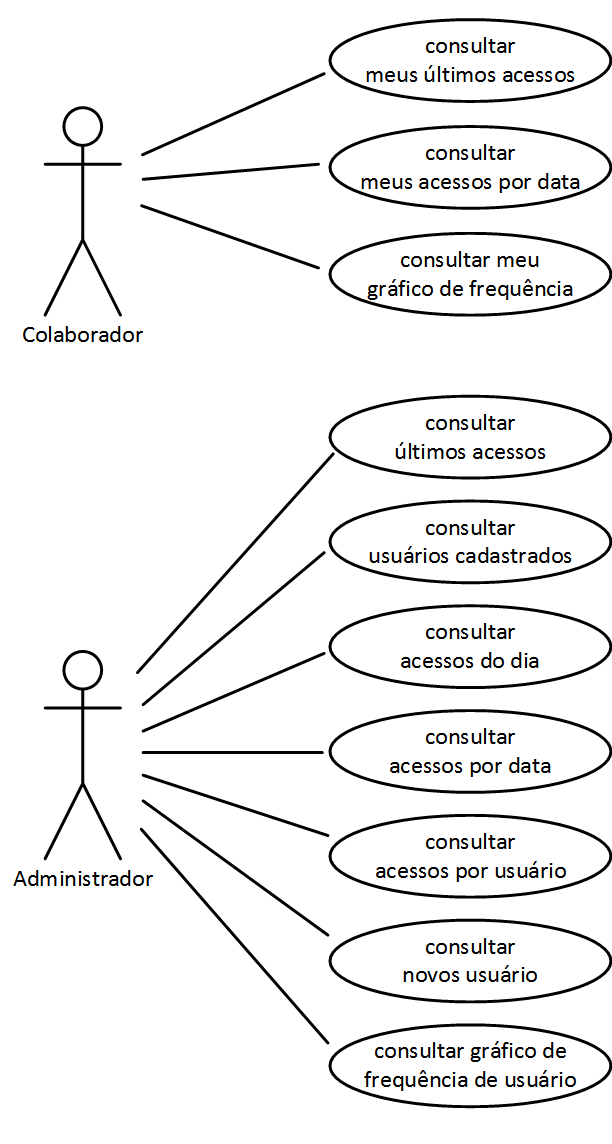
\includegraphics[scale=0.5]{figuras/cap4/diagrama_autenticacao_web.png}\\
  Fonte: Elaborada pelo autor.
  \label{diagrama_autenticacao_web}
  \end{center}
  \end{figure}
  
 Cada caso de uso apresentado no diagrama mostrado na Figura~\ref{diagrama_autenticacao_web} é uma página web. Essas páginas são divididas de acordo com as categorias de usuários. Portanto, as páginas de administrador são exclusivas ao acesso de administradores e as páginas de colaborador são exclusivas ao acesso de colaboradores. Além disso, essa plataforma possui uma tela de \textit{login} que antecede o acesso aos casos de uso. Esse \textit{login} é baseado em criptografia MD5 (\textit{Message-Digest algorithm 5}). Quanto a tecnologia, as páginas da plataforma proposta são responsivas, isto é, se redimensiona de acordo com o dispositivo que a executa (veja a Figura~\ref{setfinger_web}). Essa plataforma foi desenvolvida utilizando as linguagens HTML, CSS, PHP e Javascript e os \textit{frameworks} Bootstrap, Date picker bootstrap e Chart.js. A seguir, é apresentada uma descrição sucinta acerca de cada caso de uso.
 \nomenclature{MD5}{\textit{Message-Digest algorithm 5}}
  
\begin{figure}[!ht]
  \begin{center}
  \caption{Plataforma web Setfinger -- exemplo de uso em um dispositivo mobile.}
  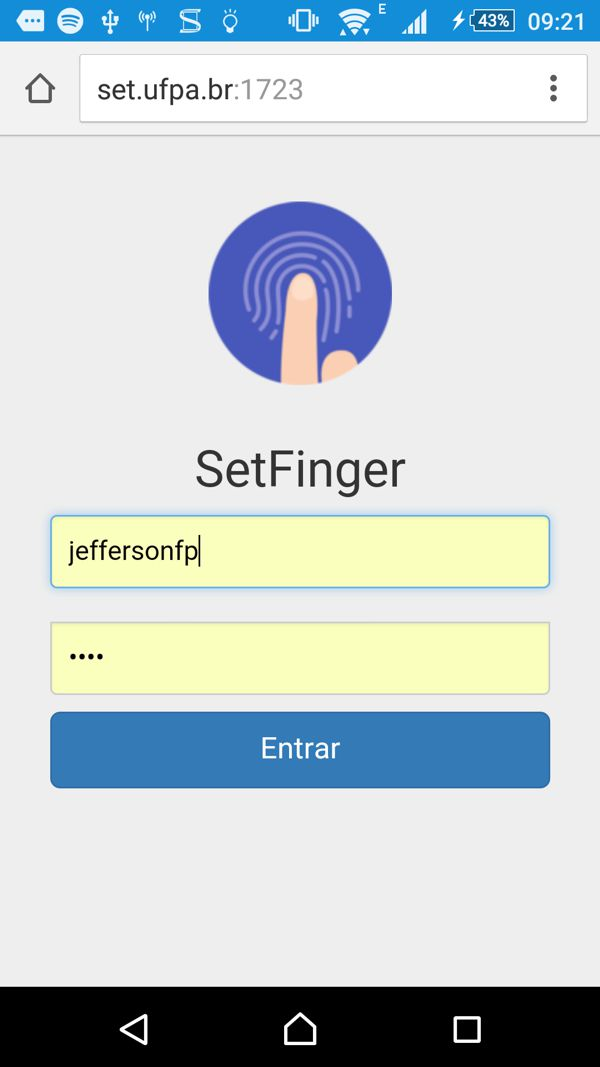
\includegraphics[scale=0.22]{figuras/cap4/setfinger_web.jpg}\\
  Fonte: Elaborada pelo autor.
  \label{setfinger_web}
  \end{center}
\end{figure}

  \subsubsection{Casos de uso dos colaboradores\label{sec:caso_uso:usuario}}
  \begin{itemize}
  
    \item Consultar últimos acessos
    
    Os últimos registros de acesso do colaborador são exibidos na página inicial da plataforma web, executada logo após o seu \textit{login}. Nessa página são exibidos os últimos 30 acessos registrados do colaborador.   
    
    \item Consultar meus acessos por data
    
    O colaborador pode consultar seus acessos por data. Desta forma, há um campo em que o usuário deve informar a data para a qual deseja consultar os seus registros de acessos.
    
    \item Consultar meu gráfico de frequência
  
    A partir dos registros de acesso do colaborador pode ser obtido o seu gráfico de frequência. Esse gráfico aponta a carga-horária mínima a ser cumprida e a carga-horária cumprida pelo colaborador dentro de um período que deve ser especificado no campo data (veja a Figura~\ref{web_frequencia_colaborador}).
  
    \begin{figure}[!ht]
    \begin{center}
    \caption{Plataforma web Setfinger - gráfico de frequência de usuário com nível de acesso \textit{colaborador}.}
     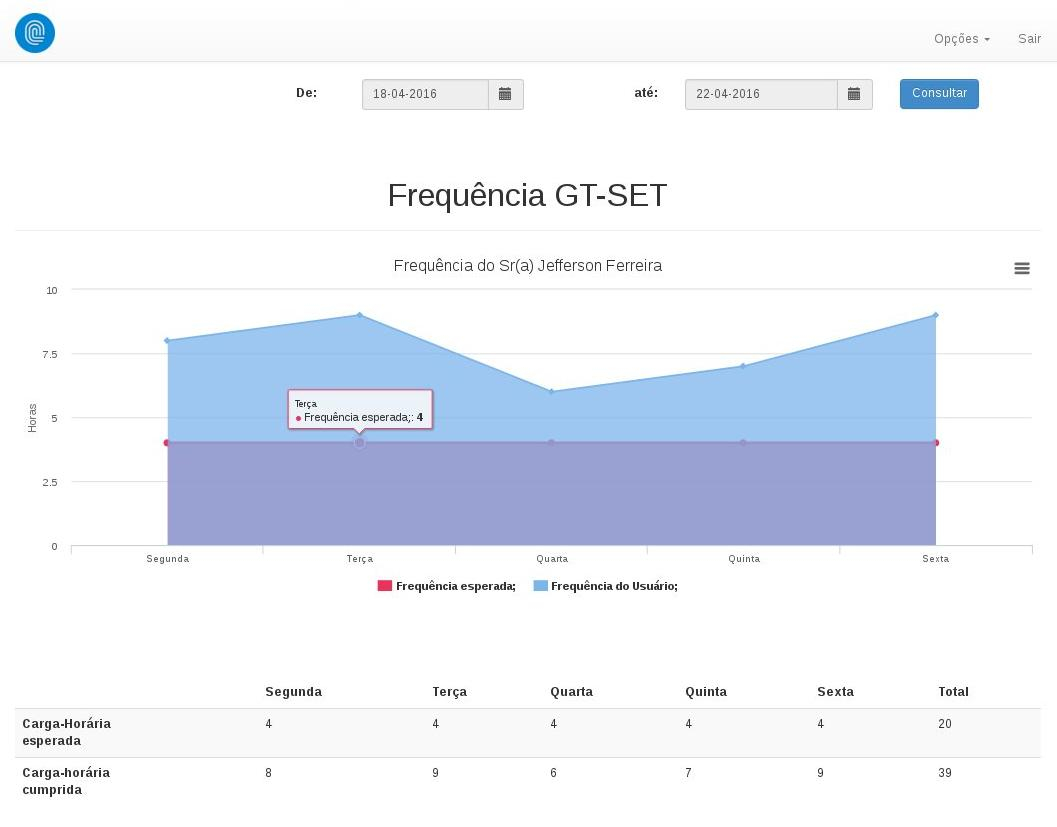
\includegraphics[scale=0.4]{figuras/cap4/web_frequencia_colaborador.jpg}\\
    Fonte: Elaborada pelo autor.
    \label{web_frequencia_colaborador}
    \end{center}
    \end{figure}
  
  
  
  \end{itemize}
  

  \subsubsection{Casos de uso dos administradores\label{sec:caso_uso:admin}}
  \begin{itemize}
  
    \item Consultar últimos acessos
    
    Na página inicial do administrador, executada após o seu \textit{login}, são exibidos os últimos 30 registros de acessos dos usuários cadastrados no sistema Setfinger.
    
    
    \item Consultar usuários cadastrados
    
    Usuários com nível de acesso \textit{administrador} podem consultar todos os usuários cadastrados no sistema. Nessa página são exibidos todos os usuários cadastrados no banco de dados, incluindo colaboradores e administradores, e seus dados.
    
    \item Consultar acessos do dia
    
    Os administradores podem consultar os registros de acessos ocorridos na data corrente.
    
    \item Consultar acessos por data
    
    Através dessa consulta são exibidos todos os registros de acessos ocorridos em uma data especificada pelo administrador.
    
    \item Consultar acessos por usuário
    
    Uma consulta pode ser realizada para verificar todos os registros de acessos de um usuário específico.
    
    \item Consultar novos usuários
    
    Todo usuário cadastrado no aparelho Setfinger é imediatamente cadastrado no banco de dados com o nome ``NOVO USUARIO'', permanecendo com o seu cadastro inativo até que seja realizada a atualização desse cadastro. Portanto, essa página exibe todos os usuários com atualização cadastral pendente.
    
    \item Consultar gráfico de frequência de usuário
  
    A partir dos registros de acessos de qualquer usuário, especificado ao sistema através do seu ID, pode ser gerado um gráfico de frequência. Esse gráfico aponta a carga-horária mínima a ser cumprida e a carga-horária efetiva cumprida pelo usuário dentro de um período, também especificado pelo administrador no campo data (veja a Figura~\ref{web_frequencia_admin}).
  
  
    \begin{figure}[!ht]
    \begin{center}
    \caption{Plataforma web Setfinger - gráfico de frequência de usuário com nível de acesso \textit{administrador}.}
     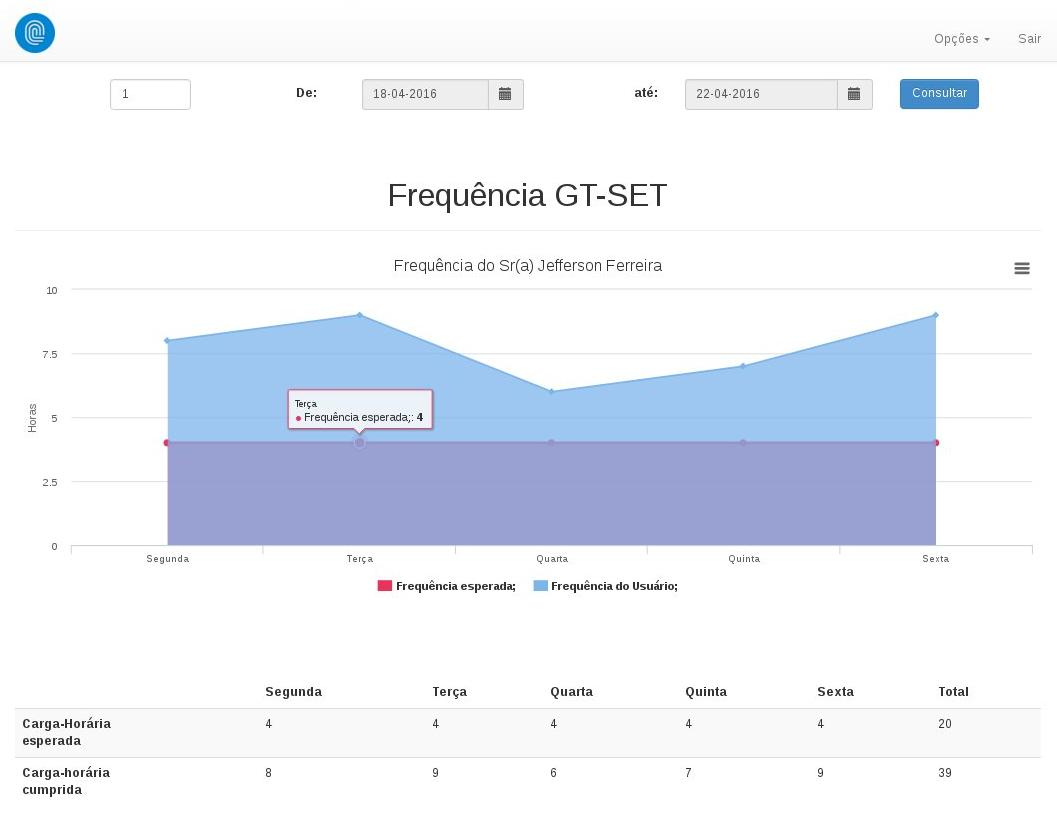
\includegraphics[scale=0.5]{figuras/cap4/web_frequencia_admin.jpg}\\
    Fonte: Elaborada pelo autor.
    \label{web_frequencia_admin}
    \end{center}
    \end{figure}
  
  
    
  \end{itemize}  
  
  
  
\subsection{Banco de dados}


A primeira etapa do projeto de um banco de dados é a construção de um modelo conceitual, através da modelagem conceitual. Um modelo conceitual é uma descrição abstrata do banco de dados, independente de implementação em um computador. O modelo conceitual registra os dados que devem aparecer no banco de dados, mas não registra como esses dados estão armazenados a nível de Sistema de Gerenciamento de Banco de Dados (\textit{Data Base Management System} -- DBMS). A técnica mais difundida de modelagem conceitual é a abordagem Modelo Entidade Relacionamento (\textit{Entity Relationship Model} -- ERM). Nessa técnica, um modelo conceitual é usualmente representado através de um diagrama, chamado Diagrama Entidade Relacionamento (\textit{Entity Relationship Diagram} -- ERD) \cite{heuser2009projeto}.

\nomenclature{DBMS}{Sistema de Gerenciamento de Banco de Dados (\textit{Data Base Management System})}
\nomenclature{ERM}{Modelo Entidade Relacionamento (\textit{Entity Relationship Model})}
\nomenclature{ERD}{(\textit{Entity Relationship Diagram})}


O uso de modelagem conceitual para projetar banco de dados pode auxiliar o DBMS a controlar a redundância de dados. A redundância de dados ocorre quando uma determinada informação está representada no sistema várias vezes, enquanto que a redundância controlada de dados acontece quando o \textit{software} tem conhecimento da múltipla representação da informação e garante a sincronia entre as diversas representações. Do ponto de vista do usuário externo ao sistema, tudo acontece como se existisse uma única representação da informação. Essa forma de redundância é utilizada para melhorar a performance global do sistema \cite{greenwald2007oracle, stephens2009sams}. Desta forma, são apresentados o modelo entidade-relacionamento e a modelagem do projeto de banco de dados do sistema Setfinger, nos diagramas mostrados na Figura~\ref{diagrama_DER} e Figura~\ref{diagrama_ER}, respectivamente.

\begin{sloppypar}
O diagrama mostrado na Figura~\ref{diagrama_ER} apresenta três tabelas: \texttt{finger\_ids}, \texttt{users} e \texttt{access}. 

A tabela \texttt{finger\_ids} é composta por 162 registros, cada registro contém um ID e o status de disponibilidade (\texttt{available}) desse ID, isto é, se o \texttt{available} de um ID for igual a $1$ significa que esse ID está disponível, caso seja igual a $0$ significa que está sendo utilizado por algum usuário. 

A tabela \texttt{users} contém os usuários cadastros. Portanto, cada registro contém os dados dos usuários, bem como, nome, \textit{login}, nível de acesso etc.

Por fim, a tabela \texttt{access} contém os registros de acesso dos usuários. Desta forma, cada registro contém a data e a hora de entrada do usuário no ambiente controlado.  



\end{sloppypar}

 \begin{figure}[!ht]
  \begin{center}
  \caption{Diagrama entidade-relacionamento - definição dos aspectos relacionais definidos para a modelagem do bando de dados do sistema Setfinger.}
  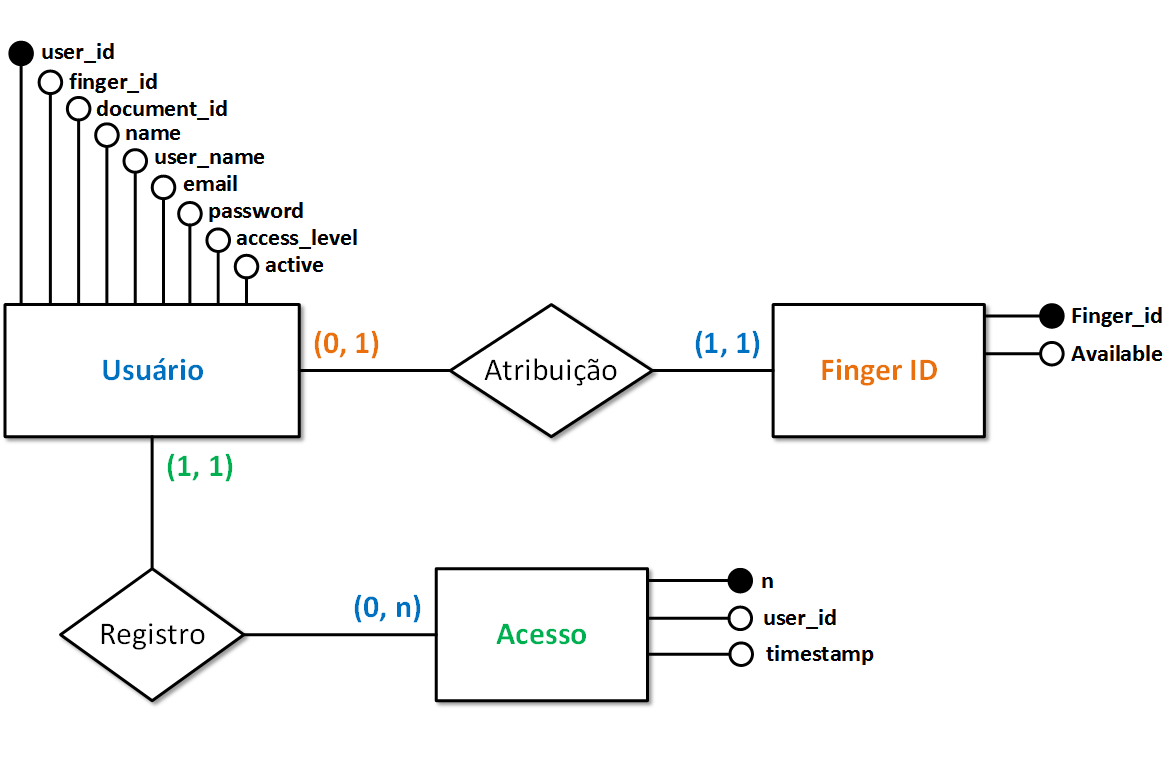
\includegraphics[scale=0.5]{figuras/cap4/diagrama_DER.png}\\
  Fonte: Elaborada pelo autor.
  \label{diagrama_DER}
  \end{center}
  \end{figure}
  
  
  
\begin{figure}[!ht]
  \begin{center}
  \caption{Diagrama de modelagem de banco de dados relacional - os relacionamentos entre as entidades do banco de dados do sistema Setfinger são definidos a partir do DBMS Phpmyadmin.}  
  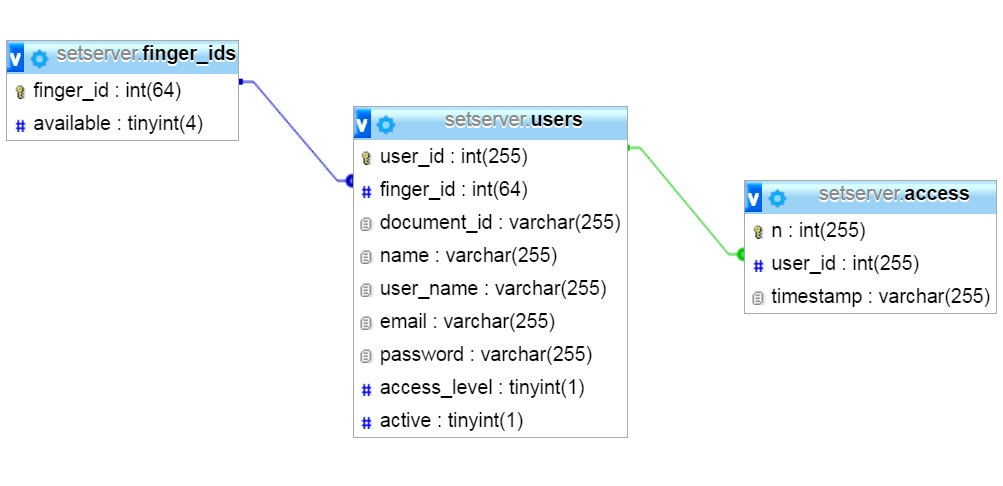
\includegraphics[scale=0.55]{figuras/cap4/diagrama_ER.jpg}\\
  Fonte: Elaborada pelo autor.
  \label{diagrama_ER}
  \end{center}
  \end{figure}
  

  

\section{Considerações}

Com relação ao desenvolvimento do módulo de \textit{hardware} houveram algumas dificuldades quanto a documentação de alguns dispositivos, como o sensor Fingerprint que possui \textit{datasheet} em inglês, porém pouco detalhada. Esse componente, assim como o display LCD, é de fabricação chinesa. Portanto, a documentação detalhada desses componentes estão disponíveis na língua Mandarin. O material empregado na confecção do aparelho Setfinger proposto na Seção~\ref{hardware_setfingerproposto}, custou R{\$} 404,55 (quatro centos e quatro reais e cinquenta e cinco centavos). A aquisição de grande parte desse material, tal como cabos com dimensão e número de conexões específicas, gabinetes para embutir o aparato eletrônico, CI's e outros componentes eletrônicos, foi difícil devido a baixa oferta desse tipo de produtos em Belém-Pa. Desta forma, houve a necessidade de encomenda de alguns componentes e adaptações utilizando materiais alternativos, para chegar o mais próximo possível do resultado desejado. Além disso, todos os diagramas e fluxogramas apresentados neste capítulo foram desenvolvidos no \textit{software} Microsoft Visio, com base na aplicação de Linguagem Unificada de Modelagem (\textit{Unified Modeling Language} -- UML) \cite{biafore2007visio, naiburg2001uml}. Exceto o diagrama de modelagem de banco de dados mostrado na Figura~\ref{diagrama_ER}, que foi elaborado do DBMS Phpmyadmin.

\nomenclature{UML}{Linguagem Unificada de Modelagem (\textit{Unified Modeling Language})}

Os códigos do sistema Setfinger estão disponíveis em \href{https://github.com/jeffersonfpalheta/setfinger_system}{\textit{github.com/jeffersonfpalheta}}.


\chapter{Testes e Resultados\label{cap:resultados}}
 Neste Capítulo são relatados os testes realizados sobre o aparelho Setfinger e o módulo servidor. Os objetivos dos testes de \textit{hardware} são: avaliar o desempenho da MCU e do Controlador Ethernet; verificar a eficiência do circuito de alimentação; verificar as conexões via cabos e trilhas para identificar e corrigir possíveis falhas elétricas; e confirmar o funcionamento de cada componente através destes unitários. Os objetivos dos testes de \textit{software} são: avaliar a comunicação do servidor TCP com o aparelho Setfinger, avaliar o desempenho do banco de dados Mysql, verificar a compatibilidade dos \textit{frameworks}, utilizados no módulo servidor, com diferentes sistemas operacionais, e validar as funcionalidades da página de gerenciamento e verificar o conteúdo do banco de dados.
 
 
 
\section{Aparelho Setfinger\label{testes&resultados_aparelho}}

Além do \textit{hardware} proposto, o sistema Setfinger foi testado em conjunto com as versões de \textit{hardware} 1.0 e 2.0 apresentadas no Apêndice~\ref{hardware_1.0} e~\ref{hardware_2.0}, respectivamente. Todas essas versões foram instaladas e testadas no CTIC, e permanecem sendo utilizadas para o propósito ao qual foram destinadas. Desta forma, são apresentados a seguir os testes realizados sobre o \textit{hardware} Setfinger e os seus respectivos resultados.


\begin{itemize}
    \item O aparelho Setfinger foi mantido ligado durante um período de no mínimo 30 dias, 24 horas por dia, e não apresentou problemas com o uso contínuo.
    
    \item Foi realizado teste unitário para verificar a precisão de leitura das teclas do \textit{keypad} com o circuito \textit{one wire kaypad}. Além disso, foi realizado um teste de desgaste das teclas, no qual verificou-se o funcionamento das teclas após serem pressionadas cerca de 100 vezes. O circuito \textit{one wire kaypad} utilizado para a redução de fios de conexão com o Arduino não apresentou o resultado esperado, pois ocorreram erros na leitura das teclas pressionadas. Além disso, notou-se que a leitura correta das respectivas teclas do dispositivo \textit{keypad} ocorre somente quando esse dispositivo é alimentado na saída $5$ V fornecido pelo Arduino. Quando, alimentado na saída $5$ V fornecido pelo regulador extra L7805, as teclas pressionadas são atribuídas a caracteres não correspondentes aos quais elas representam. Por exemplo, quando a tecla ``1'' é pressionada, o aparelho Setfinger a reconhece como a tecla ``2''. Portanto, propõe-se a substituição do circuito \textit{one wire kaypad} por uma nova abordagem utilizando o circuito integrado expansor de portas PCF8574AP Philips/NXP \cite{pcf8574}, baseado em tecnologia I2C. Esse Circuito Integrado (CI) possibilita a redução do numero de conexões do teclado ao Arduino, pois necessita apenas de duas vias de dados (SDA e SCL) e duas vias de alimentação ($5$ V e GND).

    \nomenclature{CI}{Circuito Integrado}
    
    
    \item Foram gravadas apenas as impressões digitais de 15 usuários no leitor Fingerprint, devido a falta de voluntários. O fabricante do sensor Fingerprint informa em sua documentação que a memória \textit{flash} desse dispositivo tem capacidade para o armazenamento de apenas 162 modelos de impressões digitais (\textit{templates}) \cite{zfm-20, zfm20ada}. No entanto, foi realizado um teste, no qual as impressões digitais de um mesmo usuário foram gravadas além de 162 vezes. Desta forma, para cada gravação foi atribuído um ID sequencialmente, de 1 a 200. O \textit{datasheet} do sensor Fingerprint ZFM-20 não fornece informações que possibilitem a compreensão lógica de gravação dos modelos de impressão digital. Além disso, a quantidade de usuários cadastrados nesse teste é insuficiente para verificar o comportamento do sensor mediante a gravação do número limite de impressões digitais recomendado pelo fabricante. Os processos internos de gravação e leitura do sensor Fingerprint não são objetos de estudo deste trabalho. Portanto, não foi possível concluir o que ocorre após a gravação de 162 modelos digitais. Empiricamente, as possibilidades são que o sensor sobrescreva aleatoriamente algum espaço de memória ocupado por um modelo digital ou que ele possua um espaço de memória suficiente para gravar um número maior que 162 \textit{templates}. 
    
    Quanto aos resultados de sua utilização, o sensor Fingerprint apresentou um bom desempenho no reconhecimento das impressões digitais dos usuários. No entanto, a gravação da digital dos usuários deve ser realizada de forma adequada, caso contrário o sensor apresenta dificuldades para o reconhecimento da impressão digital do usuário. Desta forma, no momento da gravação da impressão digital, preferencialmente com o dedo limpo, o usuário deve manter o seu dedo corretamente pressionado contra a lente óptica do sensor no momento da captura da imagem da sua impressão digital.
    
    \item Foi realizada uma verificação de temperatura sobre os reguladores L7805, L7809 e AMS 1117, a fim de detectar a ocorrência de possíveis sobreaquecimentos que podem danificar os componentes do \textit{hardware} Setfinger. Através desse teste observou-se um aquecimento razoável sobre os reguladores citados. No entanto, não houve sobreaquecimento e nenhuma ocorrência de defeitos eletrônicos devido a excessos de temperatura.
     
\end{itemize}



\section{Módulo Servidor (Setsever)\label{testes&resultados_servidor}}

A seguir são apresentados os testes realizados sobre o servidor TCP, banco de dados e plataforma web, e os resultados obtidos a partir da aplicação desses testes. 


\begin{itemize}
    
  \item O banco de dados e a plataforma web dependem de um servidor web. Desta forma, foram instalados os servidores web LEMP (Linux Nginx MySQL PHP) e WAMP (Windows Apache Mysql PHP), nos sistemas operacionais Linux e Windows, respectivamente. No Windows Seven foi instalado e utilizado a plataforma de desenvolvimento web WAMP. No Linux o servidor Setserver foi testado em duas distribuições diferentes, Debian 8 e Mint 17. Em ambas as versões foi utilizado a plataforma LEMP. O servidor web WAMP foi facilmente utilizado, não apresentando erros durante o processo de instalação, tampouco durante a execução dos seus serviços. No Mint 17 a instalação foi realizada com sucesso, sem a ocorrência de erros. No entanto, no Debian 8 houve uma grande dificuldade na instalação do \textit{Phpmyadmin}. 
  \nomenclature{WAMP}{Windows Apache Mysql PHP}
  \nomenclature{LEMP}{Linux Nginx MySQL PHP}
  
  \item O Servidor TCP é baseado em node.js, por isso depende da plataforma node.js, a qual possui versões para ambos os sistemas operacionais supracitados. Portanto, o node.js foi instalado nos sistemas operacionais Windows Seven, Debian 8 e Mint 17, para a execução do \textit{software} servidor TCP. Além disso, os comandos utilizados em interpretadores de linha de comandos, para a execução de \textit{software} baseados em node.js ocorre de maneira semelhante em todas as suas versões. O \textit{software} servidor TCP funcionou normalmente em todos os sistemas operacionais em que o node.js foi instalado, apresentando comportamento semelhante em todos os testes realizados.  
  
  \item A plataforma web foi hospedada nos servidores web LEMP e WAMP. No WAMP a plataforma web Setfinger foi testada apenas no \textit{localhost}. No entanto, no LEMP a plataforma web foi testada com um domínio público. Através da plataforma web foram cadastrados 15 usuários e registrados mais de 1000 acessos de usuários. Além disso, o banco de dados Mysql apresentou um bom desempenho e as consultas e inserções realizados pelo servidor TCP e pela plataforma web, funcionaram normalmente.   
  
  


\end{itemize}



\chapter{Conclusão\label{cap:conclusao}}

Neste trabalho foi apresentada uma solução de controle de acesso biométrico autenticado por impressão digital, na qual o projeto foi elaborado visando a utilização de recursos de \textit{hardware} e \textit{software} livre. Esse sistema conta com um aparelho biométrico de interface com o usuário e um módulo servidor.

O \textit{hardware} proposto, denominado aparelho Setfinger, trata-se de um aparelho biométrico baseado na plataforma Arduino. Além do \textit{hardware} proposto, foram produzidas outras duas versões de \textit{hardware} (1.0 e 2.0). Portanto, o \textit{hardware} proposto é a terceira versão de uma série de três versões produzidas ao longo da execução do projeto Setfinger, sendo a terceira versão o resultado da melhoria das versões anteriores. O Setfinger é um aparelho biométrico que disponibiliza a leitura, gravação e identificação de impressões digitais. Além disso, todas as versões desse aparelho foram instaladas, testadas e permanecem em funcionamento no CTIC.

O módulo servidor, denominado servidor Setserver, é composto por uma servidor TCP baseado em node.js, um banco de dados Mysql e uma plataforma web de gerenciamento online. O servidor TCP é responsável por estabelecer a comunicação e trocar informações com o aparelho Setfinger, além de gravar no banco de dados os registros de acessos e os cadastros dos usuários. Enquanto que a plataforma web é a interface de gerenciamento de dados que possibilita aos administradores do sistema consultarem os registros de acesso de todos os usuários por data ou ID, verificar os usuários cadastrados e gerar gráficos de frequência com a relação dias/horas. 

Com relação aos desafios enfrentados ao longo do desenvolvimento desse sistema, a confecção dos protótipos eletrônicos foi um processo que se tornou complexo devido as dificuldades de aquisição de componentes compatíveis com as necessidades do projeto, como cabos com dimensão e número de conexões específicas, gabinetes para embutir o aparato eletrônico, CI's e outros materiais eletrônicos. Desta forma, houve a necessidade de adaptações utilizando materiais alternativos, para chegar o mais próximo possível do resultado desejado. Portanto, de acordo com as conclusões obtidas, na Seção~\ref{cap:trabalhos_futuros} são apresentadas algumas sugestões de trabalhos futuros para aperfeiçoar o sistema proposto e aumentar sua escalabilidade.



\section{Trabalhos futuros\label{cap:trabalhos_futuros}}


Nesta seção são apresentadas algumas propostas de trabalhos futuros de acordo com as necessidades de aperfeiçoamento e escalabilidade observadas a partir dos resultado apresentados pelo sistema proposto neste trabalho. As propostas de trabalhos futuros são:

\begin{itemize}
    
    \item Adequar o sistema proposto as normas estabelecidas pelo Ministério do Trabalho e Emprego (MTE), de acordo com a portaria que regulamenta o Sistema de Registro Eletrônico de Ponto (SREP): Portaria Nº 1.510, de 21 de Agosto de 2009, publicada no Diário Oficial da União (DOU) de 25/08/2009, a fim de tornar o sistema Setfinger compatível com os sistemas de Planejamento de Recurso Corporativo (\textit{Enterprise Resource Planning} -- ERP).
    
    \nomenclature{MTE}{Ministério do Trabalho e Emprego}
    \nomenclature{DOU}{Diário Oficial da União}
    \nomenclature{ERP}{Planejamento de Recurso Corporativo (\textit{Enterprise Resource Planning})}
    \nomenclature{SREP}{Sistema de Registro Eletrônico de Ponto}
    
    \item Desenvolver a integração do sistema Setfinger com o Sistema Integrado de Gestão de Atividades Acadêmicas (SIGAA), da Universidade Federal do Pará.
    
    \nomenclature{SIGAA}{Sistema Integrado de Gestão de Atividades Acadêmicas}
    
    \item Confeccionar uma placa única com microcontrolador Atmega 2560 e Wiznet W5100 integrados, eliminando assim o Arduino e o Ethernet Shield. Além disso, produzir um gabinete em impressora 3D ou em material acrílico, para embutir o \textit{hardware} do aparelho Setfinger. 
    
    \item Elaborar uma versão de aparelho Setfinger baseado em Raspberry PI com leitor biométrico U.are.U 5000, com o intuito de oferecer uma versão de aparelho \textit{offline} independente de um servidor.
    
    \item Implementar métodos de segurança criptográfica na comunicação cliente-servidor.

    \item Migrar a plataforma web Setfinger para Javascript e o banco de dados Mysql para Mongo DB. Desta forma, não haverá a necessidade de um servidor web, como WAMP ou LEMP, pois o serviço web realizado por esses servidores pode ser executado pelo node.js. Consequentemente, o processamento da plataforma será realizado do lado do cliente.


\end{itemize}
%Apêndices
\renewcommand\appendixname{Apêndice}
\appendix
\addcontentsline{toc}{chapter}{Apêndices}




\chapter{Função \textit{serverConnect()} \label{apendice_conectar}}

A função \textit{serverConnect()} faz parte do \textit{software} cliente e é responsável por conectar o aparelho Setfinger (cliente) ao servidor TCP.

\begin{lstlisting}
void serverConnect() {  
  client.stop();
  AuthOk = false;
  Serial.println("Connecting...");
  printMessage("CONECTANDO...","");

  if(client.connect(serverIP, serverPort)) {
    Serial.println("Connected!");

    StaticJsonBuffer<64> jsonBuffer;                    
    JsonObject& root = jsonBuffer.createObject();
    root["type"] = "conn";
    root["hwid"] = SETFINGER_HWID;
    char buffer[64];
    root.printTo(buffer, sizeof(buffer)); 
    client.print(buffer);
    
    fullCircle = false;
    waitingResponse = false;
    waitingKeypress = false;
  } else {
    printMessage("ERRO", "ID: #0001");
    Serial.println("Connection failed!");
    redColorAlert();
  }
}
\end{lstlisting}



\chapter{Declaração das bibliotecas Ethernet.h e SPI.h \label{apendice_ethernet}}
O presente trecho de código faz parte do módulo de \textit{software} cliente, e é responsável pela inclusão das bibliotecas necessárias para o funcionamento do controlador ethernet. Nesse código são definidas as configurações de porta e IP do servidor ao qual o cliente deve se conectar.

\begin{lstlisting}
#include <SPI.h> 
#include <Ethernet.h>
byte mac[] = { 0xDE, 0xAD, 0xBE, 0xEF, 0xFE, 0xED };
IPAddress serverIP(192,168,14,103); 
const int serverPort=7000; //source port (1-65535)

EthernetClient client;
\end{lstlisting}



\chapter{Método \textit{createServer()} \label{apendice_createserver}}
O método \textit{createServer()} faz parte do \textit{software} servidor TCP e é responsável por criar uma conexão do tipo TCP.

\begin{lstlisting}
var fingerServer = net.createServer(setServer)
    .listen(config.port, () => log('server', 
    "O servidor esta sendo iniciado..."))
    
    .on('connection', (data) => log('TCP', 
    'Conexao estabelecida de ' +
    chalk.underline(data.remoteAddress + ':' + data.remotePort)))
    
    .on('listening', (data) => log('server', 
    'O servidor foi iniciado em ' + 
    chalk.underline(fingerServer.address().address + ':
    ' + fingerServer.address().port)))
    
    .on('error', (err) => errorHandler(err));
\end{lstlisting}








\chapter{Versão de \textit{hardware} Setfinger 1.0\label{hardware_1.0}}



A primeira versão de \textit{hardware} foi montada em um único módulo, inicialmente embutida em uma carcaça confeccionada em Placa de Fibra de Média Densidade (\textit{Medium Density Fiberboard} -- MDF) e alumínio (veja a Figura~\ref{setfinger_v1_1}).
Posteriormente, o aparato eletrônico foi embutido em um gabinete plástico (veja Figura~\ref{setfinger_v1_2}), e instalado ao lado da porta da sala do GT-SET. As características gerais desse aparelho são apresentadas a seguir:
\nomenclature{MDF}{Placa de Fibra de Média Densidade (\textit{Medium Density Fiberboard})}


\begin{itemize}

\item Alimentação

O Arduino e os componentes conectados à ele, são alimentados por uma fonte de \mbox{$5$ V/$1$ A}. A fechadura eletrônica é alimentada por uma fonte de \mbox{$12$ V/$1.5$ A}.

\item Fechadura eletrônica

O aparelho Setfinger é integrado a um fecho eletromagnético de $12$ V/500 mA. O fecho é conectado a um circuito, mostrado na Figura~\ref{circuito_fecho},
que contém um relé. Esse relé é controlado pelo aparelho Setfinger. Desta forma, o fecho é acionado para liberar a abertura de uma porta, quando o relé recebe um sinal elétrico de $5$ V do módulo de \textit{hardware}. Além disso, o circuito, no qual o fecho é conectado, é responsável pela proteção elétrica do fecho e da fonte de alimentação, controlando sobretensões, a fim de evitar danos nesses dispositivos.

\item Setshield

O setshield, mostrado na Figura~\ref{setshield_v1}, é uma PCB que conecta ao Arduino os seguintes dispositivos: display LCD, teclado matricial, sensor fingerprint, buzzer, led e relé. A maioria das conexões entre esses dispositivos e placa Setshield, foram feitas por meio de cabos soldados à PCB. Esse tipo de integração, empregando Shields, é comum em aplicações com Arduino \cite{isikdag2015enhanced, grimmett2014arduino, premeaux2012arduino}.

\item Conexão com o Arduino Mega

Ao Arduino Mega foi acoplado um \textit{Ethernet Shield}, para comunicação do sistema embarcado com o servidor, e o Setshield foi acoplado ao \textit{Ethernet Shield}. A placa \textit{Ethernet Shield} apresenta o formato de um Arduino Uno, porém o Arduino Mega apresenta um \textit{layout} de placa maior que o \textit{layout} do modelo Uno. Portanto, ao ser conectada ao Arduino Mega, o \textit{Ethernet Shield} não tem contato com todos os pinos desse modelo de Arduino. Desta forma, foi soldado um cabo na placa Setshield, que é conectado  ao Arduino Mega, pois, devido a distância entre as placas não foi possível utilizar barra de pinos.
    
\end{itemize}




\begin{figure}[!t]
  \begin{center}
  \caption{Primeira versão de carcaça para o \textit{hardware} (SetFinger 1.0) - todo o aparato eletrônico é embutido em uma carcaça confeccionada em material \textit{mdf} e alumínio.}
  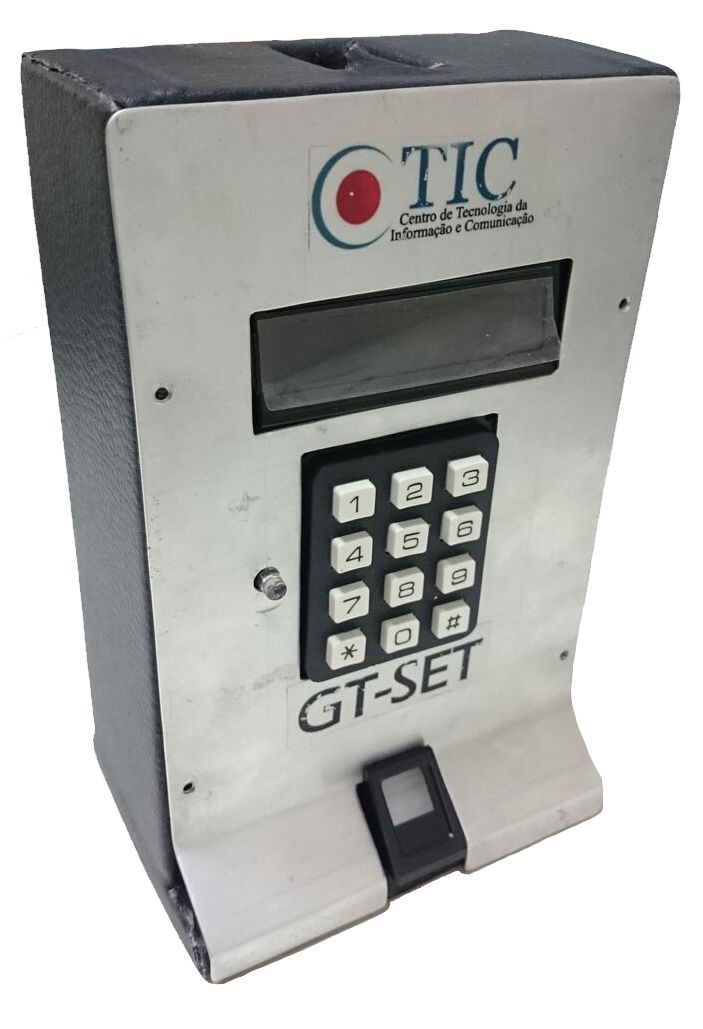
\includegraphics[scale=0.8]{figuras/cap4/setfinger_v1_1.jpg}\\
  Fonte: Elaborada pelo autor.
  \label{setfinger_v1_1}
  \end{center}
  \end{figure}
  
  
\begin{figure}[!t]
  \begin{center}
  \caption{Primeira versão de \textit{hardware} (SetFinger 1.0) - aparato eletrônico embutido em gabinete plástico}
  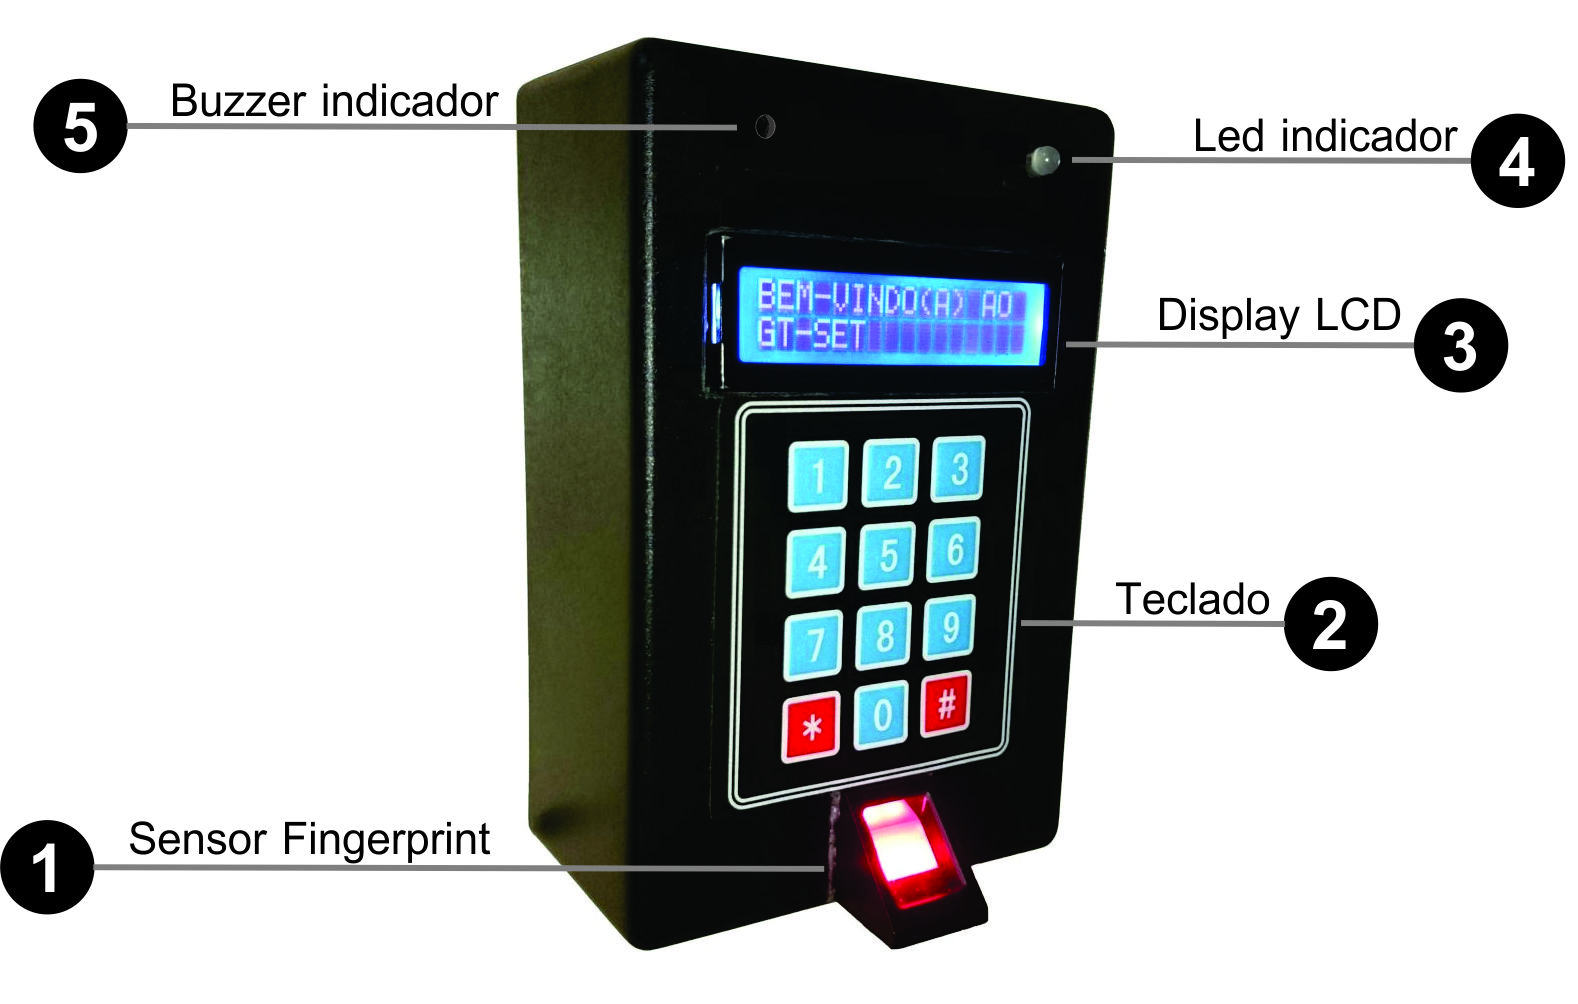
\includegraphics[scale=0.7]{figuras/cap4/setfinger_v1_2.jpg}\\
  Fonte: Elaborada pelo autor.
  \label{setfinger_v1_2}
  \end{center}
  \end{figure}


\begin{figure}[!t]
  \begin{center}
  \caption{Circuito de controle e proteção do fecho elétrico da versão de \textit{hardware} 1.0. Esse módulo de \textit{hardware} foi produzido somente na versão de aparelho Setfinger 1.0, nas demais versões o módulo de controle do fecho elétrico foi projetado na placa Setshield.}
  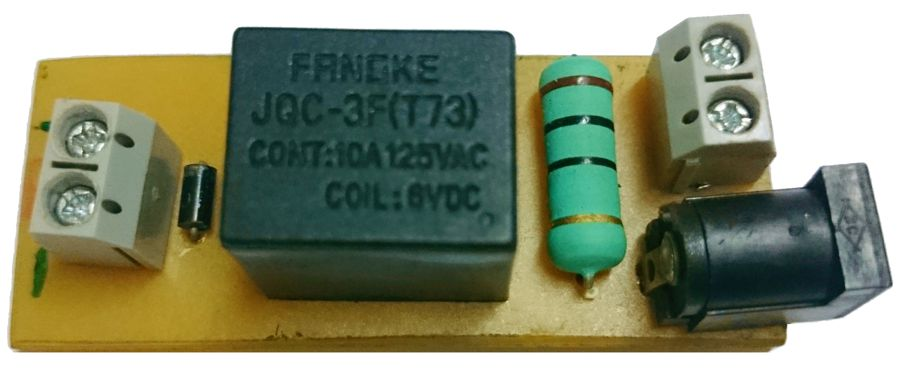
\includegraphics[scale=0.25]{figuras/cap4/circuito_fecho.jpg}\\
  Fonte: Elaborada pelo autor.
  \label{circuito_fecho}
  \end{center}
  \end{figure}
  

\begin{figure}[!t]
  \begin{center}
  \caption{Placa Setshield 1.0}
  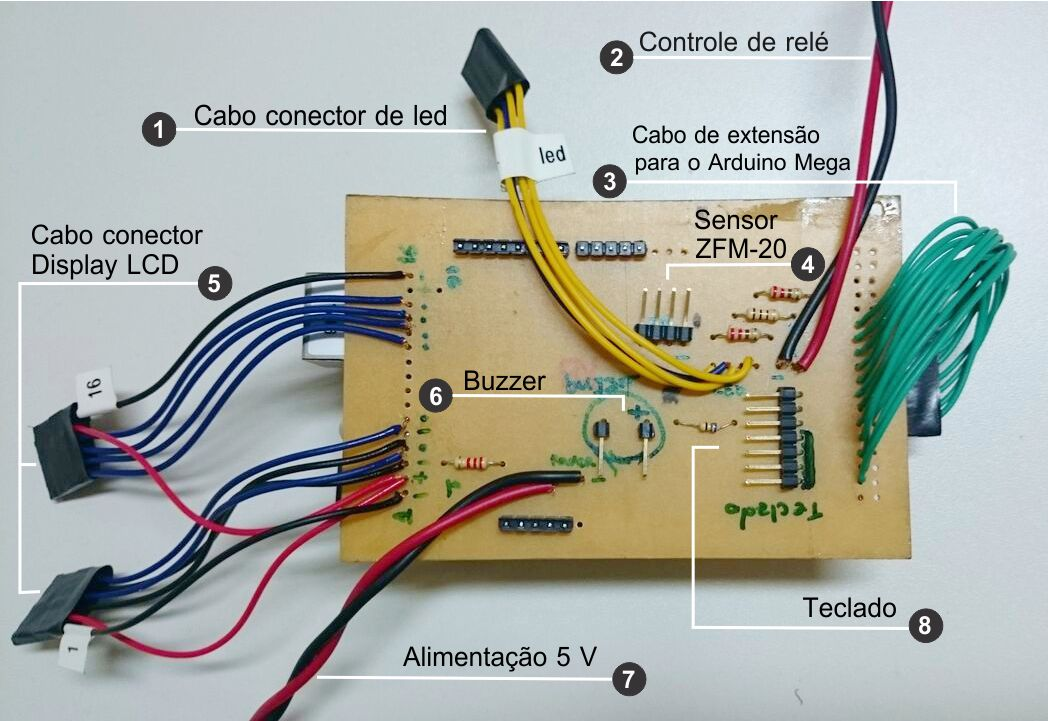
\includegraphics[scale=0.5]{figuras/cap4/setshield_v1.jpg}\\
  Fonte: Elaborada pelo autor.
  \label{setshield_v1}
  \end{center}
  \end{figure}




\chapter{Versão de \textit{hardware} Setfinger 2.0\label{hardware_2.0}}


Na segunda versão de \textit{hardware}, o aparelho Setfinger é dividido em dois módulos, por questões de segurança. Esses módulos são: um módulo interno à sala e um módulo externo,  (veja as Figuras~\ref{setfinger_v2} e ~\ref{setfinger_v2_p2}, respectivamente). Desta forma, o usuário só tem contato com o módulo externo, o qual é composto pelos seguintes componentes: teclado matricial, sensor fingerprint e Display LCD.  O módulo interno é composto pelo Arduino Mega, \textit{Ethernet Shield} e Setshield. As características gerais desse aparelho são apresentadas a seguir:


\begin{itemize}

\item Alimentação

O Arduino e os componentes conectados à ele, são alimentados pela mesma fonte utilizada para acionar a fechadura eletrônica, uma fonte chaveada de $12$ V/$5$ A. Para isso, foi utilizado um regulador de 5V, modelo 708S05, a fim de eliminar a fonte de $5$ V utilizada na versão 1.0 para alimentar o Arduino. 

\item Fechadura eletrônica

O aparelho Setfinger é integrado a um fecho eletromagnético de $12$ V/200 mA. 


O fecho é conectado diretamente ao módulo de \textit{hardware} interno, que contém um relé acoplado à placa Setshield. Desta forma, o fecho é acionado para liberar a abertura da porta, quando o relé é acionado com um sinal elétrico de $5$ V. 

\item Setshield

O setshield, mostrado na Figura~\ref{setshield_v2}, é a PCB que conecta ao Arduino os seguintes dispositivos: display LCD, teclado matricial, sensor fingerprint, buzzer, led e relé. Todas as conexões entre esses dispositivos e placa Setshield, são feitas por meio de cabos conectados em barras de pinos soldados à PCB. 

\item Conexão com o Arduino Mega

A placa Setshield foi conectada aos pinos do Arduino Mega, não alcançados por barra de pinos, através de um cabo de extensão, assim como na versão 1.0. No entanto, diferente da versão 1.0, o cabo não foi soldado à placa Setshield. As extremidades do cabo foram conectadas por meio de encaixe.


\end{itemize}



\begin{figure}[!ht]
  \begin{center}
  \caption{Segunda versão de \textit{hardware} (Setfinger 2.0) - módulo de interface com o usuário, composto por um display LCD, um leitor de impressões digitais e um teclado matricial do tipo membrana, embutidos em um gabinete plástico. Este módulo deve ser instalado do lado externo do ambiente a ser controlado e próximo a porta}
  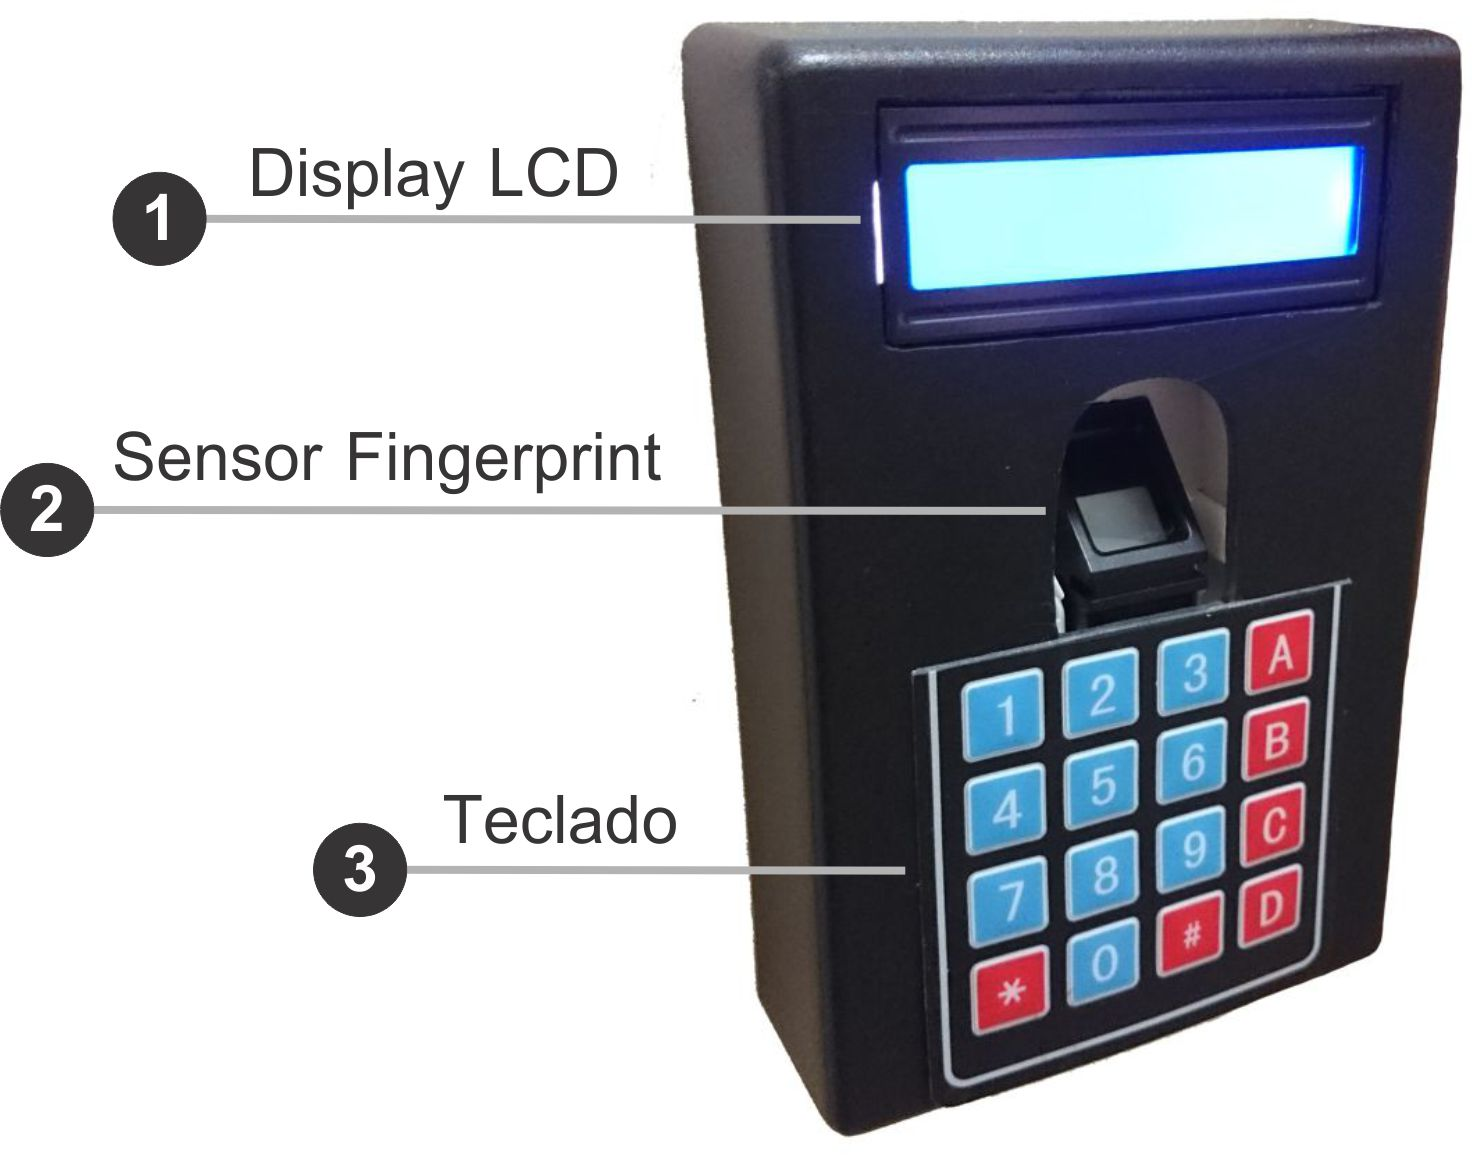
\includegraphics[scale=0.2]{figuras/cap4/setfinger_v2.jpg}\\
  Fonte: Elaborada pelo autor.
  \label{setfinger_v2}
  \end{center}
  \end{figure}

\begin{figure}[!ht]
  \begin{center}
  \caption{Segunda versão de \textit{hardware} (SetFinger 2.0) - módulo de \textit{hardware} interno composto por um Arduino Mega 2560, um ethernet shield W5100 e um Setshield 2.0. Esse módulo deve ser instalado fora do alcance dos usuários, preferencialmente no interior da sala a ser controlada.}
  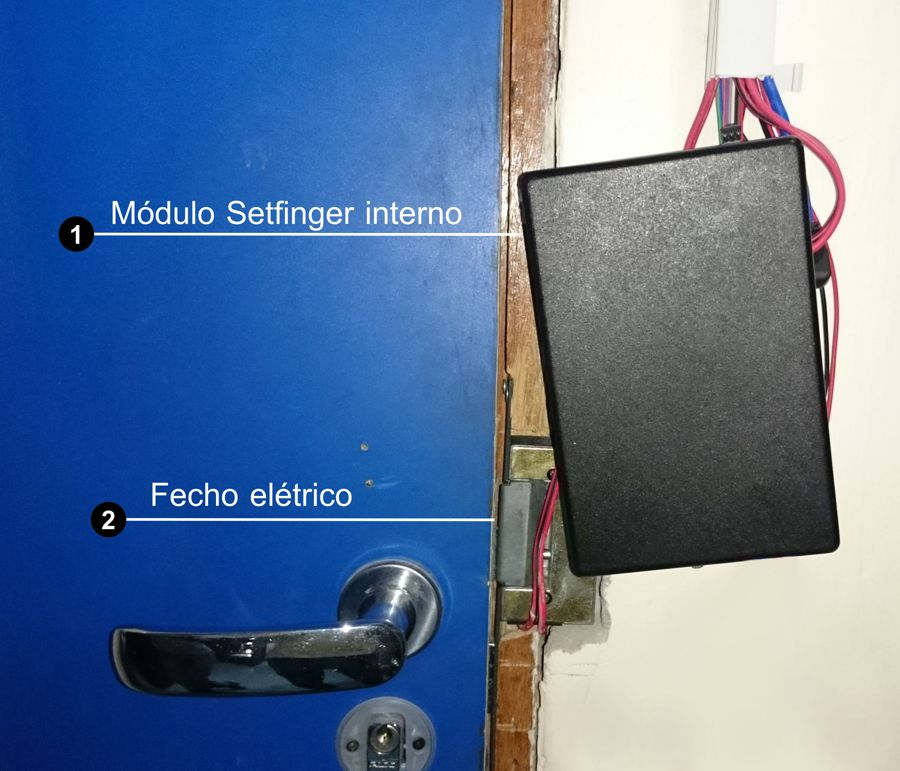
\includegraphics[scale=0.5]{figuras/cap4/setfinger_v2_p2.jpg}\\
  Fonte: Elaborada pelo autor.
  \label{setfinger_v2_p2}
  \end{center}
  \end{figure}
  

\begin{figure}[!ht]
  \begin{center}
  \caption{Placa Setshield 2.0.}
  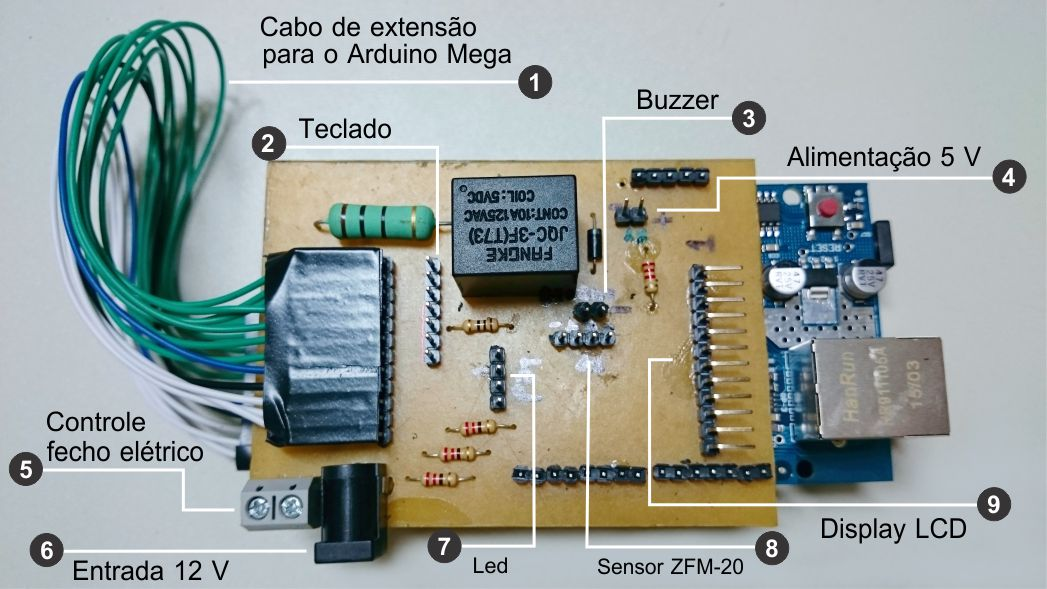
\includegraphics[scale=0.55]{figuras/cap4/setshield_v2.jpg}\\
  Fonte: Elaborada pelo autor.
  \label{setshield_v2}
  \end{center}
  \end{figure}


\chapter{Esquemático da placa Setshield \label{schematic_setshield}}

Esquemático da placa Setshield projetada no \textit{softwate} CadSoft Eagle 7.5.0.
  \begin{center}
  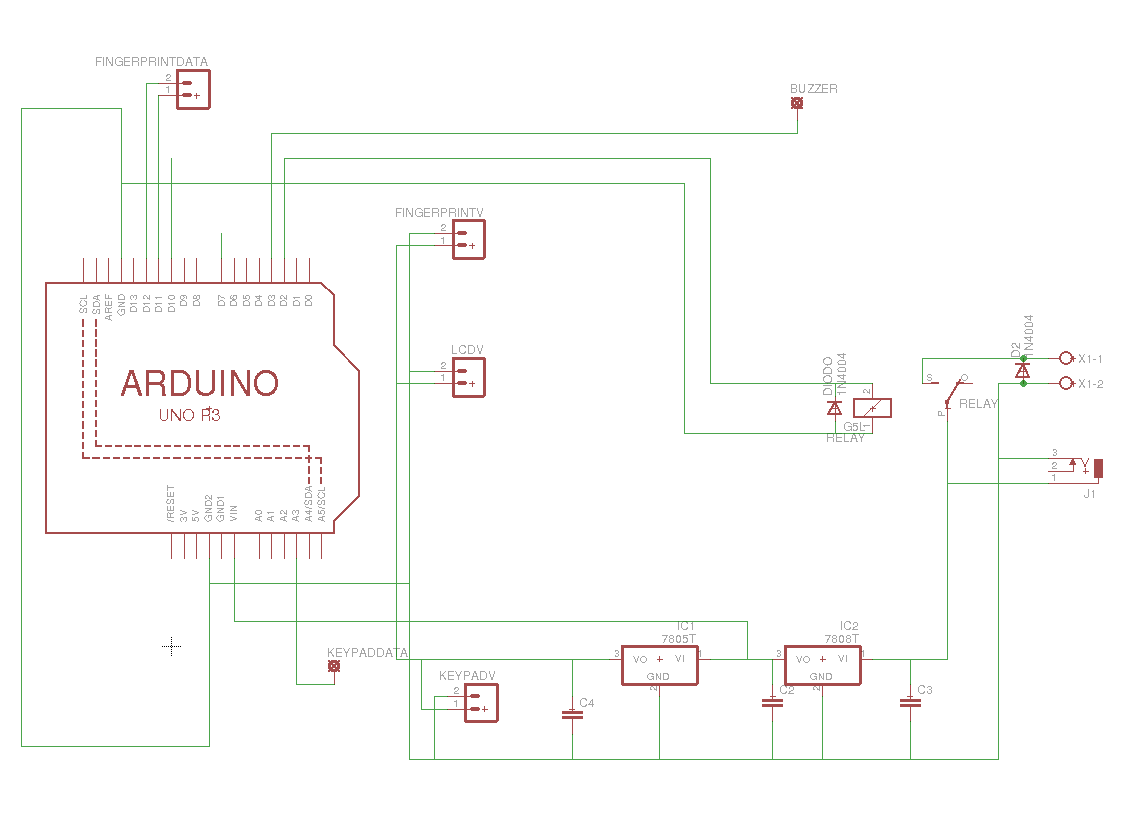
\includegraphics[scale=0.55]{figuras/anexos_e_apendices/schematic_setshield.png}\\
  Fonte: Elaborada pelo autor.
  \end{center}


\chapter{Design da placa Setshield \label{board_setshield}}

Design da placa Setshield projetada no \textit{softwate} CadSoft Eagle 7.5.0.

  \begin{center}
  \includegraphics[scale=0.55]{figuras/anexos_e_apendices/board_setshield.png}\\
  Fonte: Elaborada pelo autor.
  \end{center}
  
\newpage
%%%%%%%%%%%%%%%%%%%%%%%%%%%%%%%%%%
%   Referencias bibliograficas   %
%%%%%%%%%%%%%%%%%%%%%%%%%%%%%%%%%%

\addcontentsline{toc}{chapter}{Referências Bibliográficas}
%\renewcommand\bibname{Referências Bibliográficas}
% \bibliographystyle{IEEEtran}
% \bibliography{bibli}
\bibliographystyle{IEEEtran}
\bibliography{IEEEabrv,abrv,bibli}
% \clearpage






\end{document}

